% ----------------------------------------------------------------------
%                   Latex File for Joseph Roche's PhD (2012)
% ----------------------------------------------------------------------

%Latext thesis template from Harish Bhanderi's PhD/MPhil template, then Uni Cambridge
% http://www-h.eng.cam.ac.uk/help/tpl/textprocessing/ThesisStyle/

%: Style file for Latex
% Most style definitions are in the external file PhDthesisPSnPDF.
% In this template package, it can be found in ./Latex/Classes/
\documentclass[a4paper,oneside,12pt,usenatbib]{Latex/Classes/PhDthesisPSnPDF}
\setcitestyle{numbers}

%Change "oneside" to "twoside" for final submission-grade thesis after viva/corrections


\usepackage{amsbsy}
\usepackage{amsmath}
\usepackage{caption}
\usepackage{comment}
\usepackage{epstopdf}
\usepackage{fancyhdr}
\usepackage{hyperref}
\usepackage{lineno}
\usepackage{lscape}
\usepackage{multirow}
\usepackage{natbib}
\usepackage{paralist}
\usepackage{quotchap}
\usepackage{rotating}
\usepackage{setspace}
\usepackage{sidecap}
\usepackage{siunitx}
\usepackage{subcaption}
\usepackage{textcomp}
%\usepackage{titlesec}
\usepackage{url}
\usepackage{wrapfig}
\usepackage{wtmmPkg}
\usepackage{xspace}

\usepackage[font={footnotesize}]{caption}
\usepackage[capitalise]{cleveref}
\usepackage[left=2.5cm, right=2.5cm, top=3.3cm, bottom=2.0cm, footskip=1cm]{geometry}
\usepackage[font={footnotesize}]{subcaption}

\Crefname{figure}{Fig.}{Figs.}% {<type>}{<singular>}{<plural>}

\renewcommand{\bibpreamble}{\begin{multicols}{2}}
\renewcommand{\bibpostamble}{\end{multicols}}


%\usepackage{geometry}

%%% Added by DOF Jan 2018
% This gets rid of ugly hyperlink boxes for pdf versions
% Replaces boxes with changed text colour.
% Looks way better
\usepackage{xcolor}
%% for pdf use this:
  \hypersetup{
      colorlinks,
      linkcolor={red},
      citecolor={blue!80!black},
      urlcolor={blue!80!black}
  }
%% for printing use this:
%\hypersetup{
%    colorlinks,
%    linkcolor=.,
%    citecolor=.,
%    urlcolor=.
%      }

\creflabelformat{equation}{#2\textup{#1}#3}

%\usepackage{showframe}

%%%
% Added by DOF Jan 2018 to make nicer chapter numbers
% comment out next lines to revert to default
% (Don't forget to uncomment titlesec package above!!!!)
%%%
\usepackage{color}
\definecolor{RoyalRed}{RGB}{157,16, 45}
%\renewcommand{\sfdefault}{mdugm} %Garamond
\usepackage[ ]{titlesec}  %
\titleformat{\chapter}[display]
  { \normalsize \huge  \color{RoyalRed}}
  {\flushright \normalsize \color{RoyalRed} \MakeUppercase {} \vspace{-45mm} \hspace{1 ex} { \fontsize{55}{55}\selectfont \color{RoyalRed} \sffamily  \thechapter }} {10 pt}{\raggedleft \Huge}
\titlespacing{\chapter}{0pt}{50pt}{5mm}%


%Added by SM 13 Sep 2011 to get backref to read ''Cited on page''
%   \usepackage{Latex/StyleFiles/backrefx}
%       \renewcommand{\backrefpagesname}{Cited on page~}
%       \renewcommand{\backrefpagesnames}{Cited on pages~}

\newcommand{\BibTeX}{\textsc{Bib}\TeX}
\newcommand{\etal}{{\it et al.}}

% Definitions for equations
\newcommand{\arcsec}{^{\prime\prime}}
%\def\ion#1#2{#1$\;${\small\rm\@Roman{#2}}\relax}
\DeclareRobustCommand{\ion}[2]{%
\relax\ifmmode
\ifx\testbx\f@series
{\mathbf{#1\,\mathsc{#2}}}\else
{\mathrm{#1\,\mathsc{#2}}}\fi
\else\textup{#1\,{\mdseries\textsc{#2}}}%
\fi}

\newcommand{\subion}{ {_{ion}} }
\newcommand{\sube}{ {_{e}} }
\newcommand{\subj}{ {_{j}} }
\newcommand{\subi}{ {_{i}} }
\newcommand{\ji}{ {_{j,i}} }
\newcommand{\rt}{ {$R(T)$} }
\newcommand{\rlam}{ {$R(\lambda)$} }
\newcommand{\rsun}{R$_{\odot}$}
\newcommand{\rmd}{ {\ \mathrm d} }
\renewcommand{\vec}[1]{ {\mathbf #1} }
\newcommand{\uvec}[1]{ \hat{\mathbf #1} }
\newcommand{\pder}[2]{ \f{\partial #1}{\partial #2} }
\newcommand{\grad}{ {\bf \nabla } }
\newcommand{\curl}{ {\bf \nabla} \times}
\newcommand{\vol}{ {\mathcal V} }
\newcommand{\bndry}{ {\mathcal S} }
\newcommand{\dv}{~{\mathrm d}^3 x}
\newcommand{\da}{~{\mathrm d}^2 x}
\newcommand{\dl}{~{\mathrm d} l}
\newcommand{\dt}{~{\mathrm d}t}
\newcommand{\intv}{\int_{\vol}^{}}
\newcommand{\inta}{\int_{\bndry}^{}}
\newcommand{\avec}{ \vec A}
\newcommand{\ap}{ \vec A_p}
\newcommand{\bb}{ \vec B}
\newcommand{\jj}{ \vec j}
\newcommand{\rr}{ \vec r}
\newcommand{\xx}{ \vec x}

% Definitions for the journal names
\newcommand{\adv}{    {\it Advances in Space Research}}
\newcommand{\annG}{   {\it Annales Geophysicae}}
\newcommand{\aap}{    {\it Astronomy \& Astrophysics}}
\newcommand{\aaps}{   {\it Astronomy \& Astrophysics Supplemental}}
\newcommand{\aapr}{   {\it Astronomy \& Astrophysics Review}}
\newcommand{\ag}{     {\it Ann. Geophys.}}
\newcommand{\aj}{     {\it Astronomical Journal}}
\newcommand{\apj}{    {\it Astrophysical Journal}}
\newcommand{\apjs}{    {\it Astrophysical Journal Supplemental Series}}
\newcommand{\apjl}{   {\it Astrophysical Journal Letters}}
\newcommand{\apss}{   {\it Astrophysics \& Space Science}}
\newcommand{\cjaa}{   {\it Chinese Journal Astronomy \& Astrophysics}}
\newcommand{\gafd}{   {\it Geophysical and Astrophysical Fluid Dynamics}}
\newcommand{\grl}{    {\it Geophysical Research Letters}}
\newcommand{\ijga}{   {\it International Journal of Geomagnetism and Aeronomy}}
\newcommand{\jastp}{  {\it Journal of Atmospheric and Solar-Terrestrial Physics}}
\newcommand{\jgr}{    {\it Journal of Geophysical Research}}
\newcommand{\mnras}{  {\it Monthly Notices of the Royal Astronomical Society}}
\newcommand{\nat}{    {\it Nature}}
\newcommand{\pasp}{   {\it Publications of the Astronomical Society of the Pacific}}
\newcommand{\pasj}{   {\it Publications of the Astronomical Society of Japan}}
\newcommand{\pra}{    {\it Physical Review A}}
\newcommand{\pre}{    {\it Physical Review E}}
\newcommand{\solphys}{{\it Solar Physics}}
\newcommand{\sovast}{ {\it Soviet Astronomy}}
\newcommand{\ssr}{    {\it Space Science Reviews}}
\newcommand{\araa}{  {\it Annual Review of Astronomy \& Astrophysics}}
\newcommand{\memsai}{ {\it Memorie della Societa Astronomia Italiana}}
\newcommand{\planss}{ {\it Planetary and Space Science} }
\newcommand{\actaa}{ {\it Acta Astronomica} }
\newcommand{\zap}{ {\it Zeitschrift für Astrophysik} }
%: Macro file for Latex
% Macros help you summarise frequently repeated Latex commands.
% Here, they are placed in an external file /Latex/Macros/MacroFile1.tex
% An macro that you may use frequently is the figuremacro (see introduction.tex)
% This file contains macros that can be called up from connected TeX files
% It helps to summarise repeated code, e.g. figure insertion (see below).

% insert a centered figure with caption and description
% parameters 1:filename, 2:title, 3:description and label
\newcommand{\figuremacro}[3]{
	\begin{figure}[htbp]
		\centering
		\includegraphics[width=1\textwidth]{#1}
		\caption[#2]{\textbf{#2} - #3}
		\label{#1}
	\end{figure}
}

% insert a centered figure with caption and description AND WIDTH
% parameters 1:filename, 2:title, 3:description and label, 4: textwidth
% textwidth 1 means as text, 0.5 means half the width of the text
\newcommand{\figuremacroW}[4]{
	\begin{figure}[htbp]
		\centering
		\includegraphics[width=#4\textwidth]{#1}
		\caption[#2]{\textbf{#2} - #3}
		\label{#1}
	\end{figure}
}

% inserts a figure with wrapped around text; only suitable for NARROW figs
% o is for outside on a double paged document; others: l, r, i(inside)
% text and figure will each be half of the document width
% note: long captions often crash with adjacent content; take care
% in general: above 2 macro produce more reliable layout
\newcommand{\figuremacroN}[3]{
	\begin{wrapfigure}{o}{0.5\textwidth}
		\centering
		\includegraphics[width=0.48\textwidth]{#1}
		\caption[#2]{{\small\textbf{#2} - #3}}
		\label{#1}
	\end{wrapfigure}
}

% predefined commands by Harish
\newcommand{\PdfPsText}[2]{
  \ifpdf
     #1
  \else
     #2
  \fi
}

\newcommand{\IncludeGraphicsH}[3]{
  \PdfPsText{\includegraphics[height=#2]{#1}}{\includegraphics[bb = #3, height=#2]{#1}}
}

\newcommand{\IncludeGraphicsW}[3]{
  \PdfPsText{\includegraphics[width=#2]{#1}}{\includegraphics[bb = #3, width=#2]{#1}}
}

\newcommand{\InsertFig}[3]{
  \begin{figure}[!htbp]
    \begin{center}
      \leavevmode
      #1
      \caption{#2}
      \label{#3}
    \end{center}
  \end{figure}
}


%%% Local Variables: 
%%% mode: latex
%%% TeX-master: "~/Documents/LaTeX/CUEDThesisPSnPDF/thesis"
%%% End: 


%Change this if compiling at home/office
%\graphicspath{{/Users/josephroche/Work/log_of_learning/images/}}
\graphicspath{{Images/}}


%: --------------------------------------------------------------
%:                  FRONT MATTER: dedications, abstract,..
% --------------------------------------------------------------

\usepackage{setspace}
\singlespacing
\graphicspath{{./}{Images/}}
\begin{document}

\setcitestyle{authoryear}

\renewcommand\baselinestretch{1.2}
\baselineskip=18pt plus1pt

%: ----------------------- COVER PAGE ------------------------

\newcommand{\titlefont}{\bfseries \fontsize{22}{26.42pt}\selectfont}
\newcommand{\largetitlefont}{\bfseries \fontsize{29.88}{35.88pt}\selectfont}
\newcommand{\othertitlefont}{\fontsize{14.4}{17.28}\selectfont}
\newcommand{\authorfont}{\bfseries \fontsize{14.4}{17.28}\selectfont}
\newcommand{\informationfont}{\fontsize{10}{12}\selectfont}
\newcommand{\dedicationfont}{\slshape \fontsize{14.4}{17.28}\selectfont}

\newcommand{\thisyear}{\number\year}
\def\thismonth{\ifcase\month\or January\or February\or March\or
  April\or May\or June\or July\or August\or September\or October\or November\or December\fi}
\newcommand{\todaysdate}{\thismonth\space \thisyear}

\renewcommand{\baselinestretch}{1}
\newpage \thispagestyle{empty}
\vspace*{1.5cm}
\begin{flushright}


%TITLE

\Huge{\textbf{Probing the Solar Corona at High Temporal and Spatial Resolution with the LOw Frequency ARray (LOFAR)}}

\end{flushright}

\vspace*{3cm}
\begin{flushright}
A dissertation submitted to the University of Dublin \\
for the degree of Doctor of Philosophy
\end{flushright}

\vspace*{\fill}
\begin{flushright}
{\authorfont {Pearse Murphy, B.A.\ (Mod.)} \\[1mm]
{\textnormal{\textit{School of Physics, Trinity College Dublin}}\\}

\vspace*{\fill}
\begin{flushright}
\textnormal{
\textit{Supervisor:} \\
Prof. Peter T. Gallagher}\\[0.5mm]
\textnormal{
\textit{Co-Supervisor:} \\
Dr. Eoin P. Carley}\\[0.5mm]
\end{flushright}
{December 2021}\\[5mm]
\rule{0.9\textwidth}{0.5mm}\\[4mm]
%
\begin{figure}[ht!]
\hspace{102mm}
\raggedleft

\includegraphics[height=20mm]{tcd_logo.png}
\end{figure}

}%
\end{flushright}

%: -----------------------tie in front matter------------------------

\frontmatter
\begin{declaration}      

%I have read and I understand the plagiarism provisions in the General Regulations of the University Calendar for the current year, found at: \url{https://www.tcd.ie/calendar}
%
%I have also completed the Online Tutorial on avoiding plagiarism ‘Ready, Steady, Write’, located at \url{http://tcd-ie.libguides.com/plagiarism/ready-steady-write}  
%
%\vspace{10mm}
%
%%I declare that this report is my own work, is not copied from any other person's work (published or unpublished), and has not previously submitted for assessment either at Trinity College Dublin or elsewhere.
%I declare that this thesis has not been submitted as an exercise for a degree at this or any other university and it is entirely my own work. 
I agree to deposit this thesis in the University's open access institutional repository or allow the Library to do so on my behalf, subject to Irish Copyright Legislation and Trinity College Library conditions of use and acknowledgement.

I consent to the examiner retaining a copy of the thesis beyond the examining period, should they so wish (EU GDPR May 2018). 

\vspace{30mm}

\textbf{Name:} Pearse Murphy

\vspace{15mm}

\textbf{Signature:}  ........................................		\textbf{Date:}  10/12/2021

\end{declaration}

\newpage
\thispagestyle{empty}
\mbox{}

%!TEX root = ../main.tex
%Adding the above line, with the name of your base .tex file (in this case "thesis.tex") will allow you to compile the whole thesis even when working inside one of the chapter tex files
\newgeometry{left=2.5cm, right=2.5cm, top=2.0cm, bottom=2.0cm, footskip=1cm}
\begin{abstracts} 

The solar corona is the outermost layer of the Sun's atmosphere. Advancements in radio astronomy over the last 50 years have revealed a number of radio phenomena which occur in the corona each with different temporal and spectral characteristics. Current generation interferometers such as the LOw Frequency ARray (LOFAR) give an unprecedented insight into the fine structure of these radio bursts. Of particular interest are what are known as Type III radio bursts. These are indicative of electrons being accelerated along open magnetic field lines in the solar corona. Particularly bright radio bursts can have devastating effects on terrestrial communication including GPS positioning and satellite communication. Given that much of modern society relies on satellite communication, being better able to understand and perhaps predict radio bursts is essential. High temporal resolution data allow the study of rapid temporal variability in radio spectra which are indicative of small-scale turbulence in the solar corona. It is thought that the density inhomogeneities produced by this small-scale turbulence causes scattering of radio waves as they propagate out from the corona and thus pose a fundamental limit on the source size of observed radio bursts. Analysis of a radio burst at the plasma frequency, such as a Type III burst, with highly spatially resolved interferometric data is the most direct way of testing this hypothesis.% and is one of the fundamental pieces of this PhD. Following this, exploratory work with 5 ns temporal resolution data from the Irish LOFAR station (I-LOFAR) to delve further into the small-scale variations with time in the solar corona will be undertaken.

The nature of this PhD is twofold, firstly to observe low frequency radio emission from the Sun at spatial resolution of the order of 15 arcseconds. This will determine whether or not scattering of radio waves in the corona imposes a fundamental limit on spatial resolution and give insight into the processes that might cause this limit. The second aspect of this PhD is to observe the Sun at radio wavelengths at the highest temporal resolution ever. In order to do this, the TBB Acquisition Cluster (TACl) located in the I-LOFAR control room must be further developed to record and store TBB data without corruption. Observing the Sun at nanosecond temporal resolution has yet to be attempted and as such the potential to discover new radio phenomena and temporal variability in existing phenomena is great. It is, of course, possible that such events do not occur or are difficult to detect and as such the focus for this PhD will lie mainly on interferometric observations of the Sun.

%The goal for this project is to study known radio phenomena at nanosecond resolution in order to discover new temporal variability, if this exists, and new sub-microsecond radio bursts if they exist. In order to do this a computer cluster dedicated to the recording and storage of such data, which is real, must be further developed

This report is an overview of my PhD thus far and is as follows. Chapter \ref{chap:intro} describes the Sun and the corona. It introduces the role radio bursts have to play in determining source sizes in the corona and outlines the theory behind plasma emission, radio interferometry and beam-forming. Chapter \ref{chap:inst} gives a technical description of LOFAR, its hardware and the digital signal processing pipeline of an international LOFAR station. Observations using high temporal resolution data from I-LOFAR are explained in chapter \ref{chap:obs} along with interferometric images from the core and remote LOFAR stations. The results of analysis of this data is also given in chapter \ref{chap:obs} before the report is concluded in \ref{chap:conc}. Future work for this PhD is outlined in chapter \ref{chap:future}.
\end{abstracts}


\restoregeometry



% ---------------------------------------------------------------------- 
% ---------------------------------------------------------------------- 



%!TEX root = ../thesis.tex
%Adding the above line, with the name of your base .tex file (in this case "thesis.tex") will allow you to compile the whole thesis even when working inside one of the chapter tex files


\begin{declaration}      

I have read and I understand the plagiarism provisions in the General Regulations of the University Calendar for the current year, found at: \url{https://www.tcd.ie/calendar}

I have also completed the Online Tutorial on avoiding plagiarism ‘Ready, Steady, Write’, located at \url{http://tcd-ie.libguides.com/plagiarism/ready-steady-write}  

\vspace{10mm}

I declare that this report is my own work, is not copied from any other person's work (published or unpublished), and has not previously submitted for assessment either at Trinity College Dublin or elsewhere.

\vspace{30mm}

\textbf{Name:} Pearse Murphy

\vspace{15mm}

\textbf{Signature:}  ........................................		\textbf{Date:}  ..........................

\end{declaration}

% ----------------------------------------------------------------------





%!TEX root = ../thesis.tex
%Adding the above line, with the name of your base .tex file (in this case "thesis.tex") will allow you to compile the whole thesis even when working inside one of the chapter tex files
\chapter{List of Publications}
\label{chapter:publications}
%
\begin{singlespace}
\vspace{-5mm}

%
\section*{Oral Presentations}
\begin{enumerate}
\item \textit{Finding Fast Solar Radio Transients in I-LOFAR Transient Buffer Board Data},\\ Irish National Astronomy Meeting (INAM), 2018
\item \textit{Finding Fast Solar Radio Transients in I-LOFAR Transient Buffer Board Data},\\ Community of European Solar Radio Astronomers (CESRA) Summer School, 2018
\end{enumerate}

%
\section*{Poster Presentations}
\begin{enumerate}
\item \textit{The Irish LOw Frequency ARray (I-LOFAR)}, \\ International Workshop on Solar, Heliospheric and Magnetospheric Radioastronomy, 2017
\\ DOI: \url{https://doi.org/10.6084/m9.figshare.5572660.v1}
\item \textit{Nanosecond Sampling of the Radio Sky with I-LOFAR's Transient Buffer Boards (TBB)}, \\ 17th RHESSI (Reuven Ramaty High Energy Solar Spectroscopic Imager) Workshop, 2018
\\ DOI: \url{https://doi.org/10.6084/m9.figshare.6669173.v1}
\end{enumerate}


%
\section*{Workshops \& Conferences Attended}
\begin{enumerate}
\item INAM, Maynooth University, 2017
\item International Workshop on Solar, Heliospheric and Magnetospheric Radioastronomy, Observatoire de Paris, 2017
\item I-LOFAR User's Data Workshop, University College Dublin, 2018
\item 17th RHESSI Workshop, Trinity College Dublin, 2018
\item Astro Hack Week, Lorentz Cetnre, Leiden University, 2018
\item INAM, Birr Theatre, Birr, Co. Offaly, 2018
\item CESRA Summer School, Observatoire Royal de Belgique, 2018 
\item LOFAR Data Processing School, Netherlands Institute for Radio Astronomy (ASTRON), 2018
\end{enumerate}

\section*{Publications}
\begin{enumerate}
\item David M. Long, \textbf{Pearse C. Murphy}, Georgina Graham, Eoin P. Carley, David P\'{e}rez-Su\'{a}rez.
\\ ``A Statistical Analysis of the Solar Phenomena Associated with Global EUV Waves",
\\ \textit{Solar Physics}, Volume 292 , Issue 185, (2017).
%Long, D.M., \textbf{Murphy, P. C.}, Graham, G. et al. Sol Phys (2017) 292: 185. \doihttps{https://doi.org/10.1007/s11207-017-1206-0}
\end{enumerate}




\end{singlespace}





\chapter{List of Publications}
\label{chapter:publications}
%
\begin{singlespace}
\vspace{-5mm}

%
%\section*{Oral Presentations}
%\begin{enumerate}
%STELLAR Space Weather Workshop
%Virtual
%12th - 15th July 2021
%
%\item \textit{LOFAR Single Station Radio Data Analysis Tutorial}
%I-LOFAR Science and Techniques Workshop
%I-LOFAR Education Centre, Birr Castle, Co. Offaly, Ireland
%2nd - 4th March 2020
%
%Scattering of Radio Waves in the Solar Corona
%I-LOFAR Science and Techniques Workshop
%I-LOFAR Education Centre, Birr Castle, Co. Offaly, Ireland
%2nd - 4th March 2020
%
%Single Station Data Analysis Tutorial
%Young European Radio Astronomers Conference
%Dublin Institute for Advanced Studies/Trinity College Dublin, Ireland
%26th - 29th August 2019
%
%Interferometric Imaging of Type III Bursts in the Solar Corona
%Community of European Solar Radio Astronomers Workshop
%Leibniz-Institut für Astrophysik Potsdam, Germany
%8th - 12th July 2019
%
%Interferometric Imaging of Type III Bursts in the Solar Corona
%\item \textit{Finding Fast Solar Radio Transients in I-LOFAR Transient Buffer Board Data},\\ Irish National Astronomy Meeting (INAM), 2018
%\item \textit{Finding Fast Solar Radio Transients in I-LOFAR Transient Buffer Board Data},\\ Community of European Solar Radio Astronomers (CESRA) Summer School, 2018
%\end{enumerate}
%
%%
%\section*{Poster Presentations}
%\begin{enumerate}
%\item \textit{The Irish LOw Frequency ARray (I-LOFAR)}, \\ International Workshop on Solar, Heliospheric and Magnetospheric Radioastronomy, 2017
%\\ DOI: \url{https://doi.org/10.6084/m9.figshare.5572660.v1}
%\item \textit{Nanosecond Sampling of the Radio Sky with I-LOFAR's Transient Buffer Boards (TBB)}, \\ 17th RHESSI (Reuven Ramaty High Energy Solar Spectroscopic Imager) Workshop, 2018
%\\ DOI: \url{https://doi.org/10.6084/m9.figshare.6669173.v1}
%\end{enumerate}
%
%
%%
%\section*{Workshops \& Conferences Attended}
%\begin{enumerate}
%\item INAM, Maynooth University, 2017
%\item International Workshop on Solar, Heliospheric and Magnetospheric Radioastronomy, Observatoire de Paris, 2017
%\item I-LOFAR User's Data Workshop, University College Dublin, 2018
%\item 17th RHESSI Workshop, Trinity College Dublin, 2018
%\item Astro Hack Week, Lorentz Cetnre, Leiden University, 2018
%\item INAM, Birr Theatre, Birr, Co. Offaly, 2018
%\item CESRA Summer School, Observatoire Royal de Belgique, 2018 
%\item LOFAR Data Processing School, Netherlands Institute for Radio Astronomy (ASTRON), 2018
%\end{enumerate}

\section*{Publications}
\begin{enumerate}
\item Corentin K. Louis, Caitriona M. Jackman, Jean-Mathias Griessmeier, Olaf Wucknitz, David. J. McKenna, \textbf{Pearse C. Murphy}, Peter T. Gallagher, Eoin Carley, Dúalta Ó Fionnagáin, Aaron Golden, Joe McCauley, Paul Callanan, Matt Redman, Christian Vocks.
\\``Observing Jupiter's radio emissions using multiple LOFAR stations: a first case study of the Io-decametric emission using the Irish IE613, French FR606 and German DE604 stations"
\\ \textit{Royal Astronomical Society Techniques and Instruments journal} (2021 submitted)
\item \textbf{P. C. Murphy}, P. Callanan, J. McCauley, D. J. McKenna, D. Ó Fionnagáin, C. K. Louis, M. P. Redman, L. A. Cañizares, E. P. Carley, S. A. Maloney, B. Coghlan, M. Daly, J. Scully, J. Dooley, V. Gajjar, C. Giese, A. Brennan, E. F. Keane, C. A. Maguire, J. Quinn, S. Mooney, A. M. Ryan, J. Walsh, C. M. Jackman, A. Golden, T. P. Ray, J. G. Doyle, J. Rigney, M. Burton, P. T. Gallagher.
\\``First Results from the REAL-time Transient Acquisition backend (REALTA) at the Irish LOFAR station",
\\ \textit{Astronomy and Astrophysics} Volume 655, A16 (2021)
\item A. M. Ryan, P. T. Gallagher, E. P. Carley, M. A. Brentjens,\textbf{ P. C. Murphy}, C. Vocks, D. E. Morosan, H. Reid, J. Magdalenic, F. Breitling, P. Zucca, R. Fallows, G. Mann, A. Kerdraon, R. Halfwerk.
\\``LOFAR imaging of the solar corona during the 2015 March 20 solar eclipse",
\\ \textit{Astronomy and Astrophysics}, Volume 648, A43 (2021)
\item \textbf{Pearse C. Murphy}, Eoin P. Carely, Aoife Maria Ryan, Pietro Zucca, Peter T. Gallagher.
\\ ``LOFAR Observations of Radio Burst Source Sizes and Scattering in the Solar Corona",
\\ \textit{Astronomy and Astrophysics}, Volume 645, A11 (2021)
\item Vishal Gajjar, Andrew Siemion, Steve Croft, Bryan Brzycki, Marta Burgay, Tobia Carozzi, Raimondo Concu, Daniel Czech, David DeBoer, Julia DeMarines, Jamie Drew, J. Emilio Enriquez, James Fawcett, Peter Gallagher, Michael Gerret, Nectaria Gizani, Greg Hellbourg, Jamie Holder, Howard Isaacson, Sanjay Kudale, Brian Lacki, Matthew Lebofsky, Di Li, David H. E. MacMahon, Joe McCauley, Andrea Melis, Emilio Molinari, \textbf{Pearse Murphy}, Delphine Perrodin, Maura Pilia, Danny C. Price, Claire Webb, Dan Werthimer, David Williams, Pete Worden, Philippe Zarka, and Yunfan Gerry Zhang.
\\``The Breakthrough Listen Search for Extraterrestrial Intelligence ",
\\ \textit{Astro2020: Decadal Survey on Astronomy and Astrophysics, APC white papers, no. 223; Bulletin of the American Astronomical Society}, Vol. 51, Issue 7, id. 223 (2019)
\item David M. Long, \textbf{Pearse C. Murphy}, Georgina Graham, Eoin P. Carley, David P\'{e}rez-Su\'{a}rez.
\\ ``A Statistical Analysis of the Solar Phenomena Associated with Global EUV Waves",
\\ \textit{Solar Physics}, Volume 292 , Issue 185, (2017).
%Long, D.M., \textbf{Murphy, P. C.}, Graham, G. et al. Sol Phys (2017) 292: 185. \doihttps{https://doi.org/10.1007/s11207-017-1206-0}
\end{enumerate}




\end{singlespace}





%: ----------------------- contents ------------------------

\setcounter{secnumdepth}{3} % organisational level that receives a numbers
\setcounter{tocdepth}{3}    % print table of contents for level 3
\tableofcontents            % print the table of contents
% levels are: 0 - chapter, 1 - section, 2 - subsection, 3 - subsection


%: ----------------------- list of figures/tables ------------------------

\listoffigures	% print list of figures
%\listoftables  % print list of tables


%: --------------------------------------------------------------
%:                  MAIN DOCUMENT SECTION
% --------------------------------------------------------------


\mainmatter

\pagestyle{fancy}
%\fancyhf{}
%\rhead{\leftmark}
%\lhead{\leftmark}
%!TEX root = ../main.tex
%Adding the above line, with the name of your base .tex file (in this case "thesis.tex") will allow you to compile the whole thesis even when working inside one of the chapter tex files
%: ----------------------- introduction file header -----------------------
\doublespacing
\chapter{Introduction}
\label{chap:intro}
Ancient passage tombs in Ireland show evidence that thousands of years ago, humans had an understanding of the movement of the Sun in the sky at different times of the year. These tombs are constructed such that only on the day of a solar solstice or equinox, is the passageway illuminated in full. Today the Sun is still a source of curiosity and has more than once shown that us humans are not the centre of the universe. The light and heat from the Sun are the essential source of energy for life on our planet however, our proximity to this star also comes with a risk. Explosive and energetic events such as coronal mass ejections and solar flares occur with varying frequency and intensity over the course of an eleven year cycle. Their effects on Earth were made known in a spectacular fashion in 1859 with the so called \textit{Carrington Event}. This was a solar eruptive event, the magnitude of which has not been seen in the subsequent 162 years. It induced currents into telegraph wires causing them to operate even though they had been removed from a power source. It also caused aurora to be seen as close to the equator as Cuba and bright enough at higher latitudes that a newspaper could be read at night time under their light. 

The Sun emits across the electromagnetic spectrum however, the focus of this thesis is low frequency radio waves. Similar mechanisms that drive large energy releases like the Carrington Event also generate radio wave emission in the form of ``solar radio bursts". These solar radio bursts can be used as a remote diagnostic of the Sun's atmosphere and determine the microphysics of the plasma that in the outer layers of the solar atmosphere.
This chapter highlights some fundamental concepts of solar physics, different types of radio emission from the Sun and the implications of their study.

\section{The Sun}
The Sun is our nearest star and the centre of our solar system however, apart from these distinctions it is an average star. It is a G2 type star located on the main sequence of the Hertzsprung Russell diagram. It has a luminosity of $(3.83 \pm 0.04) \times 10^{26}$ W and a radius R$_\odot = (6.959 \pm 0.007) \times 10^8$ m \citep{Foukal2004}. The Sun's mass of $(1.9889 \pm 0.0003) \times 10^{30}$ kg comprises $>$ 99\% of the solar system's total mass \citep{Foukal2004}. At the time of writing, the Sun is $\sim$ 5 billion years old. Formed from a cooling cloud of gas and dust 4.6 billion years ago, the Sun now has a core with a temperature of 15 MK. This temperature is hot enough for nuclear fusion to occur and will continue to do so until the Sun's supply of Hydrogen runs out. The Sun will remain on the main sequence for a further $\sim 5$ billion years before expanding into a Red Giant. %At this point the core will contract until the density reaches a density such that further condensation is prevented by the electron exclusion principle.   %There are a number of nuclear fusion processes in the Sun's core, the most common of which is the proton-proton or `pp' chain whereby four protons collide and fuse to form a Helium nucleus. The most frequent pp chain is known as ppI, it occurs 86\% of the time \citep{Turck-Chieze2011} and is as follows,
% $$
% ^1_1\mbox{H} + ^1_1\mbox{H} \rightarrow ^2_1\mbox{H} + e^+ + \nu_e
% $$
% $$
% ^2_1\mbox{H} + ^1_1\mbox{H} \rightarrow ^3_2\mbox{He} +\gamma
% $$
% $$
% ^3_2\mbox{He} + ^3_2\mbox{He} \rightarrow ^4_2\mbox{He} +2^1_1\mbox{H}
% $$
% Here, $^1_1\mbox{H}$ is a proton or Hydrogen nucleus, $^2_1\mbox{H}$ is its isotope Deuterium, $^3_2\mbox{He}$ is the Helium isotope Triteum, $^4_2\mbox{He}$ is Helium, $e^+$ is a positron, $\nu_e$ is an electron neutrino and $\gamma$ is a gamma ray photon. A complete ppI chain releases $4.2 \times 10^{-12}$ J of energy in the form of electromagnetic radiation. The energy output of all pp chains account for 98.8\% of the total energy produced by the Sun \citep{Turck-Chieze2011}. 

% Photons generated in the ppI travel outwards from the core however, their small mean free path of 0.9cm means that this takes on the order of $10^5$ years to reach the solar surface \citep{Mitalas1992}. At 70\% of the Sun's radius (0.7 R$_{\odot}$), the temperature has cooled to 1 MK thereby allowing electrons to bind to atomic orbitals, drastically decreasing the scattering rate of photons. Energy transfer from here to the solar surface at 1 R$_{\odot}$ is now primarily done through convection. 
Due to our proximity to the Sun, we are able to observe a vast array of phenomena, many of which have direct terrestrial impacts. These phenomena take place in the solar atmosphere and shall be described briefly below. The study of these phenomena is a study of the plasma and magnetic field structure of the solar atmosphere and gives insights into energy generation and transport.
\subsection{The Photosphere}
The layer of the Sun at 1 R$_{\odot}$ is known as the photosphere and is what would be called the surface of the Sun. The temperature of the photosphere, alternatively the surface temperature of the Sun, is $\sim 6000$~K and has a number density of the order of $10^{17} \mbox{cm}^{-3}$, at which point the mean free path of visible photons becomes much greater than the distance between the Sun and the Earth and can be thought as coming directly from the solar surface.

The most distinct feature of the photosphere in white light are sunspots. Sunspots are seen as dark regions in the photosphere and are the manifestation of of solar activity. Sunspot magnetic fields are much stronger than the surrounding magnetic field of the photosphere and as such, inhibit heat transfer. This means that sunspots are cooler $\sim 4200$~K \citep{McLean1985} than the surrounding plasma.
%At this point, the mean free path of visible photons becomes much greater than the distance between the Sun and the Earth and can be thought as coming directly from the solar surface.
%This is the point at which the optical depth for visible light photons is 1 and their mean free path is much greater than the distance between scattering centres on the solar surface. 

Above the photosphere the temperature and density profile change dramatically, see Figure \ref{fig:corona_temp}, throughout the remaining layers of the Sun's atmosphere; the chromosphere, the transition region and the corona. 
\begin{figure}[ht]
    \centering
    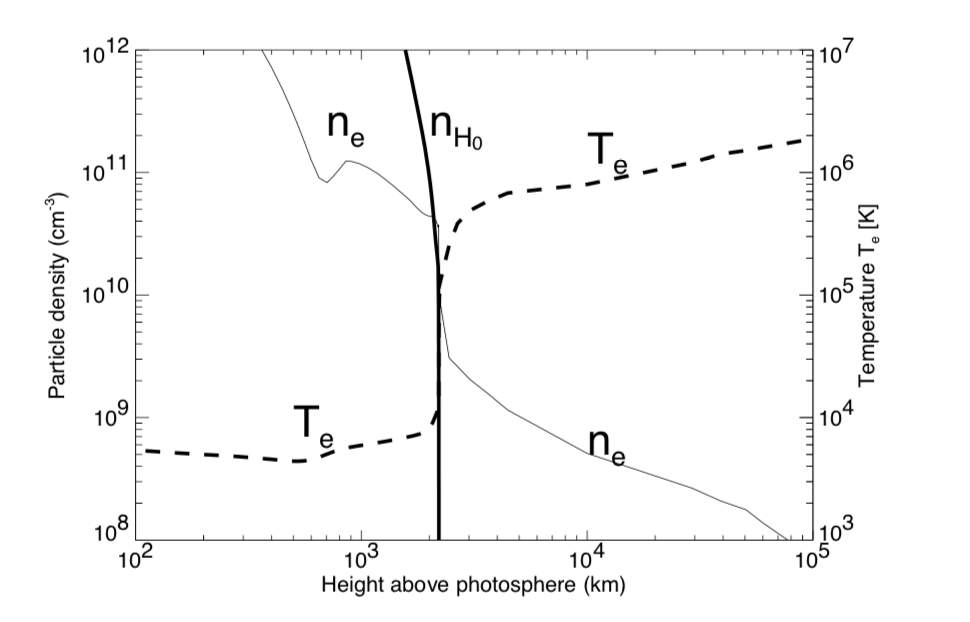
\includegraphics[width=\columnwidth]{Images/Corona_temp.png}
    \caption[Model of electron density and temperature with height in the solar atmosphere.]{Model of electron density and temperature with height in the solar atmosphere. The x axis shows height above the chromosphere in kilometres while the y axes show particle density in cm$^{-3}$ and temperature in Kelvin. The chromosphere begins $\sim 500$~km above the photosphere. The region around 2000 km showing a sharp rise in temperature and sharp fall in electron density is known as the transition region. Above this height plasma becomes fully ionised and is known as the corona. Image from \cite{Aschwanden2004}.}
    \label{fig:corona_temp}
\end{figure}
%Figure \ref{fig:Sun} shows the interior layers of the Sun and its atmosphere.
%\begin{figure}[t]
%    \centering
%    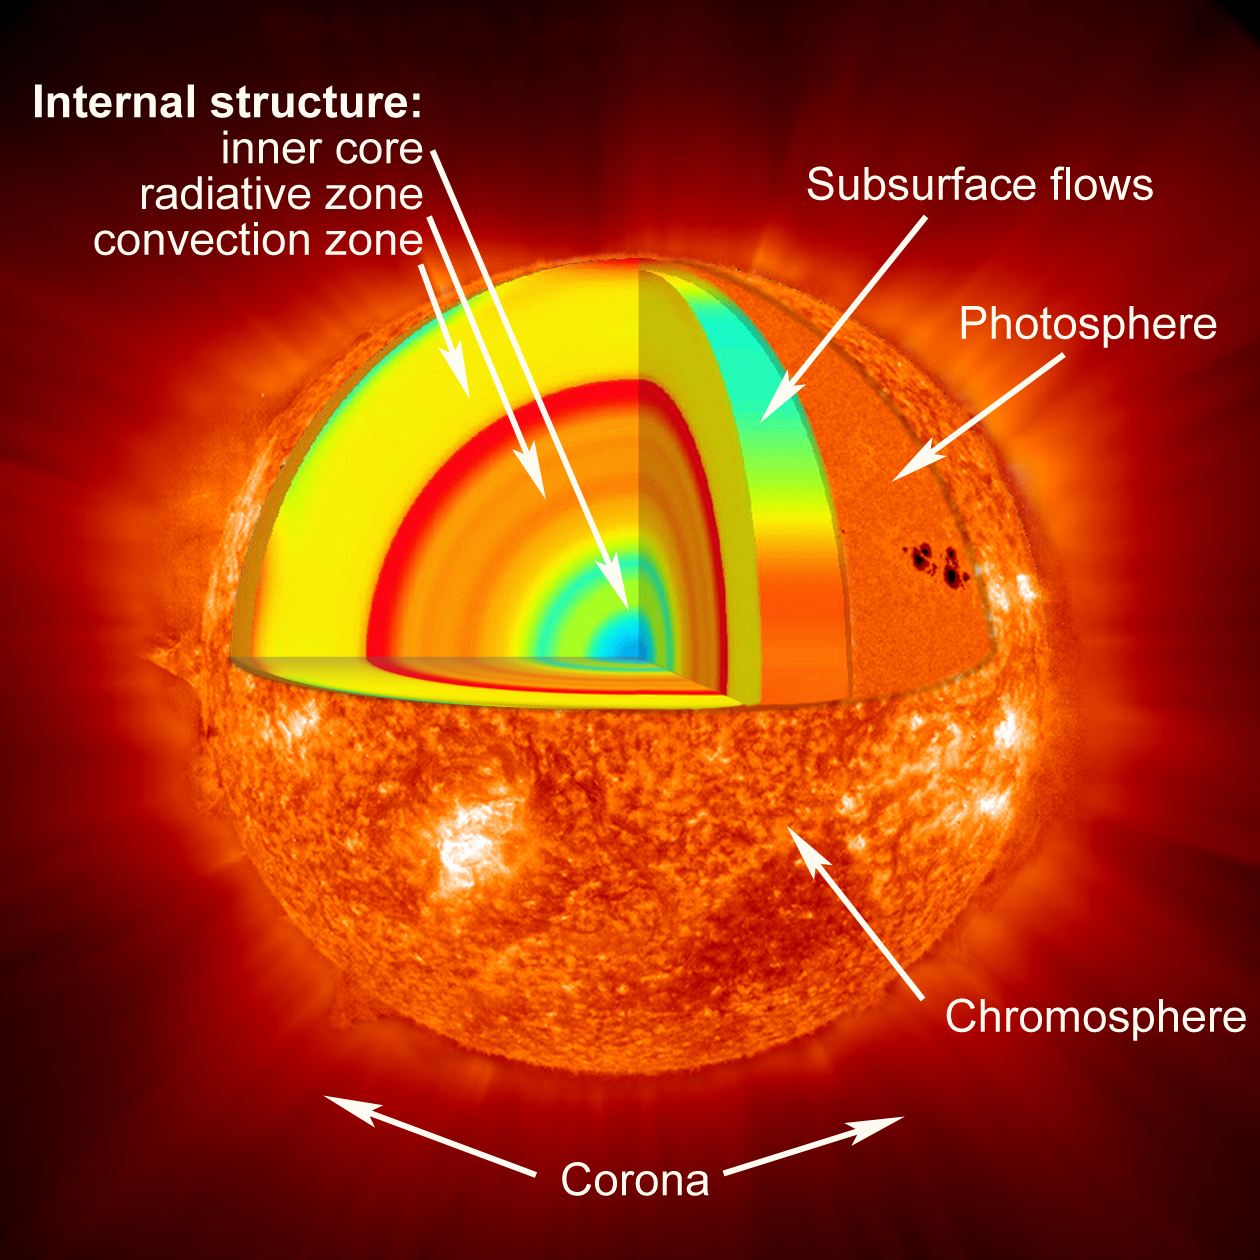
\includegraphics[width=0.5\columnwidth]{Images/Sun_interior.jpg}
%    \caption[Diagram of Sun's interior and atmospheric layers.]{Diagram of Sun's interior and atmospheric layers. Photons produced by nuclear fusion in the core transfer energy outwards through the radiative zone to ~0.7 R$_{\odot}$. At this point, convection becomes the main form of energy transport. The visible surface of the Sun is known as the photosphere and marks the boundary between the interior and the atmosphere. The solar atmosphere consists of three layers, the chromosphere, the transition region (not shown) and the corona.}
%    \label{fig:Sun}
%\end{figure}

\subsection{The Chromosphere}
In traditional plane-parallel models, the Chromosphere extends to $\sim 2000$ km above the photosphere. Its name is derived from the Greek word for colour, $\chi \rho \omega \mu \alpha$ (\textit{chroma}), in reference to the red coloured rim visible during solar eclipses. This red colour originates from the dominant Hydrogen-$\alpha$ (H$\alpha$) transition at 656.3 nm. Temperatures in the chromosphere show a decrease with distance to a local minimum of $\sim 4400$ K at $\sim 500$ km above the photosphere. The temperature then rises again to a maximum of $\sim 20,000$ K at its upper boundary. These temperatures are low enough that most of the hydrogen in the chromosphere remains neutral. 

The chromosphere exhibits numerous structures and dynamics often observed in emission lines such as H$\alpha$, the Ca II H and K lines and the Lyman-$\alpha$ transition of Hydrogen. The most prominent structural features of the quiet chromosphere include the chromospheric network on the disk and small, almost ubiquitous, jets of plasma known as spicules on the limb. The chromospheric network forms along the boundaries of supergranular cells where magnetic fields are concentrated. The magnetic field strength in the network can reach hundreds of millitesla although the average field strength of the chromosphere is $\sim 3$~mT \citep{McLean1985}.

% have been observed and are theorised to be a contributor to coronal temperatures.
% These are almost all due to the flux emergence of magnetic field in the chromosphere as evidenced by the supergranular structure. S

\subsection{The Transition Region}
The transition region occurs between the chromosphere and corona. Rather than a geometric layer, it is more accurate to consider the transition region as the region where the temperature rapidly increases (over distances as short as $\sim 100$ km) from $\sim 20,000$K to $\sim 0.8$ MK. Because the pressure remains approximately constant over this distance, the electron number density drops dramatically as is shown in Figure \ref{fig:corona_temp}. The transition region is also the part of the solar atmosphere where plasma changes from being partially ionised and collisionally dominated to fully ionised and collisionless. Network structures are also visible in low transition region images and are generally larger than those of the chromosphere, suggesting an expansion of magnetic flux tubes with height. However, the network completely disappears in higher altitude images hence, the magnetic field structure transitions from being ordered in the chromosphere to being extremely complex in the corona \citep{Tian2017}. Emission from the transition region is predominantly in the ultraviolet and extreme ultraviolet.

\subsection{The Corona}
The outermost layer of the solar atmosphere is called the corona. It contains hot, tenuous, inhomogeneous and time varying plasma which extends from the top of the transition region into interplanetary space.
%which displays a number of interesting phenomena thought to be governed by its complex magnetic field. The corona begins $\sim 2500$ km above the photosphere after a layer in the Sun's atmosphere known as the transition region, where electron density decreases and temperature increases dramatically (Figure \ref{fig:corona_temp}). 
The electron density in the corona ranges from $10^{9} \mbox{ cm}^{-3}$ at the base to $10^{6} \mbox{ cm}^{-3}$ at distances of 1 R$_{\odot}$ from the solar surface. Densities vary throughout the corona. Sparse, underdense regions at the base of the corona known as coronal holes exhibit densities of $\sim ( 0.5 - 1.0) \times 10^8 \mbox{ cm}^{-3}$ whereas areas of high magnetic activity known as active regions have electron densities of $\sim 2 \times 10^9 \mbox{ cm}^{-3}$. Active regions are the coronal counter part to sunspots and are best seen in EUV images of the Sun. The complex magnetic fields in active regions drive many of the solar phenomena such as solar flares and coronal mass ejections (CMEs).
 %Certain areas in the corona however, exhibit electron densities approximately an order of magnitude greater than the ``quiet Sun". Theses areas of high electron densities ar 

Observing the white light corona is done with a number of ground-based and space-based instruments called coronographs, that emulate the effect of a total eclipse. The Large Angle and Spectrometric Coronagraph \citep[LASCO;][]{Brueckner1995} on board the Solar and Heliospheric Observatory (SOHO) is one such instrument and allows the corona to be observed from distances of 2-32 R$_\odot$. The corona is also observed in extreme ultraviolet (EUV) lines, soft X-rays and at radio wavelengths. Observations at various wavelengths show a plethora of structure in the corona both on disk and on the limb that exist on varying time scales of a few minutes to a number of days. All particle acceleration events that produce radio emission of interest to this thesis occur in the solar corona. Figure \ref{fig:aia_quad} shows the corona and other layers of the solar atmosphere observed with the Atmospheric Imaging Assembly \citep[AIA;][]{Lemen2012}.

The high temperature of the corona remains one of the greatest mysteries in all of solar physics. Energetic events in the corona such as solar flares and CMEs, described in \ref{subsec:sf} and \ref{subsec:CMEs}, are observed across the electromagnetic spectrum. They are studied in order to understand how particles are accelerated, how energy is released and ultimately, why the corona has such an unaccountably high temperature.

% have a diagnostic in radio spectra. This PhD focuses on studying these radio diagnostics at their highest temporal and spatial resolutions to date.
\begin{figure}[ht]
\centering
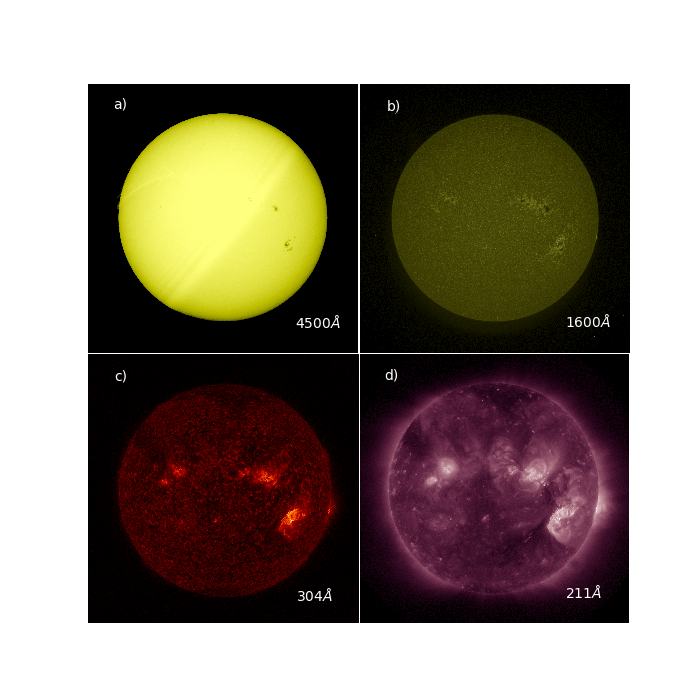
\includegraphics[width=0.8\columnwidth]{pm_aia_quad.png}
\caption[The solar atmosphere at different wavelengths.]{The Sun observed with AIA in four different wavelengths. Panel a shows the photosphere at 4500{\AA}, a group of sunspots is visible towards the southwestern limb of the sun. Panel b shows the chromosphere at 1600{\AA} and exhibits the chromospheric network. Panel c shows the upper chromosphere and transition region at 304{\AA}. Panel d shows the upper corona at 211{\AA} the active region is noticeable as the bright region in the same location as the sunspot group as in panel a.}
\label{fig:aia_quad}
\end{figure}

\section{Solar Flares}
\label{subsec:sf}
Solar flares are massive releases of magnetic energy commonly believed to be due to a reconfiguration in the complicated magnetic field structure in an active region.  They are some of the most energetic events in the solar system, releasing $\sim 10^{25}$ J of energy over a matter of minutes. Flares are observed across the electromagnetic spectrum from radio waves to $\gamma$ rays with energies $> 10$ MeV. They are classified by the amount of X-ray flux (W m$^{-2}$) detected by the Geostationary Operational Environmental Satellite (GOES) 1-8 {\AA} band on a logarithmic scale as being A, B, C, M or X class with A being the lowest flux ($10^{-8} \mbox{ W m}^{-2}$) and X the highest ($10^{-4} \mbox{ W m}^{-2}$). Each class is further subdivided into a linear scale.
A timeseries of X-ray flux from a solar flare is often called a lightcurve and has three characteristic phases; a pre-flare phase which shows X-ray flux associated with the active region where the flare occurs, an impulsive phase showing a sharp rise in X-ray flux corresponding to accelerated particles colliding with the solar surface, and a gradual decay phase where plasma heated by the flare gradually cools back to its pre-flare state. Figure \ref{fig:GOES_Xclass} shows a GOES light curve of the X9 class flare that occurred on 10 September 2017 and the three flare phases described above.

\begin{figure}[ht]
    \centering
    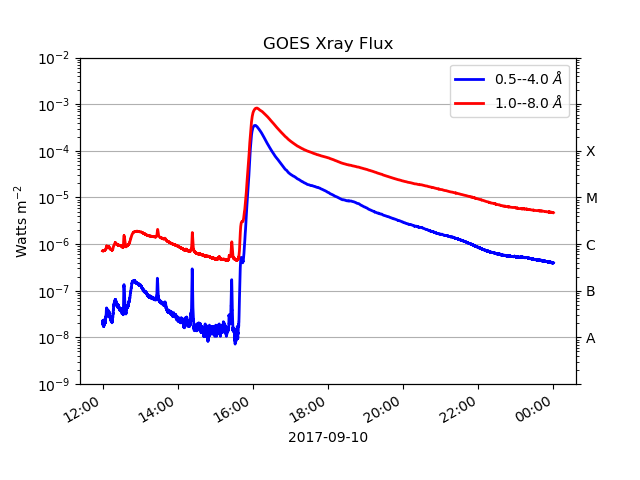
\includegraphics[width=\columnwidth]{Images/GOES_Xclass.png}
    \caption[GOES lightcurve for X9 class flare on 10 September 2017.]{The GOES lightcurve of the X9 flare that occurred on 10 September 2017. The x axis indicates the time of day on 10 September 2017 while the y axes show the X-ray flux in Wm$^{-2}$ and the flare classification. The red curve shows the 1-8 {\AA} channel by which the flare is classified while the blue curve shows the 0.5-4 {\AA} band. The three characteristic phases of a solar flare are clearly displayed here. The pre-flare phase before $\sim$ 16:00 UTC, the impulsive phase indicated by the sharp rise in flux and the gradual decay phase where X-ray flux gradually returns to the pre-flare level.}
    \label{fig:GOES_Xclass}
\end{figure}
During solar flares, magnetic structures known as coronal loops fill with hot plasma and begin to emit in soft X-rays. At the same time, electrons are accelerated towards the solar surface where their energy is converted to hard X-rays in the collision via bremsstrahlung. 

\section{Coronal Mass Ejections (CMEs)}
\label{subsec:CMEs}
In certain magnetic reconnection events, plasma suspended in a magnetic flux rope erupts from the corona into the heliosphere, the volume around the Sun where the interplanetary medium is dominated by particles flowing outward from the Sun. These eruption events are known as coronal mass ejections and accelerate 10$^{15}$ g of charged particles at typical speeds of up to $\sim 2500 \mbox{ km s}^{-1}$ \citep{Gopalswamy2000}. A ``textbook" CME structure consists of a bright front that surrounds a dark cavity and a bright central core. CMEs are observed using coronographs as they are much fainter than the solar disk. An example of a CME observed using the LASCO C2 corona with a field of view from 1.5 R$_\odot$ to 6 R$_\odot$ can be seen in Figure \ref{fig:CME}. Ejected material from a CME can interact with the Earth's magnetosphere and are known to have caused adverse effects including satellite communication disruption, radio blackouts, wide spread power outages and large inaccuracies in GPS postions \citep{Eastwood2017}. CMEs can travel faster than local Alfv\'{e}n speed in the corona leading to a shock which can accelerate particles. 

\begin{figure}[ht]
    \centering
    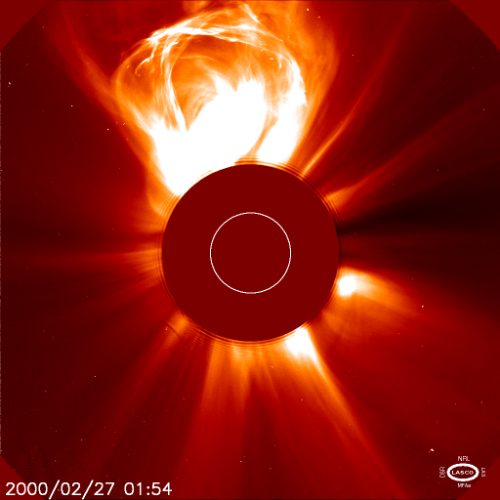
\includegraphics[width=0.75\columnwidth]{Images/LASCO_C2_CME.jpg}
    \caption[CME observed with the LASCO C2 coronograph on 27 February 2000.]{A coronal mass ejection (CME) observed with the LASCO C2 coronograph on 27 February 2000. The area covered by the coronograph is shown in the red disk in the centre of the image and the white circle represents the solar disk. The bright feature in the top of the image is the CME while less bright structures known as streamers are also seen.  }
    \label{fig:CME}
\end{figure}

\section{Solar Radio Bursts}
\label{sec:solar_radio_bursts}
In 1942 while Britain was monitoring radar signals for the signs of enemy aircraft, a strong, noise like and highly variable signal was noticed by radar operators. Upon investigation it was found that this jamming was in fact radio emission from the Sun. The discovery of this radio emission being associated with a major solar flare was kept secret until after the war and was published by \cite{Appleton1946}.
Since then the field of solar radio astronomy has flourished and significant advancements in both instrumentation and theory have occurred. Worldwide, radio interferometers such as the LOw Frequency ARray \cite[LOFAR;][]{VanHaarlem2013} and the Murchison Widefield Array \citep[MWA;][]{Lonsdale2009} have been built while next generation interferometers like the Square Kilometre Array \citep[SKA;][]{McMullin2020} are slowly being brought online. These telescopes offer a dramatic improvement on the spectral resolution and imaging capability of those that were first used to study solar radio emission.

Solar radio emission often comes in the form of bursts of varying time scales. These were initially classified into three types by \cite{Wild1950b} with a fourth and fifth type being discovered by \cite{Boischot1957} and \cite{Wild1959} respectively. A wealth of other fine structure radio bursts are also observed, predominantly found in radio storms such as S bursts, drift pairs and stria \citep{McConnell1980,Melrose1982,NelsonandMelrose1985}. 
The fine structure of these bursts can often reveal information about small-scale turbulence in the corona \citep{Reid2021}.
Figure \ref{fig:burst_cartoon} shows a schematic of the five ``classic" types of solar radio burst. A brief description of some solar radio phenomena is given below.
\begin{figure}[ht]
    \centering
    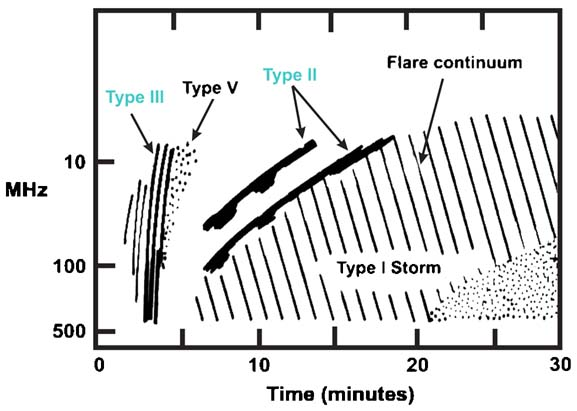
\includegraphics[width=0.75\columnwidth]{Images/Burst_cartoon.jpg}
    \caption[Cartoon of type I-V radio bursts.]{A cartoon of type I-V radio bursts. The x axis shows the time scale of the various bursts which can range from less than 1 minute to greater than 10 minutes. The y axis shows the typical frequency range of the bursts. The different drift rates of the different burst types are apparent. Image from \cite{Cliver2009}.}
    \label{fig:burst_cartoon}
\end{figure}
\paragraph{Type I bursts}
Type I emission can appear as bursts and/or a continuum originating from ``storm centres" that are associated with active regions. Type I storms can last for many days. Emission from type I bursts is highly circularly polarised in the o-mode (whereby light is circularly polarised in the opposite direction as electrons gyrating about a magnetic field line) and is also particularly directional with an increase in intensity as active regions rotate to the centre of the disk. Unlike type II or III bursts, they do not exhibit a harmonic structure \citep{McLean1985}.
\paragraph{Type II bursts}
Type II radio bursts are a form of radio emission seen from the Sun and are identified by a slow ($\sim 0.1$~MHz~s$^{-1}$) drift to lower frequencies in dynamic spectra. The frequency drift can be used to find the velocity of the shock causing a burst if the electron number density as a function of height is known. The velocities of type II bursts are often found to be $\sim 1000 \mbox{ km s}^{-1}$, which is faster than the Alfv\'{e}n velocity in the quiet corona meaning a shock must be present \citep{NelsonandMelrose1985}. Other basic properties of type II bursts include:
\begin{enumerate}
    \item Narrow bandwidths of up to $\sim 100$~MHz from initial to final frequencies.
    \item A harmonic structure of two bands with a frequency ratio slightly less than 2:1 at a fundamental, $f_p$, and harmonic, $2f_p$, frequency can be seen for most type II bursts. This structure is consistent with the idea that type II emission is due to plasma oscillations.
    \item A large number of type II bursts contain band splitting into an upper and lower band for each of the harmonics in their spectra. The cause for this splitting is not fully understood but it is commonly thought that the two bands are related to emission upstream and downstream of the MHD shock front which causes the type II burst \citep{Smerd1974,NelsonandMelrose1985, Vrsnak2002}.
    \item Herringbone structure. Approximately 20\% of type II bursts show a herringbone structure of rapidly drifting emission spikes shooting out of the ``backbone" of the main frequency drift to higher and lower frequencies. These herringbones are thought to be due to electron beams being accelerated at the associated shock for the type II burst \citep{Mann1995}. While the backbone is poorly polarised, the herringbones have been found to be quite strongly, $\sim 70\%$, polarised. The level of polarisation of herringbones determined by \cite{Suzuki1980} are similar to those of type III bursts. They suggest that this is evidence that herringbone structure is due to plasma emission from accelerated electron beams such as in the case of type III bursts. 
    \item Starting emission frequencies of the order of a few 100~MHz ending at frequencies above 20~MHz. This being said, type II burst with starting frequencies of $\sim 100$ kHz have also been observed. 
    These lower frequency bursts are thought to be due to interplanetary shocks whereas higher frequency bursts are considered to be from shocks in the low corona.
    \item Typical durations of 5-15 minutes. type II bursts that occur after a flare do so with a delay ranging from 2-20 minutes. Bursts with shorter durations generally have higher starting frequencies. %Timing and duration    
\end{enumerate}
 
Based on these and a number of other properties discussed in greater detail by \cite{NelsonandMelrose1985}, type II radio bursts can be used as indicators for MHD shocks in the solar corona. Observational proof of frequency varying inversely with time in the solar wind, consistent with radiation being generated at $f_p$ and $2f_p$ directly upstream from a CME-driven shock, was found by \cite{Reiner1997} and solidifies this argument.
\paragraph{Type III burst}
Observations of type III radio bursts (and their sub-categories) are of particular interest to this thesis and, as such, are described in Section \ref{sec:typeIII}.
\paragraph{Type IV burst}
Type IV bursts come in at least three sub-types with the general characteristic that they are of the from of broadband emission lasting for several hours. Early stationary type IV bursts (also known as the flare continuum) associated with the decay phase of solar flares, late stationary bursts which appear similar to type I emission, and moving type IV bursts which exhibit a smooth, wide-band spectrum \citep{McLean1985}.
\paragraph{Type V burst}
The last of the broadband emission bursts, type V radio bursts typically have a duration of 1-3 minutes and appear as an afterglow from type III bursts. Type V emission is strictly less than 150~MHz and is accepted that it results from electrons that generate a type III burst and become trapped in a closed magnetic loop in the corona \citep{McLean1985}.

\paragraph{Fine Structure: S bursts} 
S bursts, initially called Fast Drift Storm (FDS) bursts, were first observed at the Culgoora Solar Observatory in 1967 \citep{Ellis1969} They were later renamed by \cite{McConnell1980} who likened them to Jovian S bursts. They have a narrow bandwidth of the order of 0.03~MHz and a drift rate of 1-2~MHz~s$^{-1}$ and durations much less than 1s. \cite{McConnell1980} also concluded that S bursts are radiated at either the plasma frequency or its harmonic in a manner similar to type III bursts but that the implications of S burst fine structure and coronal scattering can only be defined once it is determined which harmonic of the plasma frequency they are radiated at. \cite{Melnik2010} propose a model of S bursts being generated by coalescence of fast magnetosonic waves with Langmuir waves which agrees well with the analysis of \cite{Clarke2019}. Modern observations of S bursts, such as those conducted using LOFAR's tied-array imaging mode \citep{Morosan2015}, can give greater insight into the spectral and temporal variability of S bursts and what this might mean for the environment they are generated in.
\\
\\The spatial extent and fine spectral structure of type III radio bursts are the main focus of this thesis. In Section \ref{sec:typeIII} below I outline the physical characteristics of type III bursts and their subcategories.

\subsection{Type III Bursts}
\label{sec:typeIII} 
Type III bursts are possibly the most useful radio burst for studying properties of plasma in the corona. As we shall see, they offer a remote measurement of the plasma density of the region where they are emitted. This allows us to probe the solar corona plasma using any of the many radio telescopes on Earth dedicated to solar radiophysics \citep[e.g.][]{Benz2004}.
\cite{Reid2014} review the observational properties of type III bursts which are repeated in brief here. The defining characteristic of type III bursts is a drift from high to low frequencies in a dynamic spectrum. The drift rates for type III bursts are typically quite fast, of the order of $\sim$ 10~MHz~s$^{-1}$ depending on the frequency. The frequency drift rate, $df/dt$, has been found to have various relations with frequency \citep{Reid2014} but most agree that $df/dt \propto f^{\alpha}$, where $\alpha$ ranges in the literature from $\sim 1$ to $\sim 2.7$. 

\cite{Ginzburg1958} proposed that type III bursts are emitted at the plasma frequency,
\begin{equation}\label{eq:1}
    \omega_{p}^2 = \frac{N_e e^2}{m_e \varepsilon_0}
\end{equation}
where $N_e$ is the number density of electrons, $m_e$ is the electron mass, $e$ is the electron charge and $\varepsilon_0$ is the permittivity of free space. A more detailed description of the plasma emission process is given in Section \ref{sec:plasma_emission}.
Although Eq. \ref{eq:1} is relatively simple, it contains an important relationship in plasma physics. Namely, the plasma frequency is proportional to the square root of the electron density. This means that plasmas at higher electron densities will oscillate at higher frequencies than those of lower densities. The drift in type III bursts, which are emitted at $\omega_p$, is therefore an indication of the emission source moving from an area of high electron density to low density, i.e. from the lower to the upper corona. Using a model of electron density in the corona such as the \cite{Newkirk1961} model, it can be inferred that the exciter of type III bursts has a speed of $\sim 0.3$~c.

\begin{figure}[ht]
    \centering
    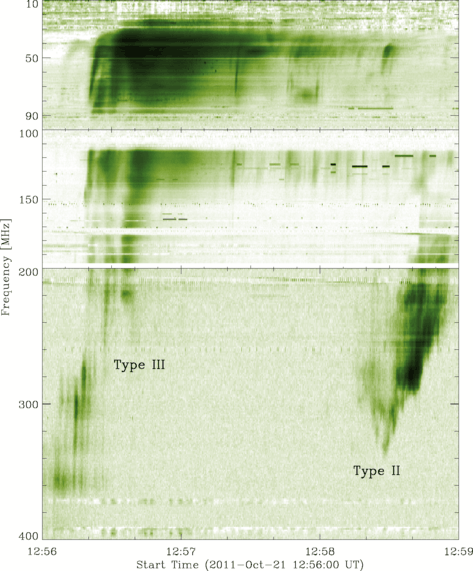
\includegraphics[width=0.75\columnwidth]{Images/Pietro_typeIII.png}
    \caption[A number of type III bursts observed by \cite{Zucca2012} on 21 October 2011.]{A number of type III bursts observed by \cite{Zucca2012} on 21 October 2011. The x axis gives the time on 21 October 2011 while the y axis shows the frequency in MHz. A number of type III bursts extend to frequencies below 200~MHz. A type II burst can be seen between 140 and 330~MHz later in the day.}
    \label{fig:bursts}
\end{figure}

Type III bursts are observed to be in two bands, a fundamental and harmonic band that are emitted at $\omega_p$ and $2 \omega_p$ respectively. Both bands exhibit the same frequency drift although the flux of the harmonic band is usually less than that of the fundamental band \citep{Wild1954a, McLean1985}. The process of plasma emitting radio frequencies at $\omega_p$ and $2 \omega_p$ will be explained in more detail in Chapter \ref{chap:theory}. 
Figure \ref{fig:bursts} shows type III radio bursts below 400~MHz observed by \cite{Zucca2012}. A type II burst was also observed between 140 and 330~MHz and exhibits a much slower frequency drift than the type III bursts. A type III storm can be seen below 200~MHz. This is when type III emission is continuous over the span of large time scales and can last days. Type III bursts come in a number of subcategories described below.

\paragraph{Reverse and bi-directional bursts.}

A typical type III burst is produced when an electron beam travels along a magnetic field line away from the Sun to areas of lower density. If, instead, electrons travel towards the Sun to areas of higher density a reversed frequency drift is observed. Bursts where both the regular and reverse drifts can be seen simultaneously are bi-directional bursts \citep{Reid2014}.

\paragraph{Type IIIb bursts.}

\begin{figure}[ht]
\centering
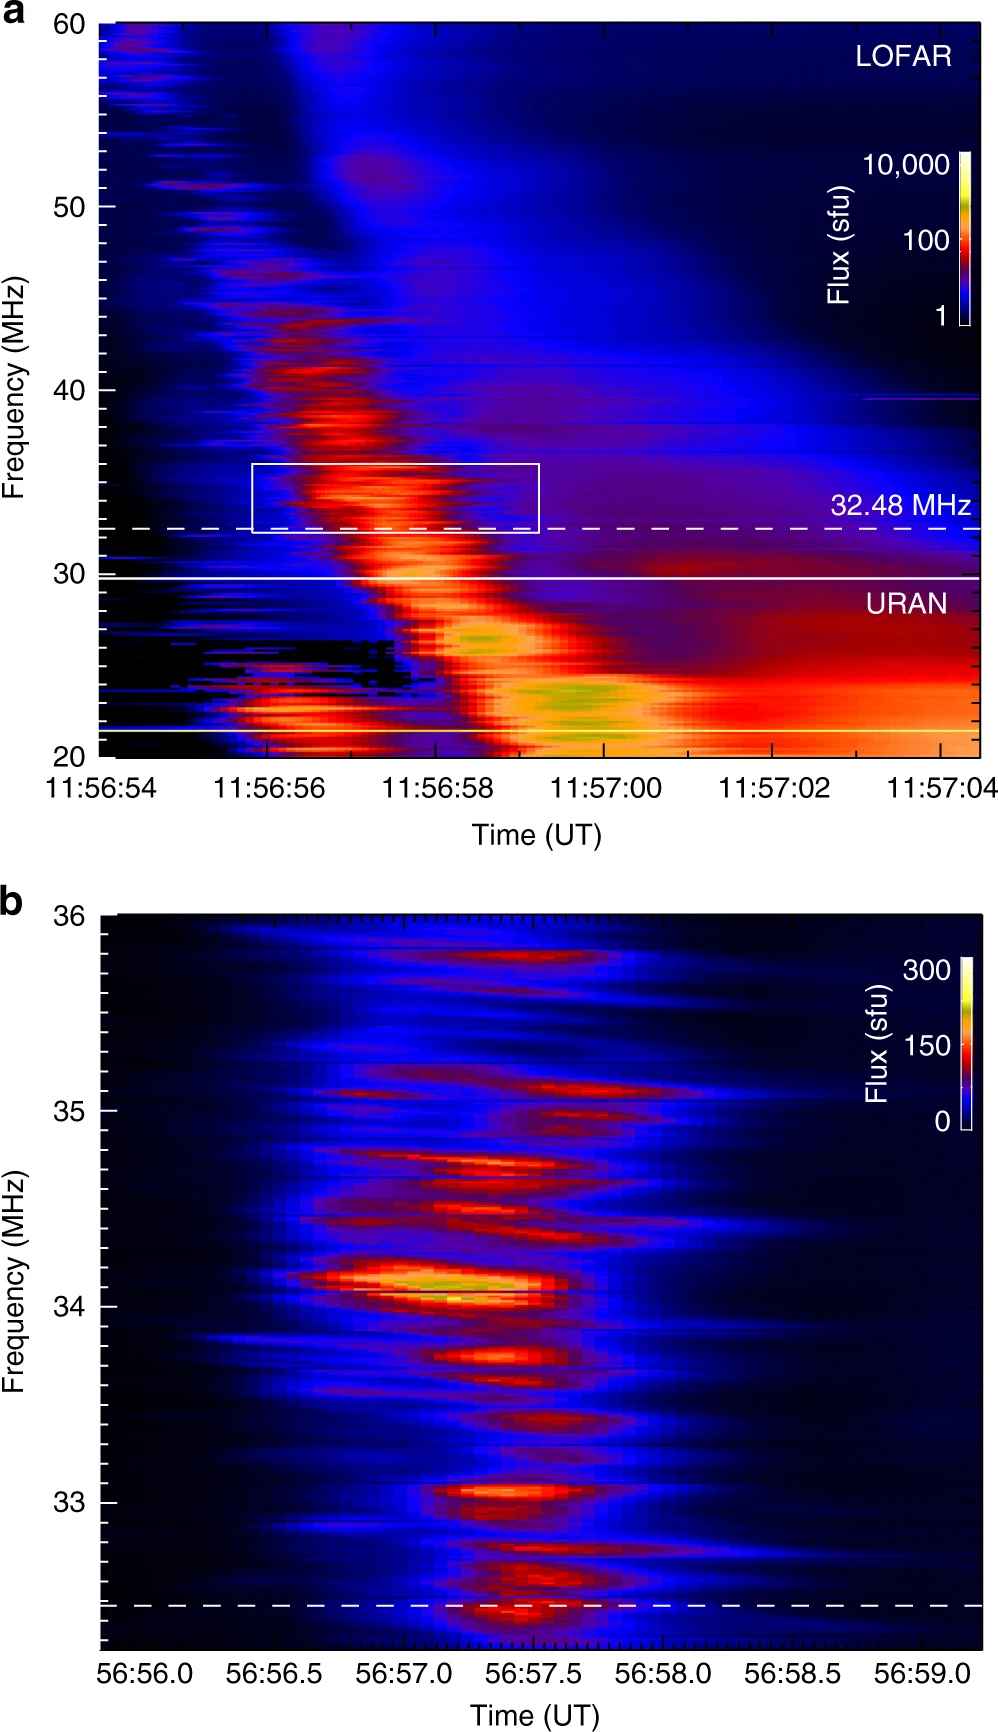
\includegraphics[width=0.5\columnwidth]{typeIIIbKontar.png}
\caption[The type IIIb radio burst from \cite{Kontar2017}.]{A type IIIb radio burst on 16 April 2015 analysed by \cite{Kontar2017}. Panel a shows the full duration of the type IIIb. Panel b is a zoom in of the 3 second wide box in panel a.}
\label{fig:typeIIIbKontar}
\end{figure}

Fine frequency structures are sometimes seen in type III bursts. Type IIIb radio bursts are defined as a number of narrow, nearly horizontal, frequency bands called striae, or striations, in the envelope of a type III. The frequency width of an individual striae is typically 0.05~MHz \citep{McLean1985} and they have a frequency drift rate of $\lesssim 150$~kHz~s$^{-1}$, which implies a speed of 0.6~Mm~s$^{-1}$ \cite{Sharykin2018}. Figure \ref{fig:typeIIIbKontar} shows a dynamic spectrum of a type IIIb burst from \cite{Kontar2017}. Individual striae can be clearly seen in panel b of Figure \ref{fig:typeIIIbKontar}. The theory describing the origin of this fine frequency structure has recently been revisited by \cite{Reid2021} who found that the striations are due to turbulence in the corona and their drift a result of moving Langmuir waves.

\paragraph{Type U and J bursts.}

In the case where electrons are travelling along a closed magnetic field line, a turning point in the frequency drift of a type III burst can be observed. For electrons that generate radio emission down to the footpoint of the magnetic field line, a U burst is observed. A U burst can be identified as an inverted U on a dynamic spectrum. More often, electrons stop generating radio emission as they travel back down the magnetic field line so only the turning point in frequency drift is visible in dynamic spectra. These are known as J type bursts. U and J bursts are far less common than type III bursts, despite the similar number of open and closed magnetic field lines along which electron beams can propagate. The reason for this proposed by \cite{Reid2017} is that the length of these closed loops is not long enough for the electron beam to become unstable to Langmuir waves.

\paragraph*{} The study of type III bursts offers an insight into the process of Langmuir wave generation in the solar corona and as such are an important tool in understanding the physics of coronal plasma \citep{Reid2014}. However, the effects of radio wave propagation from the source to the observer through the corona must but understood before inferences can be drawn from observations. 

\subsection{Low Frequency Radio Wave Scattering}

Spectral analysis of short temporal radio bursts with small bandwidths at $\sim 30$~MHz suggests that source sizes in the corona are of the order $\lesssim 1$ arcmin \citep{McConnell1980, Kontar2017}. Radio images of the Sun at metric and decametric wavelengths have yet to reveal this level of spatial structure. This was mostly due to the limitations of angular resolution of radio telescopes at the time. 
Observations with modern interferometers at these frequencies however, still have not observed spatial structure at these scales. The suggestion that there is a fundamental limit imposed upon the level of resolution obtainable by scattering of radio waves in a turbulent corona \citep{Bastian1994} has re-emerged in recent years \citep{Thejappa2007,Thejappa2008,Kontar2017,Kontar2019}. 

The development of scattering theory stems from \cite{Chandrasekhar1952} description of light scattered by a thin screen and will be outlined further in Chapter \ref{chap:theory}. The implementation of this theory into computational modelling has also seen considerable development since the first ray tracing experiments by \cite{Fokker1965}. \cite{Steinberg1971} built upon this by including the effect of spherical refraction through the corona and were able to obtain the time response of a scattered pulse source.

Both \cite{Fokker1965} and \cite{Steinberg1971} followed from \cite{Chandrasekhar1952} and assumed density inhomogeneities in the corona had a Gaussian power spectrum. However, it is now known that this assumption is incorrect. \cite{Bastian1994} provides a review of the work by \cite{Coles1989} and others to determine the shape of density inhomogeneity power spectrum. At large scales, greater than a few hundred kilometres, the spectrum is well described with a power law index of 11/3, which agrees with the Kolmogorov description of turbulence \citep{Kolmogorov1941}. For scales smaller than these but greater than a few kilometres, the spectrum becomes shallower and is better described with a power law index of $\sim 3$. Finally, on the smallest scales less than a few kilometres the spectrum steepens again. This steepening has been interpreted as the scale at which energy is dissipated by turbulence. \cite{Coles1989} also found that this inner scale increases with heliocentric distance. \cite{Bastian1994} expanded on this description of the density inhomogeneity power spectrum and investigated the angular broadening of radio waves sources at centimetre wavelengths.

The latest development in the modelling of radio wave scattering is by \cite{Kontar2019}. Rather than using the small scattering angle approximation of previous work, \cite{Kontar2019} build on the work of \cite{Arzner1999} and \cite{Bian2019}. In this approach, the effect of anisotropic density inhomogeneities is treated as photon diffusion in momentum space and the Hamiltonian equations for photon position and momentum can be solved iteratively to trace a photon's path. This allows for a continuous transition from weak to strong scattering, whereas previous work is limited to regime of small angle scattering. 

Understanding radio wave propagation effects, in particular scattering, is important because they affect all observations made at radio wavelengths. Radio wave scattering has been shown to depend on the relative level of density fluctuations in the corona and as such, offers a chance to learn about its turbulent nature. By classifying the power spectral density of these fluctuations it may be possible to gain an understanding of the turbulent processes that transport energy to the microscopic scales and result in the heating of the corona. 

\section{Thesis Outline}
The high spatial, temporal and spectral resolution of modern radio interferometers such as LOFAR and the launch of new space missions including Parker Solar Probe \citep[PSP;][]{Fox2016} and Solar Orbiter \citep{Muller2020} has ushered in a new age of solar radio observations. By developing a computational backend and using a unique method for fitting interferometric visibilities, this thesis has furthered the capability of an international LOFAR station and extracted value from existing interferometric observations. This thesis outlines how such developments have improved our knowledge of radio wave propagation in the solar corona using observations at some of the highest spatial, spectral and temporal resolutions available. In Chapter \ref{chap:theory} I outline the relevant background theory for the work presented in this thesis. Chapter \ref{chap:instrumentation} will describe the instrumentation used throughout this thesis, namely LOFAR, and the mathematical background for interferometric imagining. 

The REALtime Transient Acquistion backend (REALTA), is a seven node computer cluster designed to record and analyse the raw beamformed data from international LOFAR stations in real-time. The development of REALTA for solar and a myriad of other observations formed a key part of this work. Chapter \ref{chap:REALTA} describes the hardware and software of REALTA and showcases some first light observations.
 
The study of radio wave scattering in the solar corona has undergone a renaissance in recent years both in terms of computational modelling and observations. Chapter \ref{chap:measuring_source_sizes} will describe how, for the first time, LOFAR visibilities were fitted directly to determine the size and position of a type IIIb burst. This lead to a more subtle understanding of the root mean squared fluctuations of electron density in the solar corona, the key parameter necessary to quantify the effect of scattering. 

In order to accurately compare between models of the solar corona, in Chapter \ref{chap:observations_vs_theory} I present 29 type III radio bursts and determine their size and position using the visibility fitting technique with a Markov Chain Monte Carlo optimization. The results of this show that type III bursts exhibit an intrinsic source size greater than the size of a point source that has been scattered and highlights discrepancies between observations and computational modelling.

Chapter \ref{chap:future} includes a discussion on the future work that can be carried out from the foundations of this thesis. It outlines the necessary further studies needed to further our knowledge of radio wave scattering and how to utilise even higher temporal resolution observations of the radio sun. Chapter \ref{chap:future} will also contain a summary and conclusion of the work presented in this thesis.


%!TEX root = ../main.tex
\doublespacing
\chapter{Theoretical Background}
\label{chap:theory}
The following chapter describes the core concepts relevant to this thesis in more detail than Chapter \ref{chap:intro}. Here I discuss the various mechanisms for radio wave emission in the solar corona, with particular emphasis on the plasma emission process. I will also give an introduction to the mathematical formalisms of radio interferometry.
\section{Introductory Concepts in Plasma Physics}
Plasma was the name given by Langmuir to the new, exotic type of matter he was studying in the 1920s. It is essentially an ionized gas that exhibits quasi-neutrality on a macroscopic scale. Maxwell-Boltzman distributions.
\subsection{Plasma Frequency}
\section{Radio Emission Mechanisms in the Solar Corona}
\subsection{Bremstrahlung}
\subsection{Gyroemission}
\subsection{ECMI}
\subsection{Plasma Emission}
\section{Plasma Emission}
\label{sec:plasma}
In 1942 while Britain was on the look out for radar signals of enemy aircraft, a strong, noise like and highly variable signal was noticed by radar operators. Initially it was thought that Germany had managed to learn the secret of radar and create some sort of jamming device. On further investigation it was found that this jamming was in fact radio emission from the Sun. The discovery of this radio emission being associated with a major solar flare was kept secret until after the war and was published by \cite{Appleton1946}.
Since then a number of major advancements in both instrumentation and theory have occurred. A culmination of the theory of solar radio emission is laid out in the book by \cite{McLean1985} while worldwide, a number of extraordinary radio telescopes and interferometers such as the LOw Frequency ARray \cite[LOFAR,][]{VanHaarlem2013}, the Nan\c{c}ay Radio Heliograph and the Murchison Widefield Array (MWA), to name but a few, have been built.

Solar radio emission often comes in the form of bursts of varying timescales. These were initially classified into three types by \cite{Wild1950b} with a fourth and fifth type being discovered by \cite{Boischot1957} and \cite{Wild1959} respectively. Of these, the most frequently occurring are the so called Type III radio bursts. These are short bursts that can be observed over many frequencies and are found to be associated with solar flares \citep{Malville1962}. An initial study into how they are emitted was conducted by \cite{Ginzburg1958}.% This essay examines Type III bursts and in particular describes their observed characteristics, what causes them and the plasma emission process of their generation.

%\section{Process of Forming Type III Bursts} %(This is how they're made)}
For a Type III radio burst to be emitted, an electron must generate Langmuir waves in the plasma. These Langmuir waves then go on to generate electromagnetic transverse waves by coalescing with other waves or by decaying. Theses electromagnetic waves are the radio bursts that are observed. In this section the generation of Langmuir waves and the process of plasma emission are discussed.

\subsection{Generation of Langmuir Waves}
During magnetic reconnection in a solar flare electrons are accelerated along magnetic field lines. As these beams of electrons propagate, faster electrons begin to outpace slower electrons and stationary ions in the background plasma. This leads to a second peak on the Maxwell Boltzmann distribution of velocities as seen in Figure \ref{fig:Lwavegrowth}. Energy is transferred from electrons electrons travelling at the phase velocity, $v_{\phi}$ , to Langmuir waves creating a resonance.
The positive velocity gradient of this resonance means that there are more electrons with velocity greater than $v_{\phi}$ than there are electrons with velocities less than  $v_{\phi}$ (where energy is transferred from the wave to the particles), this causes Langmuir waves to become unstable and their magnitudes to grow exponentially. Particles with velocities near $v_{\phi}$ are in resonance with the Langmuir waves and drive this instability.

This instability is alleviated by what is known as quasi-linear relaxation \citep{Melrose1987} whereby the resonant behaviour of the electrons and Langmuir waves results in a plateau in the Maxwell Boltzmann distribution rather than a second peak. It can be shown that \citep{Vedenov1963} the electron distribution function, $f(v,t)$ where $\int f(v,t) dv = n_e$, and the spectral energy index of Langmuir waves, $W(v,t)$ such that $\int W(v,t) dv = E_L$ the total energy density, can be expressed as follows \citep{Reid2014},
\begin{equation}\label{eq:dfdt}
    \frac{\partial f(v,t)}{\partial t}=\frac{4 \pi^2 e^2}{m_e^2} \frac{\partial}{\partial v} \left( \frac{W}{v} \right) \frac{\partial f(v,t)}{\partial v}
\end{equation}

\begin{equation}\label{eq:dWdt}
    \frac{\partial W(v,t)}{\partial t}= \frac{\pi \omega_p}{n_e} v^2 W \frac{\partial f(v,t)}{\partial v}
\end{equation}

Equation \ref{eq:dWdt} shows that the growth rate of Langmuir waves is proportional to $\frac{\partial f(v,t)}{\partial v}$, hence a positive gradient in the Maxwell Boltzmann distribution leads to a growth in Langmuir waves. The right hand side of Eq. \ref{eq:dfdt} has a diffusion operator $D=\frac{W}{v}$. This states that the transfer of energy from particles to waves and back leads to the distribution function being smoothed out and eventually becoming a plateau. The evolution of $f(v,t)$ and $W(v,t)$ with time is shown in Figure \ref{fig:Lwavegrowth}. Figure \ref{fig:Lwavegrowth} shows how the plateau in the distribution function and a broadening in the spectral energy density develop as time progresses.

\begin{figure}
    \centering
    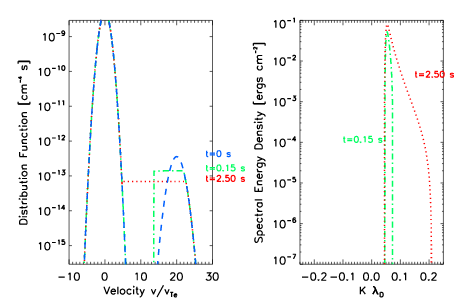
\includegraphics[width=0.75\columnwidth]{Images/L_wave_growth.png}
    \caption[Langmuir wave distriburtion function and spectral energy density.]{Left: Evolution of distribution function (normalised by the electron thermal velocity $v_{Te}=V_e$) in time. The diffusive term in \ref{eq:dfdt} causes the bump-on-tail Gaussian to turn into a plateau, thereby eliminating the instability caused by the positive velocity gradient. Right: The spectral energy density of generated Langmuir waves, x-axis normalised to the Debye length $\lambda_D=\sqrt{\frac{\epsilon_0 k_B T_e}{e^2 n_e}}$. As time passes the spectral range of Langmuir waves increases. Each panel shows successive times of t=0.15s (green, dot-dashed line) and t=2.50s (red, dotted line). \citep[Figure taken from][]{Reid2014}.} %(Figure taken from \citeauthor{Reid2014} \citeyear{Reid2014})}
    \label{fig:Lwavegrowth}
\end{figure}

\subsection{Wave-Wave Interaction}\label{Plasma Emission}
Wave-wave interaction concerns the processes by which three types of waves interact. These are: transverse (T) waves, Langmuir (L) waves and ion sound (S) waves, and have the following, respective dispersion relations,
$$ \omega=(\omega_p^2 +k^2c^2)^{\frac{1}{2}} $$
$$ \omega \cong \omega_p + \frac{3k^2V_e^2}{2 \omega_p}$$
$$ \omega = kv_s $$
where $V_e$ is the thermal velocity of electrons in the plasma, $v_s$ is the ion sound speed and $k$ is the wave vector. Only transverse waves with $\omega > \omega_p $ can escape and thus a plasma emission mechanism is a process that generates these transverse waves. 

As mentioned in Section \ref{characteristics}, Type III bursts have a harmonic structure associated with plasma emission at the plasma frequency and the second harmonic. Both of these transverse waves are formed in different three wave processes that will now be discussed.
In a plasma, due to scattering from other wave modes and ions in the plasma, a wave mode can be changed from one to the other. This is expressed in the equation 
$$ \sigma \rightleftarrows \sigma' + \sigma '' $$
where $\sigma$, $\sigma'$  and  $\sigma ''$ represent different wave modes. Conservation of energy and momentum state,
$$ \omega^{\sigma}(k)=\omega^{\sigma'}(k')+\omega^{\sigma''}(k'')$$
$$ k=k'+k''$$
where $ \omega^{\sigma}(k)$ is the frequency of a particular wave mode with the wave vector $k$. For Langmuir (L), ion sound (S) and transverse (T) wave modes the allowed processes are L+S$\rightarrow$L', L+S$\rightarrow$T,  T+S$\rightarrow$L,  T+S$\rightarrow$T' and  L+L'$\rightarrow$T. Of these L+S$\rightarrow$T,  L$\rightarrow$T+S are responsible for fundamental emission while harmonic emission is associated with the three wave process L+L'$\rightarrow$T.

Originally \cite{Ginzburg1958} considered fundamental emission to be due to Langmuir waves scattering off of thermal ions in the plasma. It is now commonly accepted that the biggest cause of fundamental emission is due to the three wave processes of a Langmuir wave coalescing with an ion sound wave generated by L$\rightarrow$L'+S or when a Langmuir wave decays into an ion sound wave and an electromagnetic transverse wave. The process L$\rightarrow$T+S can be visualised as in Figure \ref{fig:Femission}. In solar radio physics it is often assumed that $k_L \gg k_T$, knowing this and that the wave vectors must satisfy $\mathbf{k}_L \pm \mathbf{k}_s = \mathbf{k}_T$ ($+$ for L+S$\rightarrow$T , $-$ for L$\rightarrow$T+S) implies $\mathbf{k}_s \approx \mp \mathbf{k}_L$ 

\begin{figure}
\centering
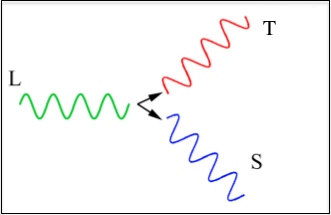
\includegraphics[width=0.5\columnwidth]{Images/Fundamental_emission_Lwaves.png}
\caption[A three wave process of fundamental plasma emission L$\rightarrow$T+S]{A three wave process of fundamental plasma emission L$\rightarrow$T+S. A Langmuir wave decaying into an ion sound wave and an electromagnetic transverse wave at the plasma frequency. (Figure adapted from Solar (interplanetary) Radio Bursts: the Generation of Radio Waves,	an oral presentation by David Malaspina at the Jean Louis Steinberg International Workshop on Solar, Heliospheric and Magnetospheric Radioastronomy, November 2017)}
\label{fig:Femission}
\end{figure}

Second harmonic emission occurs when two Langmuir waves coalesce in the process L+L'$\rightarrow$=T, shown in Figure \ref{fig:Hemission}. Conservation of momentum requires that $\mathbf{k}_L + \mathbf{k'}_L = \mathbf{k}_T$ and for second harmonic (H) generation, $k_T=k_H \approx \frac{\sqrt{3} \omega_p}{c}$. The phase speed $v_\phi$ of Langmuir waves is much less than $\frac{c}{\sqrt{3}}$ meaning that $k_L \gg k_T$ which results in $\mathbf{k}_L \approx -\mathbf{k'}_L$. This means that for a transverse wave at the second harmonic to be created, two Langmuir waves must coalesce almost exactly head on. These backward propagating Langmuir waves are generated: in the three wave processes of L+S$\rightarrow$L' and L$\rightarrow$L'+S; scattering off of thermal ions; and refraction at density inhomogeneities.
 \begin{figure}

     \centering
     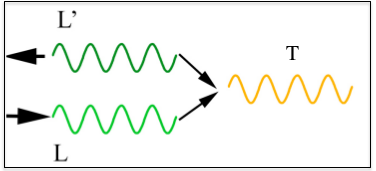
\includegraphics[width=0.5\columnwidth]{Images/Harmonic_emission_Lwaves.png}
     \caption[Three wave process of second harmonic plasma emission L+L' $\rightarrow$ T]{Three wave process of second harmonic plasma emission L+L' $\rightarrow$ T. A Langmuir wave (L) and a backwards propagating Langmuir wave (L') coalesce to form a transverse wave (T) at $2 \omega_p$. (Figure adapted from Solar (interplanetary) Radio Bursts: the Generation of Radio Waves,	an oral presentation by David Malaspina at the Jean Louis Steinberg International Workshop on Solar, Heliospheric and Magnetospheric Radioastronomy, November 2017)}
     \label{fig:Hemission}
 \end{figure}
%!TEX root = ../main.tex
\doublespacing
\chapter{Instrumentation and Interferometric Imaging}
\label{chap:instrumentation}
Solar Radio bursts in the corona can be studied in both spectra and images using observations from radio telescopes and interferometers. This chapter describes the instrumentation used throughout the work for this thesis, namely the LOw Frequency ARray (LOFAR). In order to study the spatial extent of radio bursts, a number of LOFAR stations are used together to create interferometric images.  High temporal resolution spectra can be recorded using a single LOFAR station during ``local mode". I begin with a description of the entire LOFAR array and give a detailed description of the digital signal processing pipeline of an international LOFAR station such as the Irish LOFAR station (I-LOFAR) in Birr, County Offaly. 
%Here I also describe the REALtime Transient Acquisition Backend (REALTA), which was developed to record data from I-LOFAR in real-time and perform a number of post-processing procedures. 
Finally, I outline the mathematical background for radio interferometry and give a brief description of a common deconvolution algorithm to generate interferometric images.

\section{The LOw Frequency ARray (LOFAR)}
The LOw Frequency ARray \citep[LOFAR;][]{VanHaarlem2013} is a radio interferometer located in eight countries across Europe. The majority of the LOFAR stations exist in a dense cluster in the Netherlands known as the core. There are a total of 52 LOFAR stations; 24 core stations, 14 remote stations (also in the Netherlands), and 14 international stations (spread across Europe). The planned construction of an additional international station in Italy will increase this to a total of 53 LOFAR stations. A subset of densely packed core stations known as the ``superterp" is shown in Figure \ref{fig:superterp}. Although it is not dedicated to solar observations, LOFAR is the ideal instrument with which to observer solar radio bursts in the frequency range of 10 - 240 MHz. The temporal, spectral and spatial resolution are significantly improved upon the instruments first used to observe solar radio bursts from 60 years ago and as such, has reinvigorated the study of low frequency radio emission from the solar corona. In particular, the Solar and Space Weather Key Science Project (KSP) for LOFAR have secured observational time to overlap with the perihelion passes of both Parker Solar Probe \citep[PSP;][]{Fox2016} and Solar Orbiter \citep{Muller2020}, allowing for simultaneous remote and \textit{in situ} observations of coronal plasma at distances $< 10 R_\odot$ for the first time in human history.

 
\begin{figure}[ht]
\centering
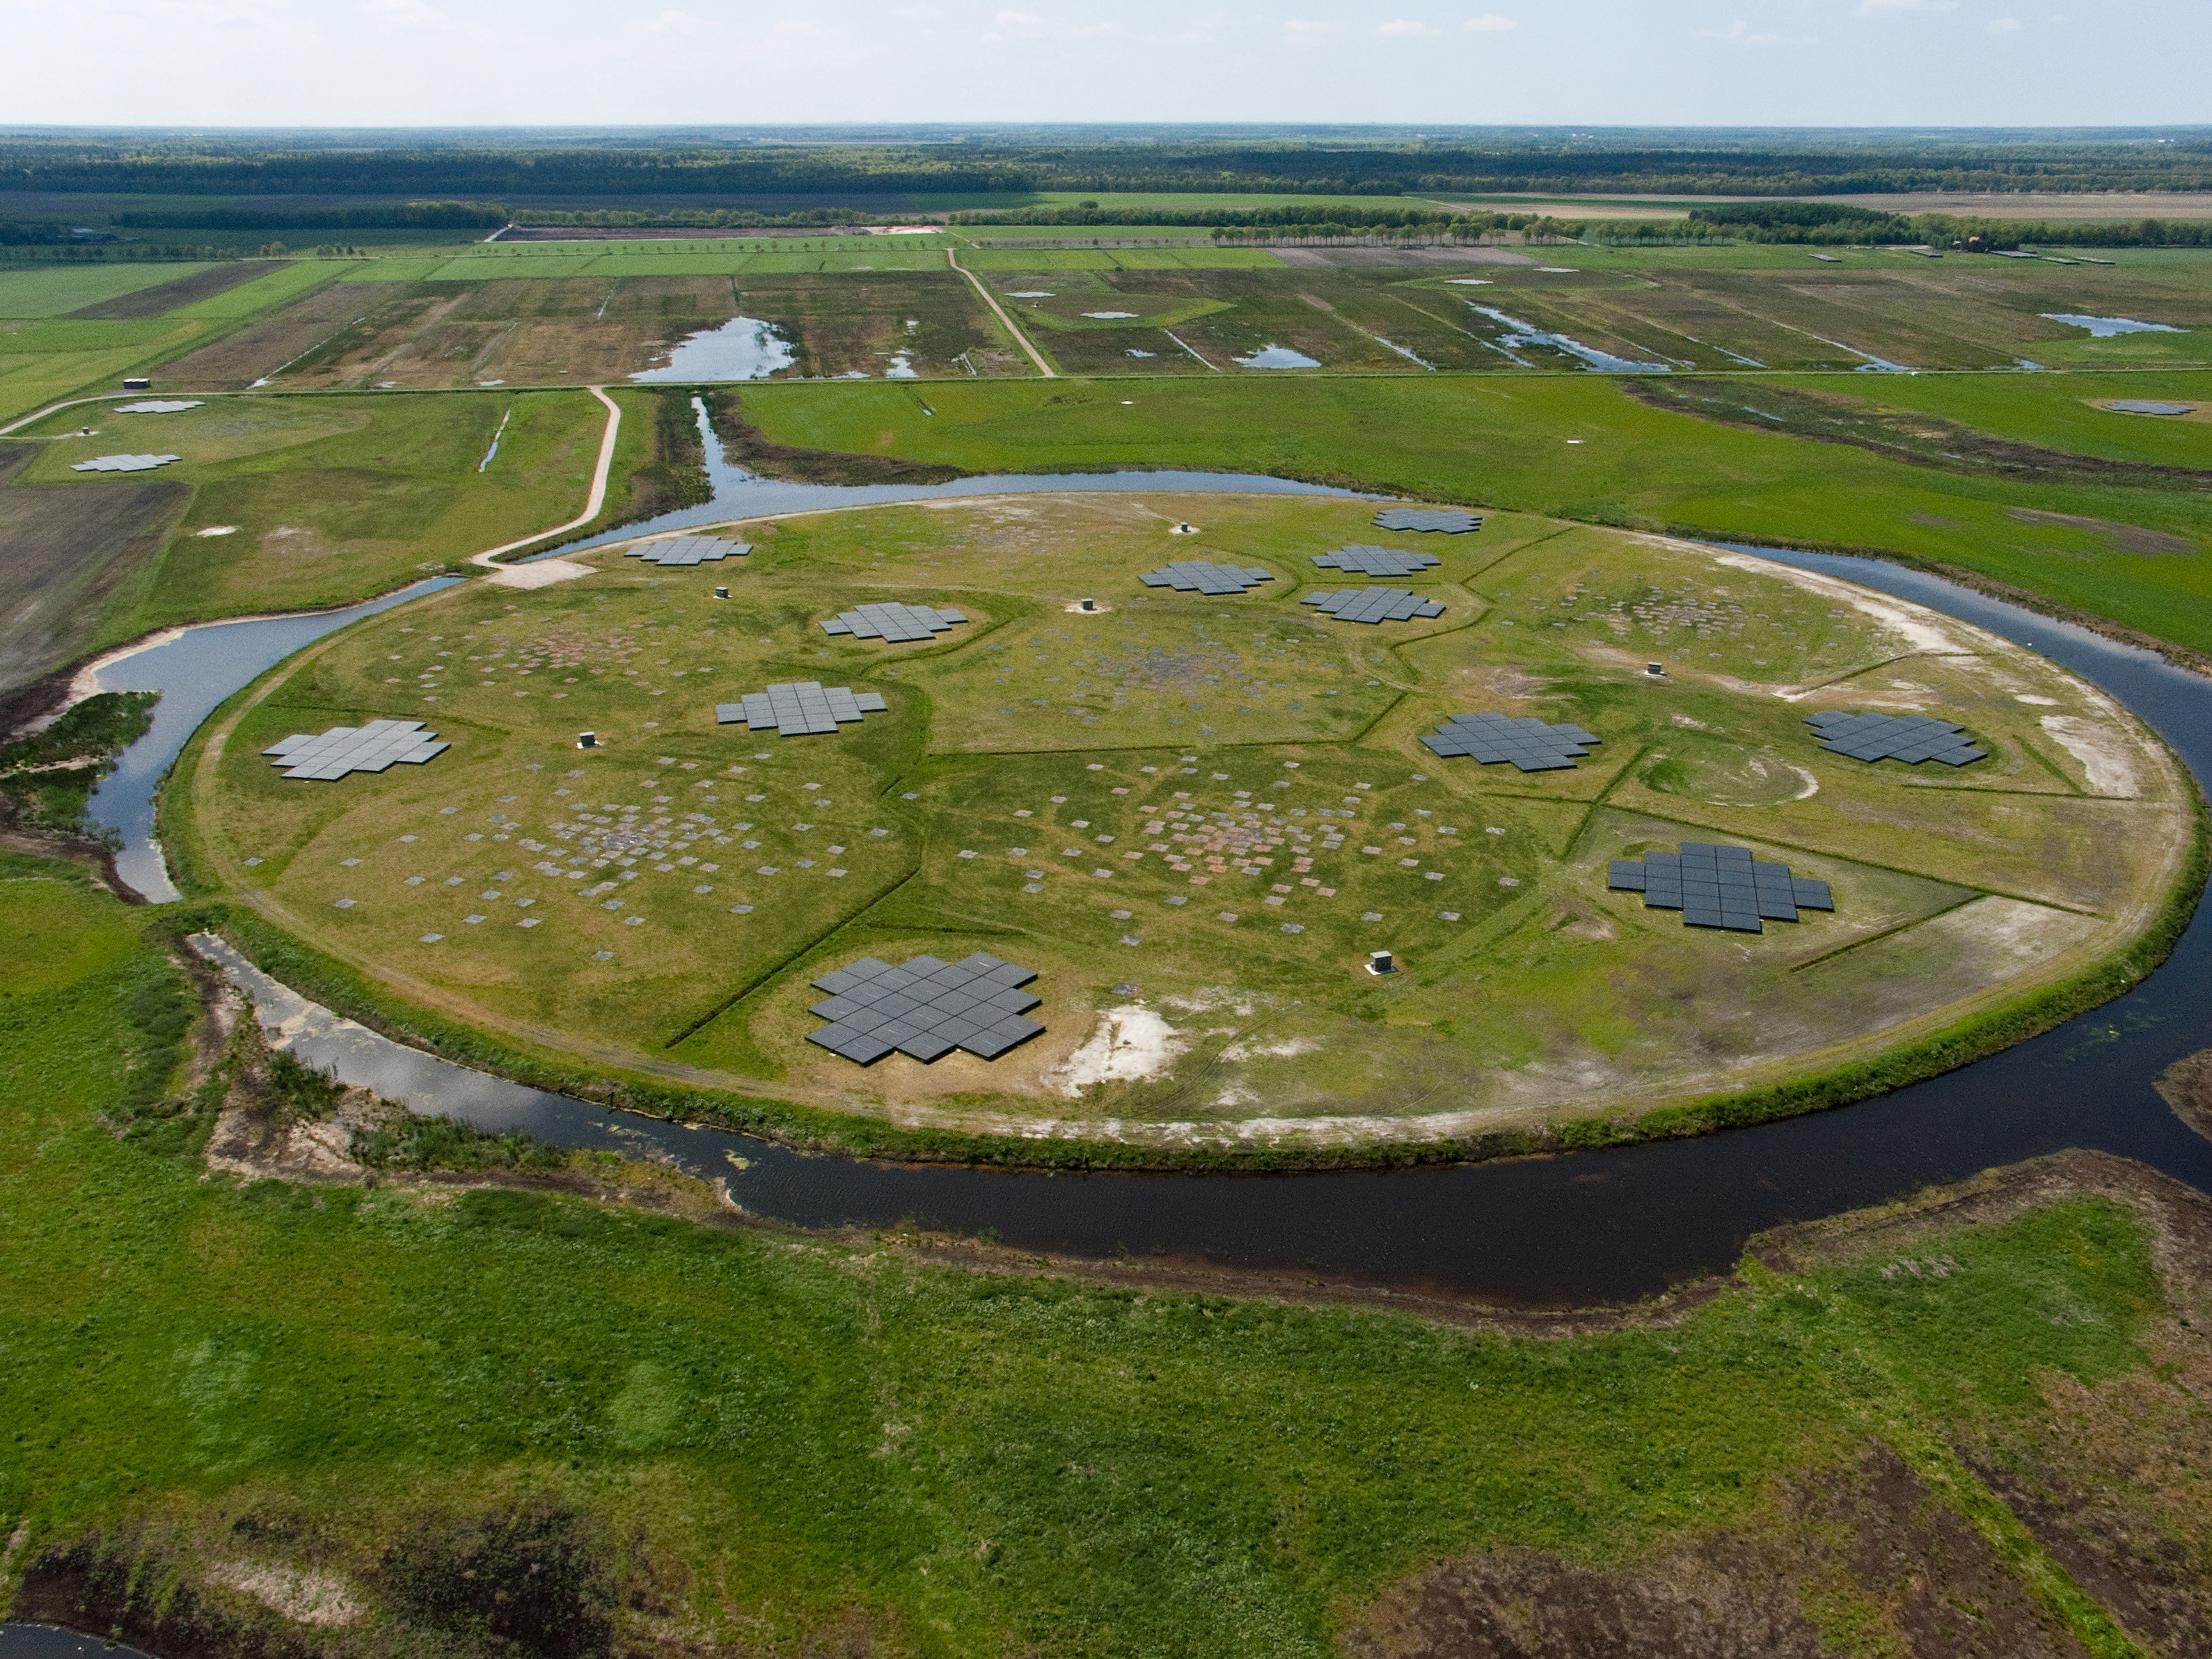
\includegraphics[width=\columnwidth]{LOFAR_Superterp.jpg}
\caption[The LOFAR superterp]{A dense collection of LOFAR core stations known as the ``superterp". Image credit ASTRON/LOFAR. The large black tiles are the HBAs while the smaller grey squares mark the locations of the LBAs.}
\label{fig:superterp}
\end{figure}
%The LOw Frequncy ARray \citep[LOFAR;][]{VanHaarlem2013} is a radio interferometric array located in across Europe. The first LOFAR core station was completed in 2008. Since then, LOFAR has continued to grow to 40 stations in the Netherlands alone with a further 14 across the rest of Europe and another station planned for completion in Italy in the near future. Along with the addition of new stations, an extensive set of software for imaging, calibration, RFI flagging and more has been written for use with data produced by LOFAR. Imaging pipelines described in \cite{VanHaarlem2013} have also been developed to further maximise the quality of the sub-arcsecond spatial resolution data LOFAR can provide with its full $\sim 2000$ km baseline.
%Every LOFAR station is connected to the CEntral Processor cluster (CEP) located in Groningen in the Netherlands by 10Gbps fibre optic cable where data is beamformed and correlated by the COrrelator and Beamformer Application for the LOFAR Telescope, a GPU based cluster designed with commercial components \citep{Broekema2018}.

The frequency bandwidth of LOFAR is split into two bands, observed with a different type of antenna, both of which can be seen in Figure \ref{fig:superterp}. The range 10 - 90 MHz is observed with the Low Band Antennas (LBAs) and the range 110 - 240 MHz is observed with the High Band Antennas (HBAs). The gap between the two bands is included to avoid observing in the FM band, which is dominated by noise from commercial radio broadcasting. The observations in Chapters \ref{chap:measuring_source_sizes} and \ref{chap:observations_vs_theory} were made using the LBAs while monitoring of solar radio activity with the I-LOFAR uses both the LBAs and HBAs simultaneously, as discussed in section \ref{sec:I-LOFAR}. I now discuss the antennas and recording process for an international LOFAR station.
% how images are made from LOFAR observations will be discussed in section \ref{sec:interferometry}.
%To observer in each band, two different antenna designs are utilised, the Low Band Antenna (LBA) for 10-90MHz and the High Band Antenna (HBA) for 110-240MHz. % In order to observe in these two bands, LOFAR uses two different antenna designs, the Low Band Antenna (LBA) for 10-90MHz and the High Band Antenna (HBA) for 110-240MHz. 
\subsection{Low Band Antenna}
The LBA is a cross dipole antenna in an inverted V shape consisting of two lengths of orthogonal copper wire. This enables measurements from two linear polarisations in the X and Y direction. LBAs are oriented such that the X polarisation is in the Northeast to Southwest direction while the Y polarisation runs Northwest to Southeast. Each wire is connected to a low noise amplifier inside of a radio frequency interference (RFI) shielded mould on top of a 1.7m PVC pipe. The pipe is kept upright under tension from the wires which are attached to the ground with synthetic rubber straps and polyester rope. The LBA is placed on top of a steel ground plane made out of concrete reinforcement rods, which acts as a reflector for radio light. Figure \ref{fig:LBA} shows LBAs at I-LOFAR. The low noise amplifiers receive power over two coaxial cables, which also carry signals measured from the LBA.

\begin{figure}[ht]
\centering
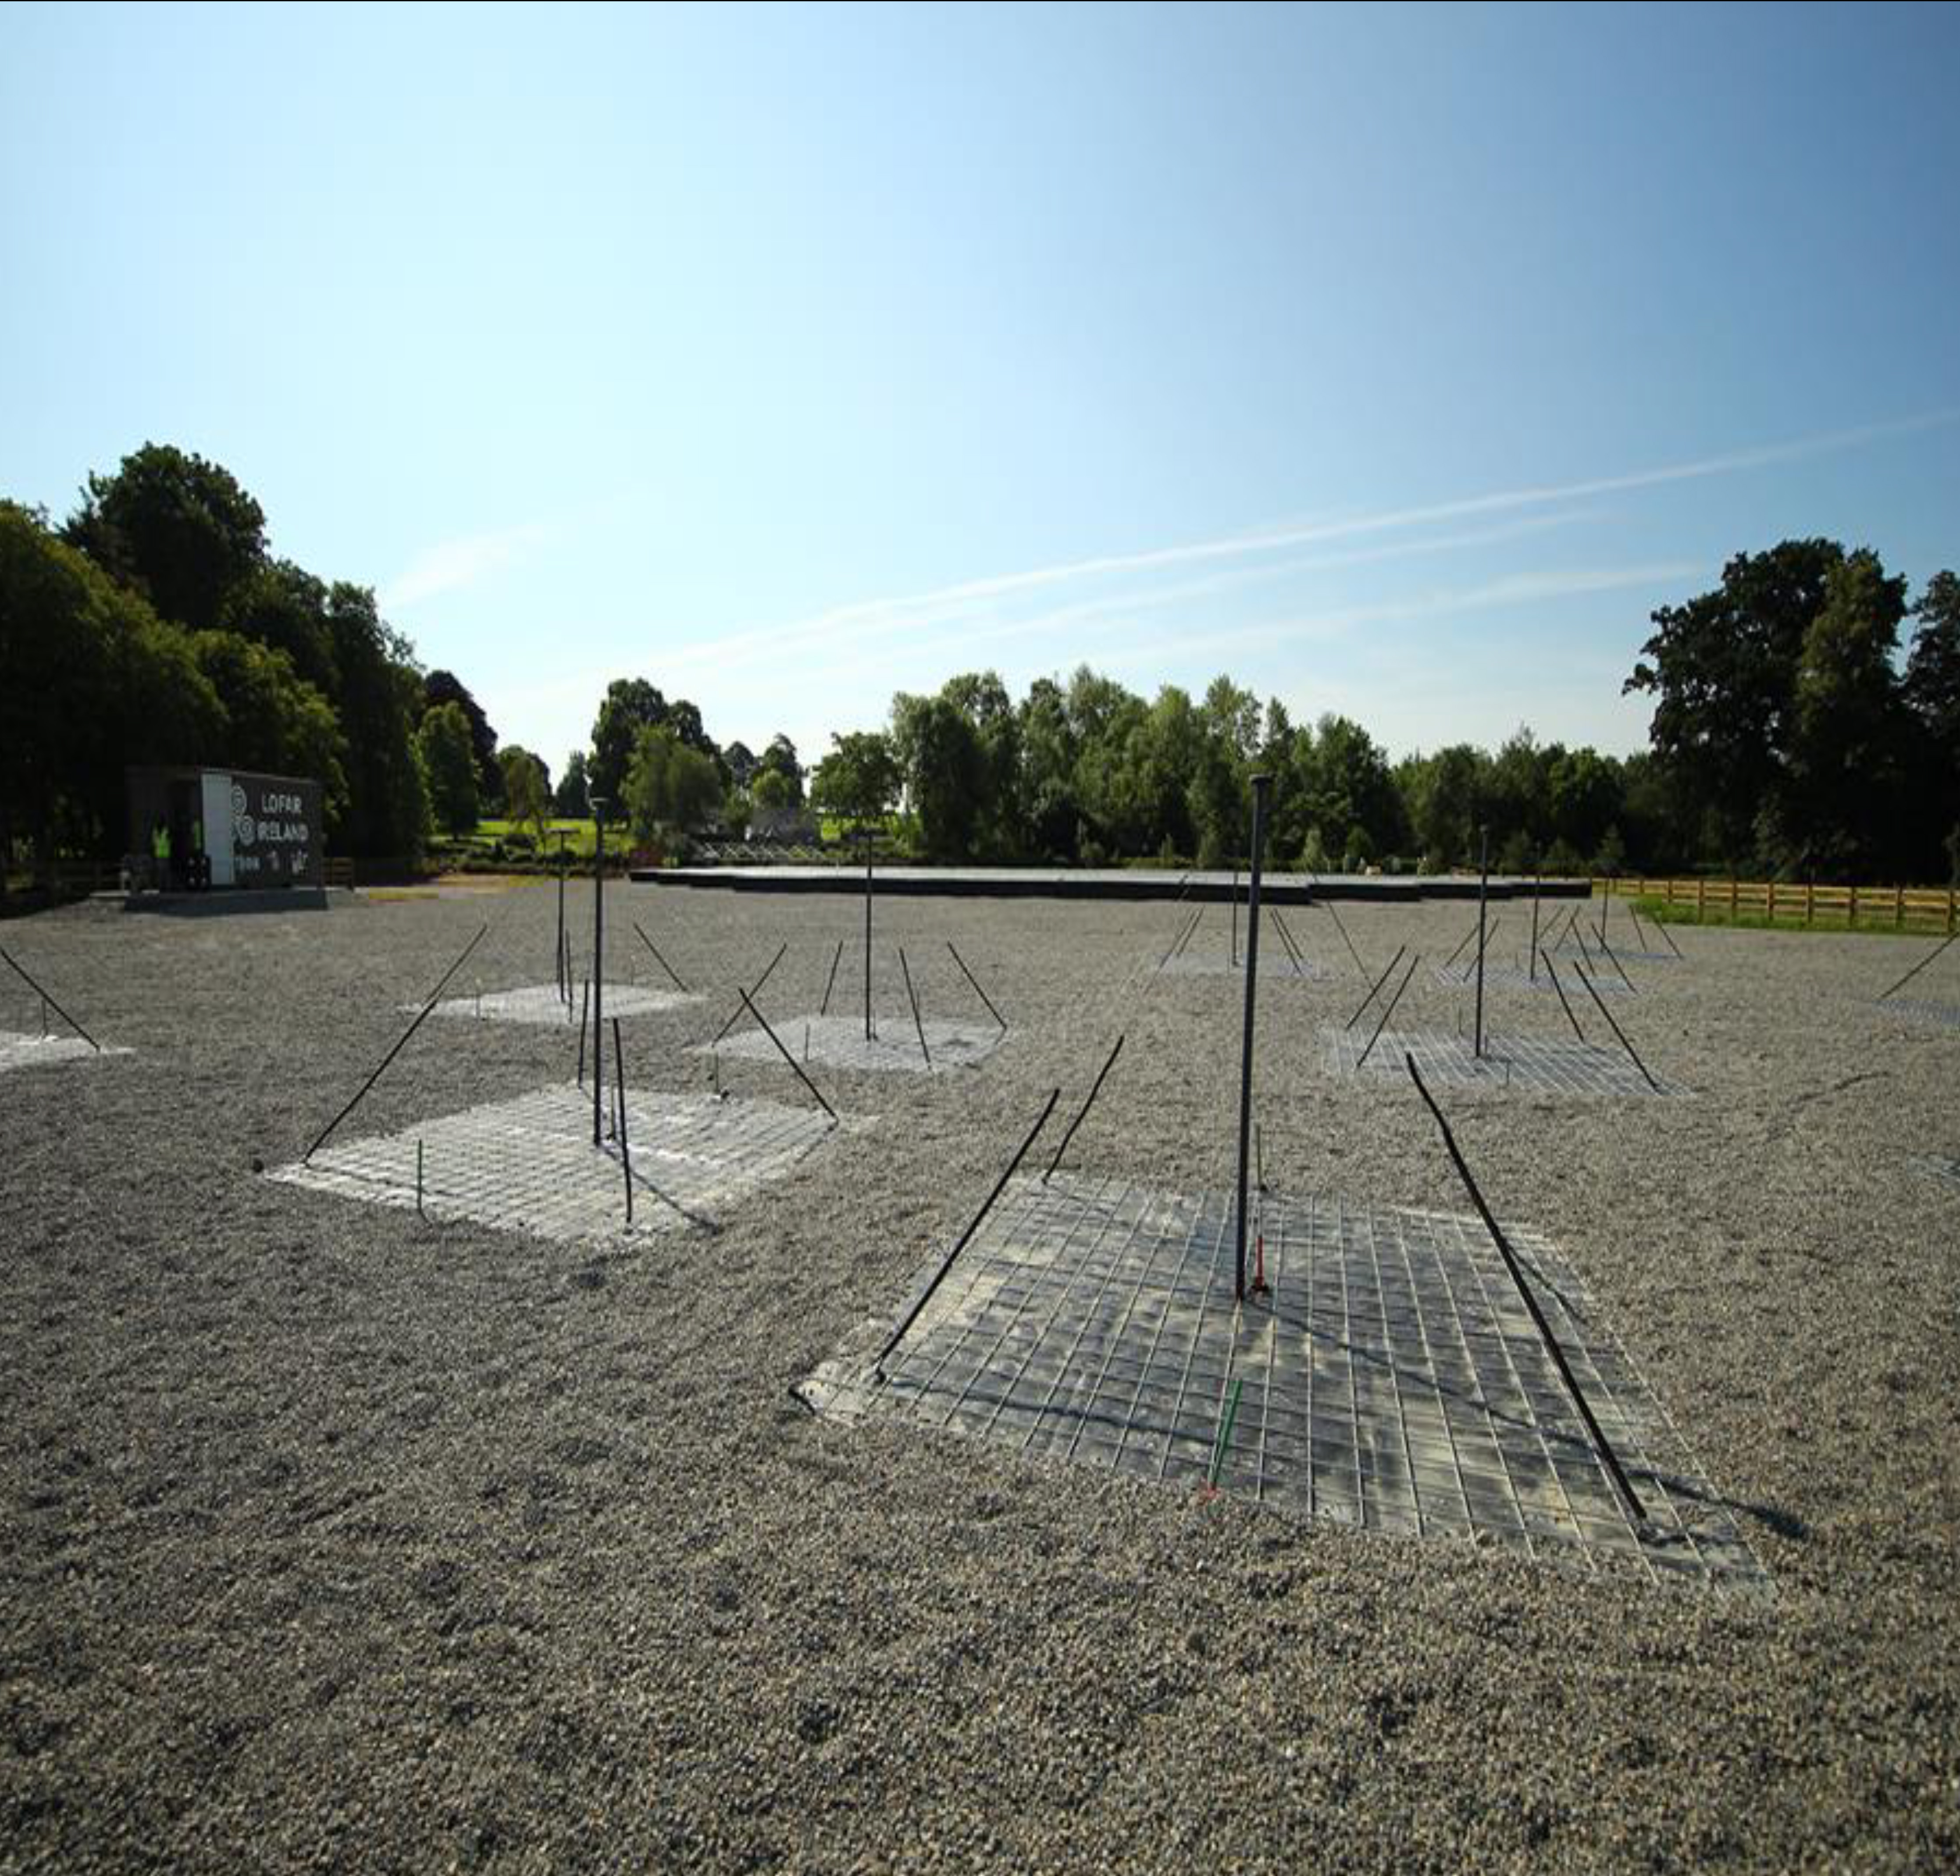
\includegraphics[width=\columnwidth]{LBA.jpg}
\caption[Low Band Antennas at I-LOFAR]{Low Band Antennas on a rare sunny day at I-LOFAR. The dipoles are connected via coaxial cable down through the PVC pipe to the station container in the background.}
\label{fig:LBA}
\end{figure}

Each arm of the dipole is 1.38m long which results in a 52MHz resonance peak however, due to the impedance of the amplifier this is increased to 58MHz. A typical LBA power spectrum showing this resonance peak can be seen in Figure \ref{fig:LBA_power_spec}.

\begin{figure}[ht]
    \centering
    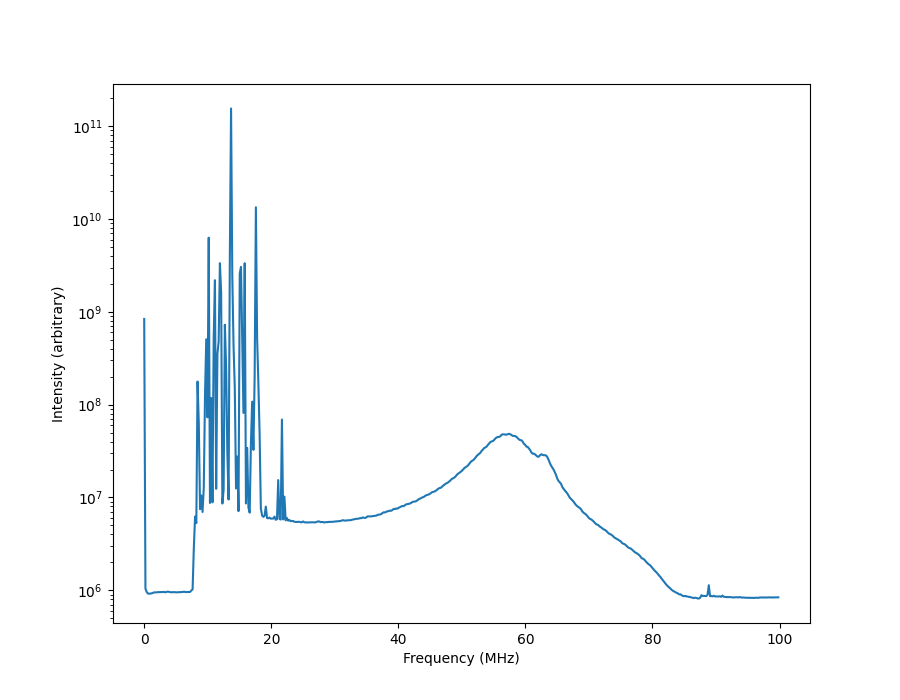
\includegraphics[width=\columnwidth]{lba_powerspec.png}
    \caption[Typical power spectrum for an LBA.]{Typical power spectrum for an LBA. The peak at 58 MHz is determined by the length of the dipole arms and the impedance of the low noise amplifier. The `knee' in the spectrum at $\sim 63$ MHz is due to the wires being turned up at the ends.}
    \label{fig:LBA_power_spec}
\end{figure}

\begin{figure}[ht]
\centering
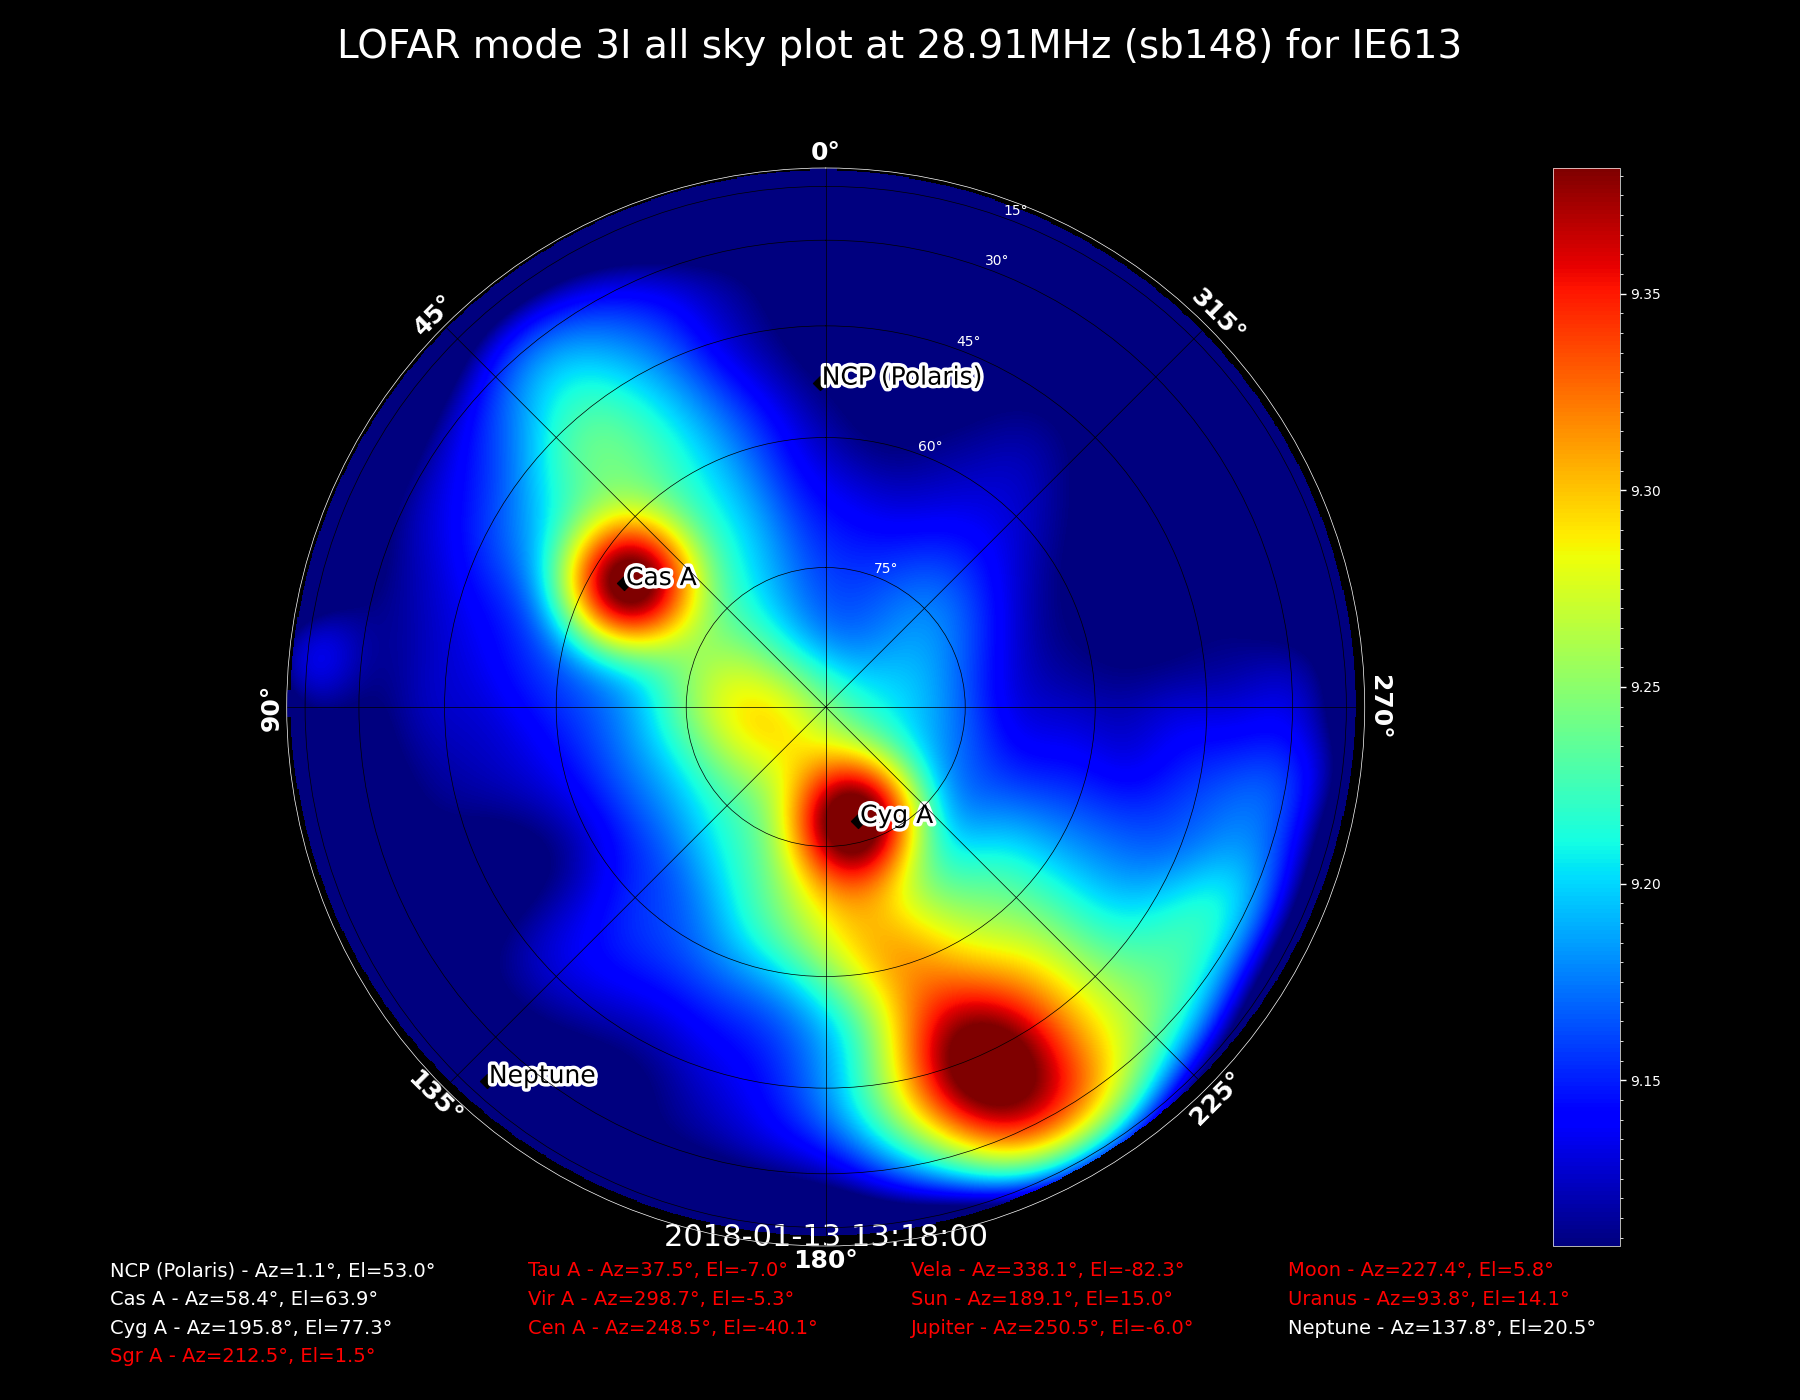
\includegraphics[width=\columnwidth]{lba_allsky.png}
\caption[A total intensity all sky image taken with I-LOFAR LBAs.]{An all-sky image taken with I-LOFAR LBAs at 28.91 MHz. The positions of Cassiopeia A and Cygnus A are shown to line up well with the brightest parts of the image.}
\label{fig:LBA_allsky}
\end{figure}

 %and digital beamforming techniques can by used  to form a beam at any part of the sky within seconds.
%This pipe is anchored to a metal ground plane made out of steel commonly used in concrete reinforcement by two 1.38m copper wires which act as a cross dipole antenna, thus allowing both X and Y polarisations to be measured. The simple structure of the LBA means that there is a resonance peak at $\sim 58$MHz.
\subsection{High Band Antenna}
The spectrum above the FM band is observed by the HBA. In order to reduce system noise, the HBA design is drastically different to the simple design of the LBA. One HBA is a 5m x 5m tile consisting of a 4 $\times$ 4 array of 16 bow-tie cross dipole antenna elements supported in an expanded polystyrene structure. The HBA sits on top of a 5cm $\times$ 5cm wire mesh ground plane, which acts as a reflector to radio waves at these higher frequencies. The HBA tile is encased in two overlapping polypropylene foil layers in order to protect it from the weather. Figure \ref{fig:HBA} shows a fully assembled HBA tile before the tile lid is placed. The 4 $\times$ 4 grid of antenna elements expanded polystyrene structure is clearly seen.

\begin{figure}[ht]
\centering
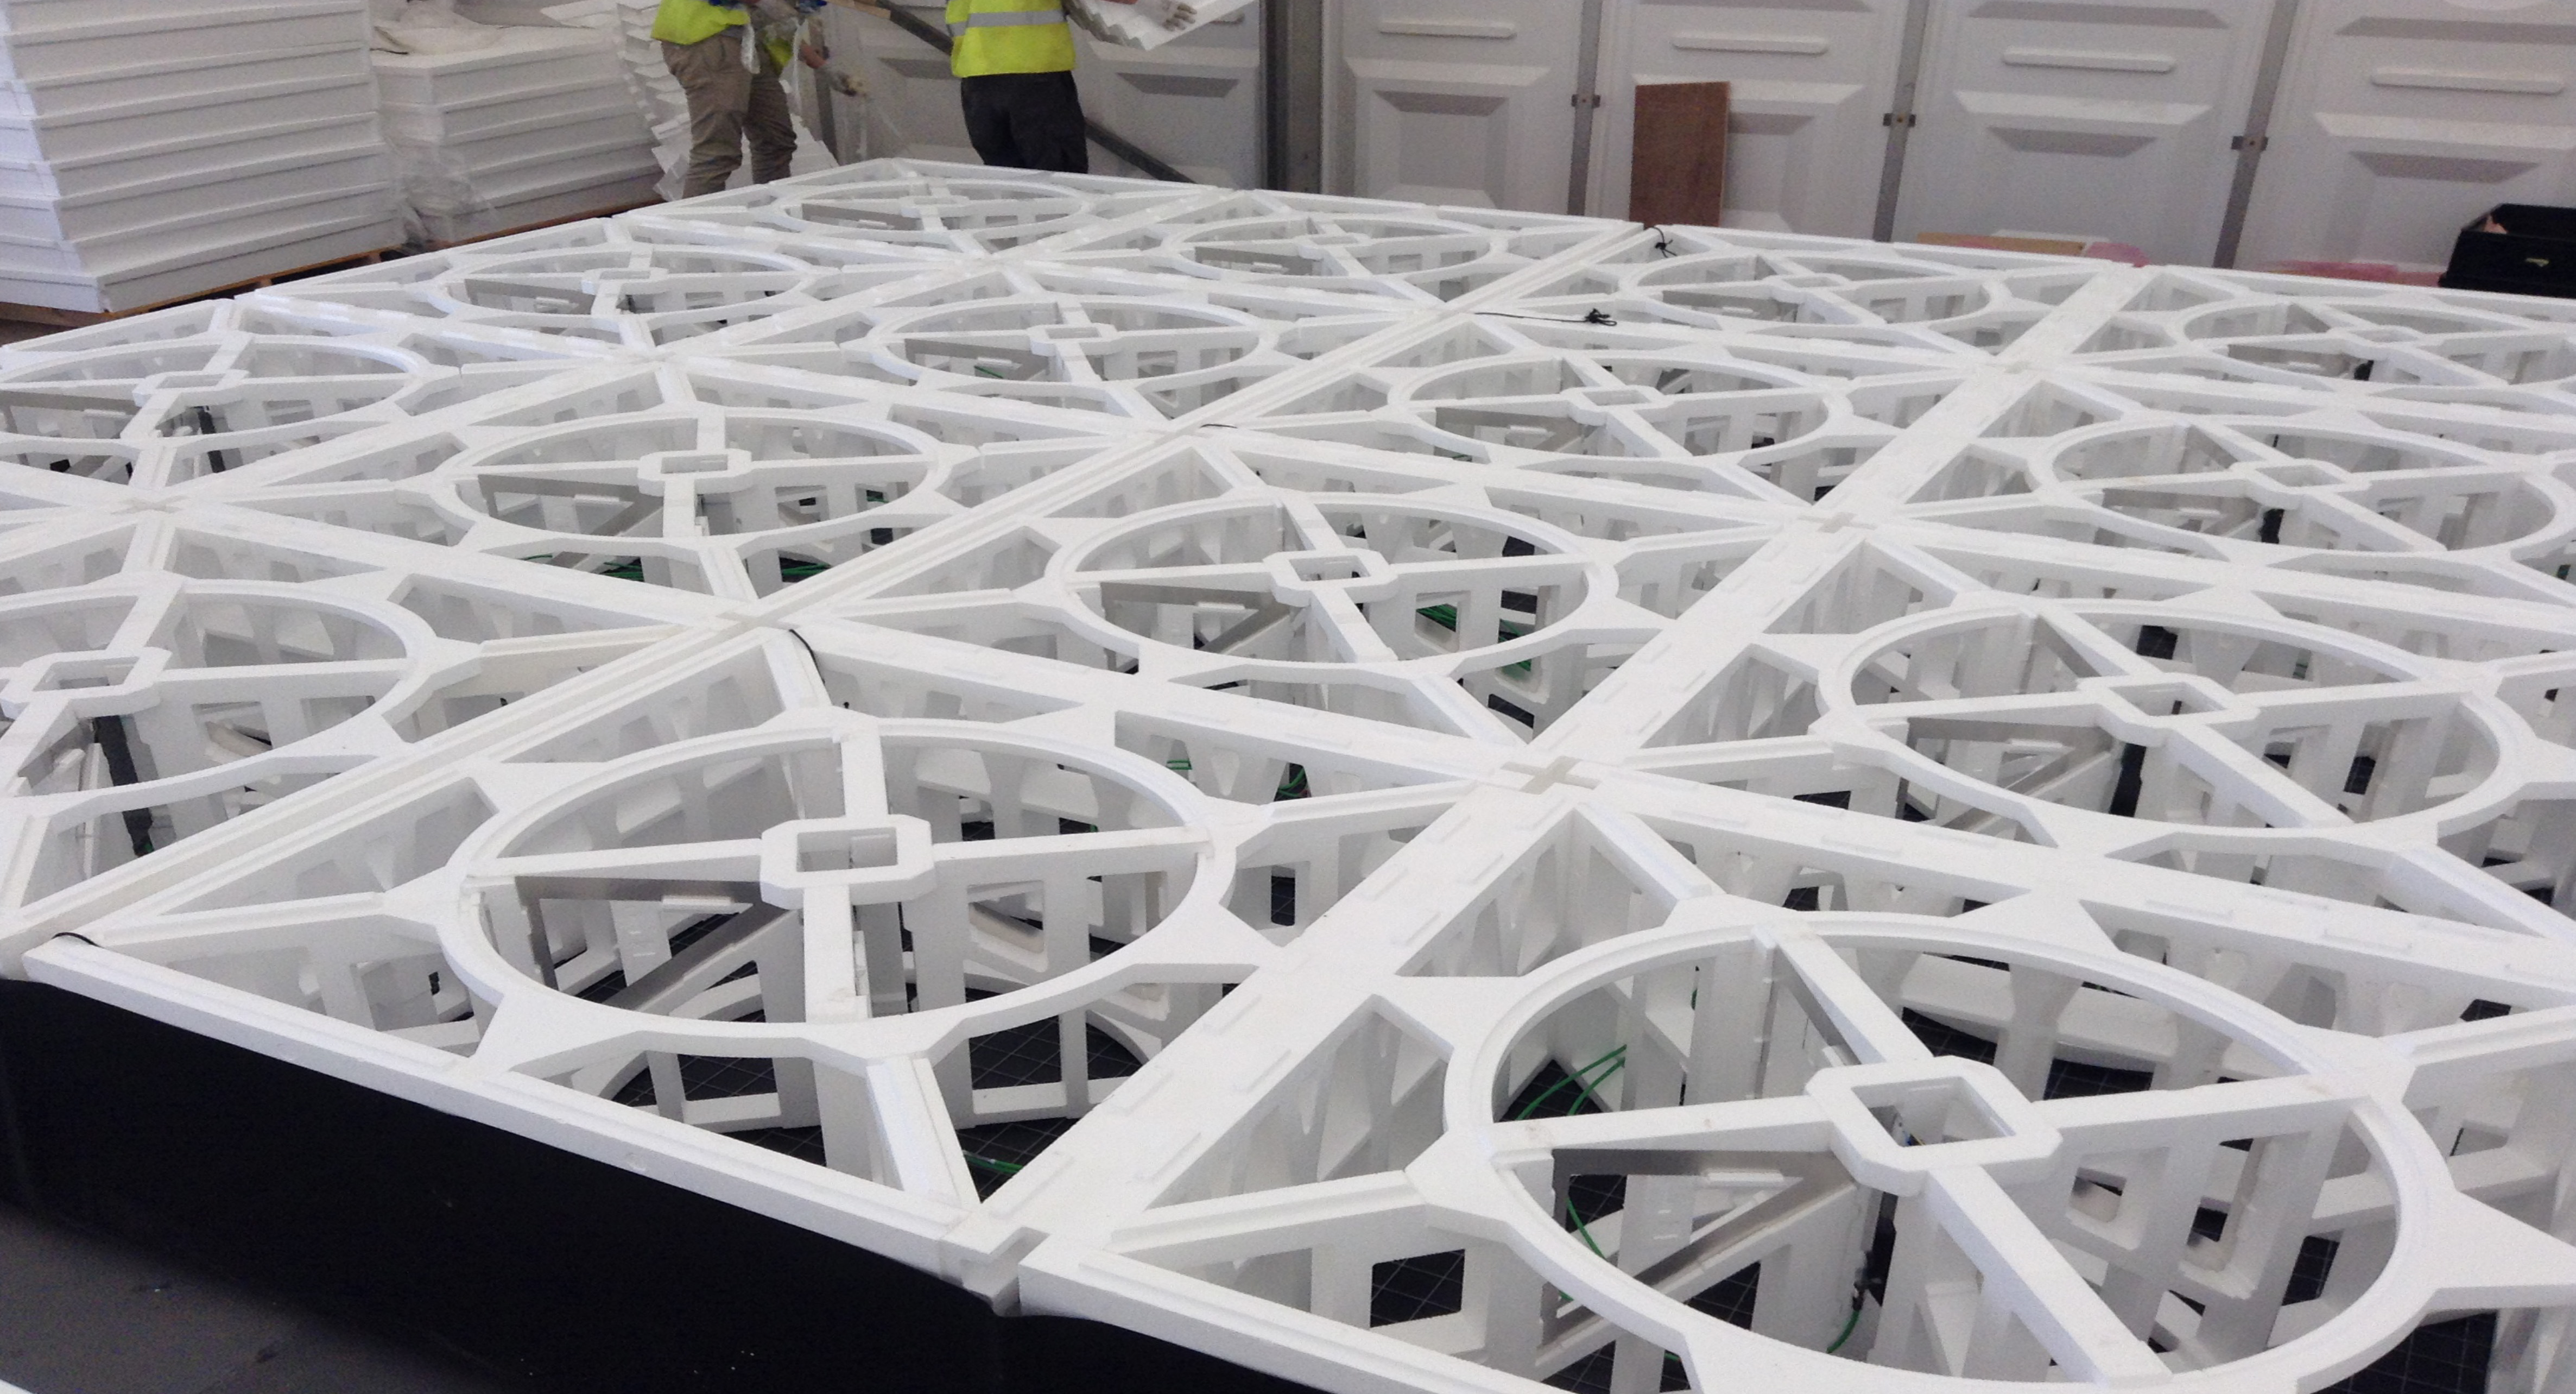
\includegraphics[width=\columnwidth]{HBA.jpg}
\caption[The inside of a High Band Antenna tile.]{A High Band Antenna before the tile lid has been placed. The  4 $\times$ 4 grid of bow-tie cross dipole antenna elements is clearly visible inside the expanded polystyrene casing.}
\label{fig:HBA}
\end{figure}

Each antenna element in a HBA tile is connected to a front-end which performs preamplification and analogue beamforming. Each front-end is then connected to a summator (one for each polarisation) where the signals from all antenna elements are summed before being sent for further signal processing in the station container, see section \ref{sec:sig_pipe}. The effect of analogue beamforming means that HBA observations are only sensitive to particular directions on the sky. Further to this, the regular gridding of the antenna elements leads to diffraction effects which makes all sky imaging with HBAs a less common observation type. The diffraction effects can be minimised by randomly excluding antenna elements however the reduces the sensitivity of such observations.

\begin{figure}[ht]
    \centering
    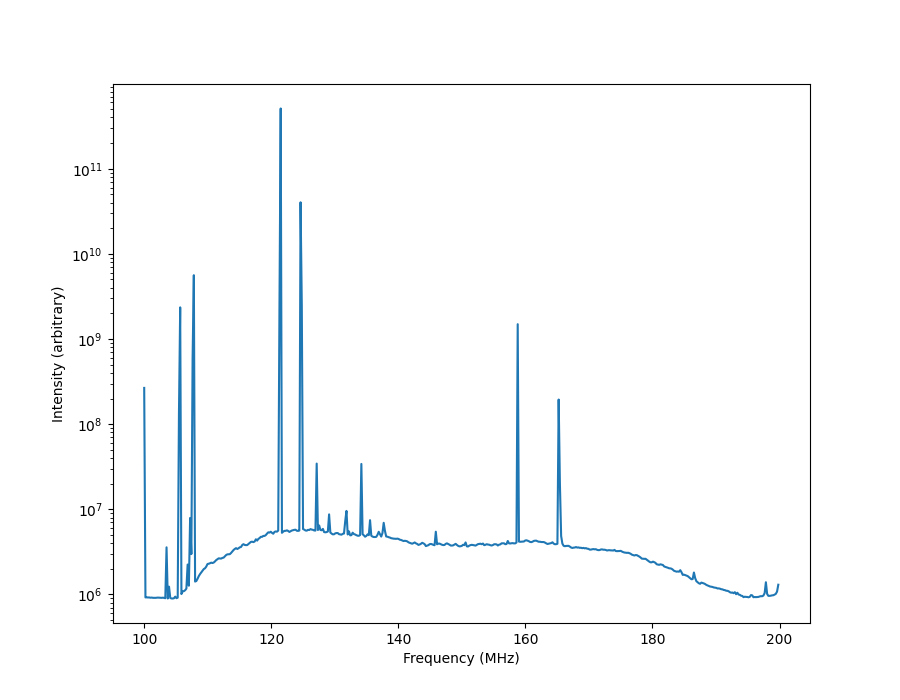
\includegraphics[width=\columnwidth]{hba_powerspec.png}
    \caption[Typical power spectrum for a HBA 100 - 200 MHz.]{Typical power spectrum for a HBA in the frequency range 100 - 200 MHz. Large peaks here are typically associated with noise from digital audio broadcasting (DAB) radio and other sources of RFI.}
    \label{fig:HBA_power_spec}
\end{figure}

\subsection{Remote Station Processing Boards (RSPs)}
\label{sec:rsp}
The Remote Station Processing boards (RSPs) perform the bulk of digital signal processing in a LOFAR station. Each LOFAR station consists of 24 RSP boards capable of channelising, beamforming and correlating raw voltage data recorded by either the LBAs or HBAs. A polyphase filter converts recorded data into 1024 complex subband signal which, because the signal is real, is fully described by the positive 512 subbands. These 512 subbands offer $\sim 195$kHz frequency resolution across the band. In order to perform beamforming, each RSP is connected together in a ring. Data is passed along this ring and summed in each RSP where a phase correction is also applied in order to ``point" the telescope beam. A maximum of 488 subbands can be used to create beamlets, beams pointed in a particular direction observing in a particular frequency. Data from this process is streamed to an external storage node from 4 points in the ring (i.e. from 4 RSPs) each containing one quarter of the beamlets computed by the RSP boards. Figure \ref{fig:RSP} shows a single RSP board from I-LOFAR.

\begin{figure}[ht]
\centering
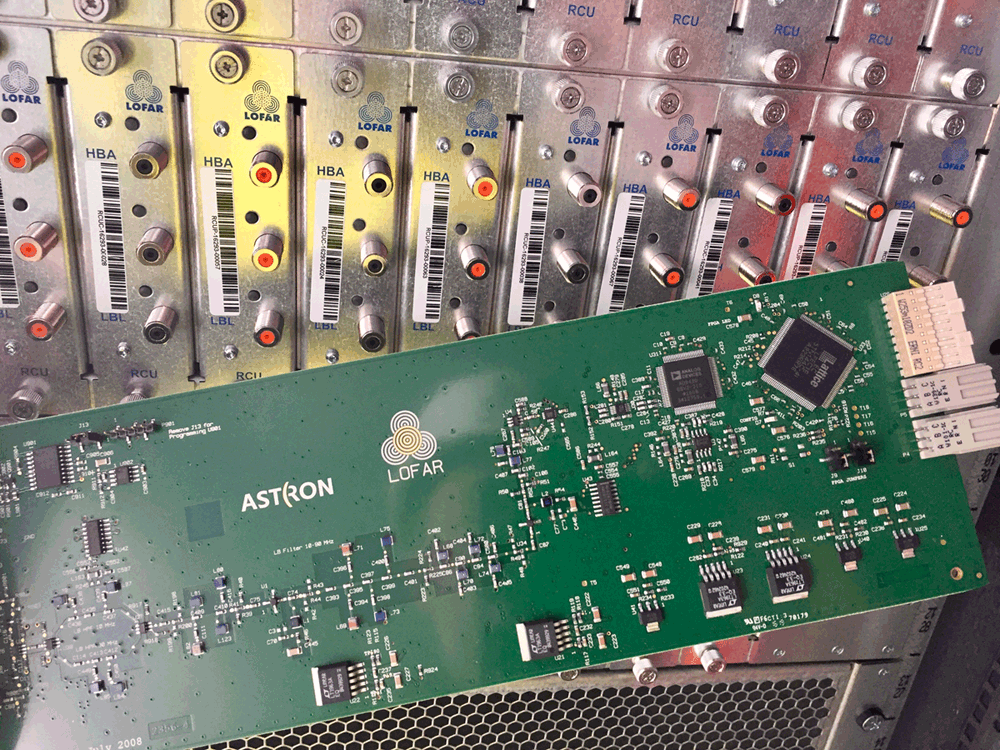
\includegraphics[width=\columnwidth]{RSP.png}
\caption[A Remote Station Processing board.]{A Remote Station Processing board from I-LOFAR.}
\label{fig:RSP}
\end{figure}

%Access to the data from RSP boards directly is possible provided there is a sufficient computer back end and network setup capable of writing the data being sent at 3.3Gbps.
\subsection{Transient Buffer Boards (TBBs)}
\label{sec:tbb}
One of the lesser used pieces of LOFAR hardware are the Transient Buffer Boards (TBBs). TBBs are RAM buffers that can temporarily store data at it's natively sampled 5ns time resolution. Each LOFAR station contains a total of 12 TBBs ranging from 1 GB to 32GB of memory. More recently completed stations such as I-LOFAR have 32GB TBBs while the older Dutch stations usually have less than 16GB.
%A single TBB stores data from 8 different antennas with 2 polaristions each  
A 32GB TBB can store up to 5 seconds worth of data recorded by a LOFAR station although this can be increased if fewer inputs or polarisations are recorded. TBBs are currently used in analysing cosmic ray showers \citep{Mulrey2020} and lightning storms \citep{Hare2018} but have yet to become a mainstream tool for solar physics, despite their potential. 
Recording the radio Sun at 5ns has never been attempted before and as such could offer a wealth of never before studied phenomena or cast new light onto long standing questions.
While the next generation telescopes like the Square Kilometre Array (SKA) and the Murchison Widefield Array (MWA) sample at higher rates than 5ns, none of them store full time resolution data. This gives LOFAR the unprecidented abiltiy to capture transient events at the highest temporal resolution ever. Figure \ref{fig:TBB} shows a single TBB.

\begin{figure}[ht]
\centering
\includegraphics[width=\columnwidth]{TBB_big.png}
\caption[A Transient Buffer Board.]{A Transient Buffer Board.}
\label{fig:TBB}
\end{figure}

\section{I-LOFAR: The Irish LOw Frequency ARray}
\label{sec:I-LOFAR}
Construction of the Irish LOFAR station (I-LOFAR) was completed in July 2017 on the demesne of Birr Castle, County Offaly, in the Irish Midlands. An international LOFAR station such as I-LOFAR consists of $96$ dual-polarisation dipole antennas known as Low Band Antennas (LBAs) which record radio frequencies of \SIrange{10}{90}{\mega\hertz} and $96$ High Band Antenna (HBA) tiles which each contain $16$ bow-tie antennas connected to an analogue summator and record in the frequency range \SIrange{110}{250}{\mega\hertz} \citep[see][ for a full description of LOFAR antennas]{VanHaarlem2013}. Data recorded by the antennas are then channelised into $512$ subbands of \SI{195.3125}{\kilo\hertz} (\SI{156.25}{\kilo\hertz}) frequency resolution at \SI{5.12}{\micro\second} (\SI{6.4}{\micro\second}) temporal resolution depending on the clock rate used to sample data, either \SI{200}{\mega \hertz} or \SI{160}{\mega \hertz} \citep{VanHaarlem2013}. The signal from each antenna is then digitally beamformed (BF) to a direction on the sky to create beamlets. A beamlet is a specific location on the sky observed at a specific subband. An international LOFAR station can record and process data in either 8 bits or 16 bits, corresponding to a maximum of 488 or 244 beamlets respectively. The term to describe how many bits are used during an observation is the bitmode. It is also possible to record and process at 4 bits. Beamlets are recorded at $3.2$~Gbps. When I-LOFAR is in local mode, the BF data is sent along a fibre connection to a local control room. Figure \ref{fig:ILOFAR} shows an aerial photograph of I-LOFAR. 

The total available bandwidth for I-LOFAR (and other international LOFAR stations) observations is determined by the bitmode used. This corresponds to a bandwidth of $\sim 47 \ (95, 190)$~MHz for 16 (8, 4) bit data. However, it is not necessary that the frequencies of each beamlet be sequential, which allows  a wider range of frequencies to be achieved. 
This is utilised in `mode 357', developed at the Kilpisjärvi Atmospheric Imaging Receiver Array \citep[KAIRA;][]{McKay-Bukowski2015}. In mode 357, beamlets are formed such that 200 beamlets from \SIrange{10}{90}{\mega\hertz}, 200 beamlets from \SIrange{110}{190}{\mega\hertz} and 88 beamlets from \SIrange{210}{240}{\mega\hertz} are recorded. In order to achieve this recording scheme, the number of antennas used for each frequency range is reduced. This leads to a lower sensitivity in mode 357. Mode 357 is particularly useful for observations of solar radio bursts, which typically occur across the entire LOFAR spectrum.

I-LOFAR produces a number of one second temporal resolution statistics files which are stored locally on the station's Local Control Unit (LCU). These are sub-band statistics (SSTs), which give the power spectrum for each antenna, beamlet statistics (BSTs), which give the power in each beamlet formed by the LOFAR station, and crosslet statistics (XSTs), the correlation coefficients between each antenna. These low-resolution data can be employed for system monitoring but are also sufficient for some astrophysical applications, for example, the XST data can be used to create snapshot all-sky images, and BST data have been used to study solar radio bursts \citep{Maguire2020}. The desire to use the full capabilities of the station, by accessing the full resolution is the motivation to develop a computational backend for the capture,  processing, and storage, of stand-alone BF data. 


\begin{figure*}[ht]
    \centering
    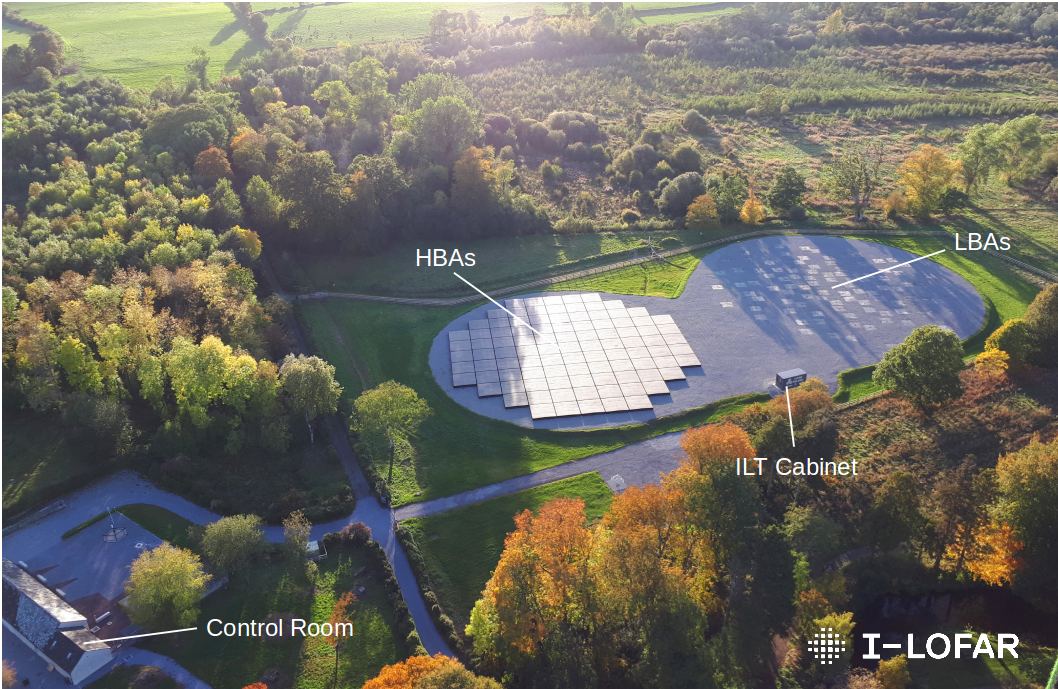
\includegraphics[width=\columnwidth]{I_LOFAR_balloon_labeled.png}
    \caption[Aerial photograph of the Irish Low Frequency Array station IE613 (I-LOFAR) at Birr Castle, County Offaly.]{Aerial photograph of the Irish Low Frequency Array station IE613 (I-LOFAR) at Birr Castle, County Offaly. Data from the LBAs and HBAs are transferred to the ILT Cabinet (centre right) via coaxial cables where they are amplified, filtered and digitised. In international mode, data are transported to Groningen in the Netherlands at $\sim$3.2~Gbps. In local mode, data are processed using REALTA in the I-LOFAR Control Room (bottom left). Image credit: Alison Delaney (Birr Castle).}
    \label{fig:ILOFAR}
\end{figure*}


One of the many benefits to using LOFAR as a radio telescope is that each station can be used independently in Single Station Mode which, in the case of international stations, gives freedom to the host countries to make specific observations that may not be covered in a LOFAR observing cycle. Not only this but Single Station mode offers the flexibility of the raw complex voltage data before it has passed through any averaging or calibration pipelines that occur during international observing mode.

This allows direct access to raw voltage data meaning any form of data processing imaginable can be performed. The only limit to this is the computer power and data storage available, two extremely non-trivial problems with LOFAR data. Recording complex raw voltage data from the RSPs requires a 10Gbps fibre optic link between the LOFAR cabinet and a powerful computer cluster. Due to the unpredictable nature of solar radio bursts, the only way to guarantee they will be recorded is to observe for many hours. Data quickly become terabytes in size which becomes challenging to perform any amount of post-analysis.
Another disadvantage of using Single Station mode is that, because the main appeal of LOFAR are its long baseline capabilities, little has been developed for Single Station use which only has a maximum baseline of $\sim 300$m however, for spectral work this is less of an issue.


\subsection{Digital Signal Processing for a Single LOFAR Station}
\label{sec:sig_pipe}
The LOFAR digital signal processing pipeline for a single station is outlined in Figure \ref{fig:sig_pipe}. Analogue signal is received by the HBAs or LBAs. This is sampled at 200,000,000 samples per second and converted to a digital signal by a 12 bit A/D converter inside the station's Receiver Units (RCUs). Each RCU digitises data for 1 antenna feed (X or Y polarisation) so there are $96 \times 2 = 192$ RCUs in total. The digitised data is then sent to the RSP boards. In a standard LOFAR observation while the station is in International LOFAR Telescope (ILT) mode, data from 8 RCUs are channelised into 512 subbands by a polyphase filter bank. This results in raw complex voltage data at 195.3125kHz frequency resolution and 5.12$\mu$s temporal resolution which are then phase shifted and added together in order to beamform to a particular location on the sky (see \ref{sec:beamform_theory}). The output from each of the 24 RSP boards are added in a ring before being sent along a 10Gbps fibre link to Groningen and passed into the COBALT2.0 processing cluster where the data can be further channelised and correlated to produce interferometric or beamformed data products.
The digital signal processing pipeline is much the same in Single Station Mode however, data is averaged out to 1 second before being saved as various ``statistics" files. These include subband statistics, which give the power spectrum for each antenna; beamlet statistics, give the power in each beamlet formed by the LOFAR station; and crosslet statistics, the correlation coefficients between each antenna which can be used to create all sky images.
Parallel to this, the raw voltage signal with the full 5ns temporal resolution is stored in the memory of a TBB. A single LOFAR station has 12 TBBs which take 2 RSP boards as inputs each. The buffer will constantly overwrite itself until it is frozen and dumped either by an internal/external trigger signal or sending a dump command manually.

\begin{figure}[ht]
    \centering
    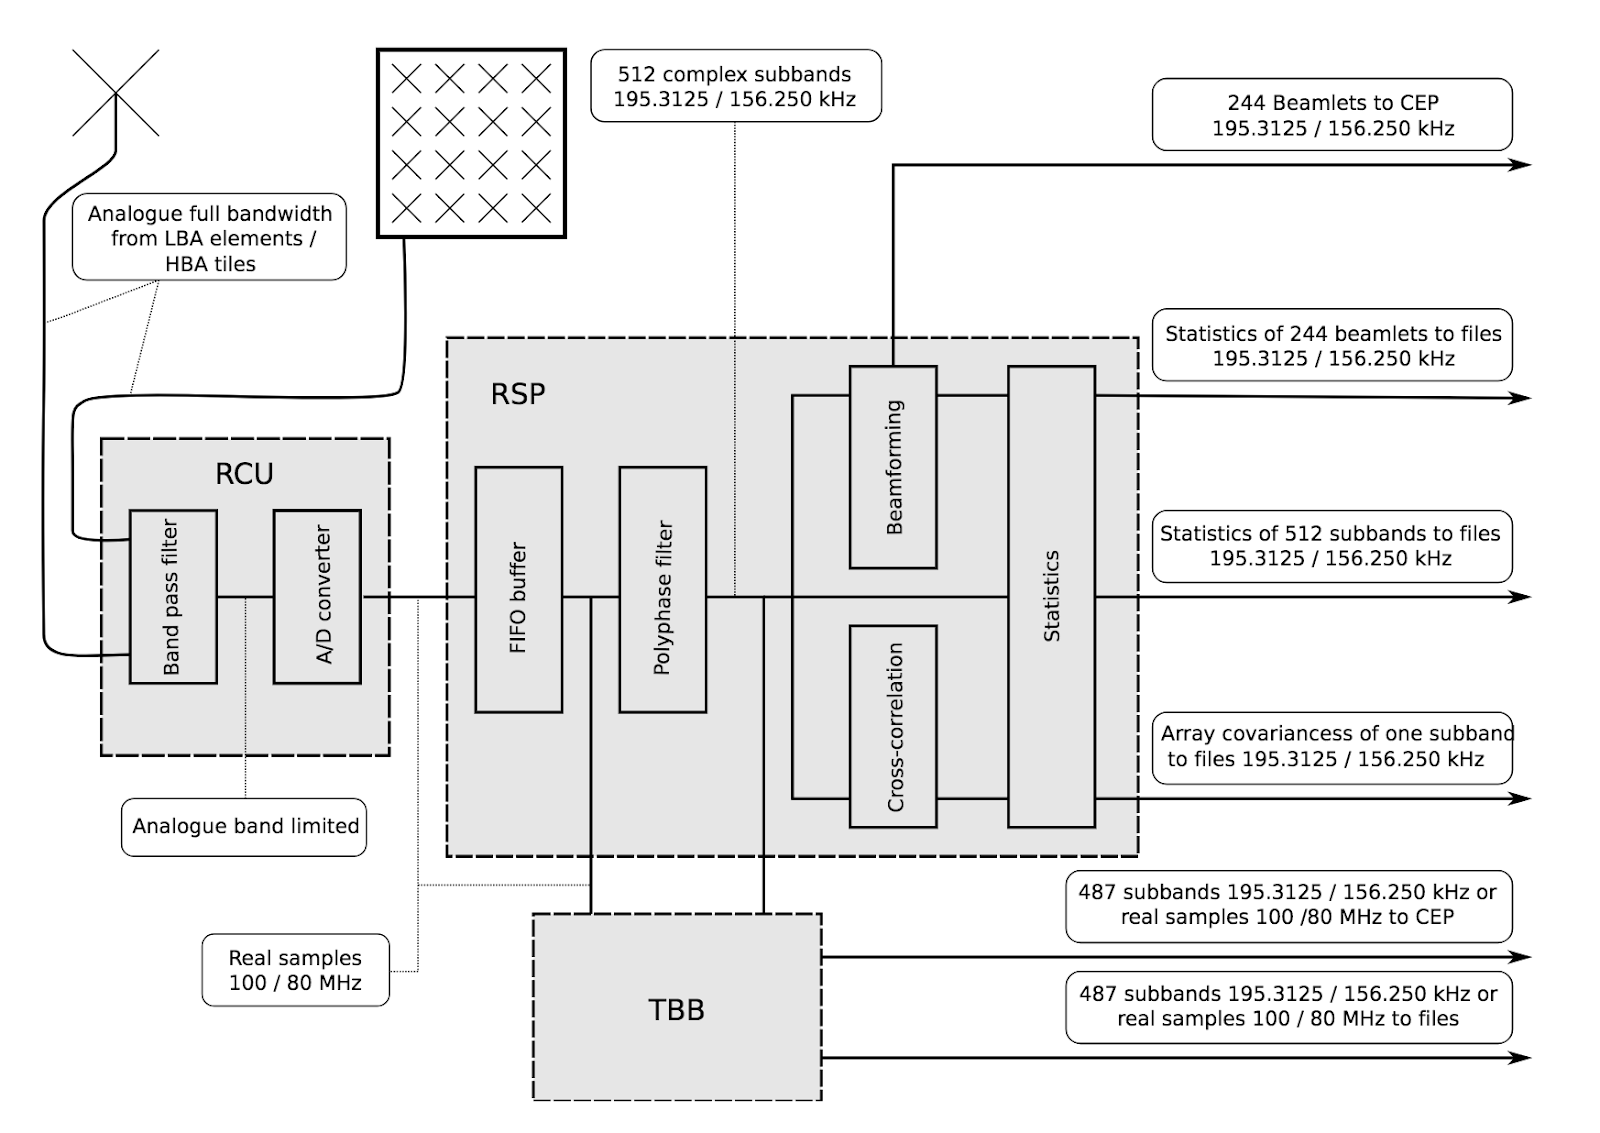
\includegraphics[width=0.75\columnwidth]{Images/Digital_signal_processing.png}
    \caption[Digital signal processing pipeline of an individual LOFAR station.]{Digital signal processing pipeline of an individual LOFAR station. Data is first digitised in the ReCiever Unit (RCU) before being sent to the RSP board. Here data is channelised by a polyphase filter and beamformed before being sent to the CEntral Processor (CEP) in the Netherlands. Also featured is the TBB which stores data in a ring buffer unless it is read out to an external storage system. }
    \label{fig:sig_pipe}
\end{figure}

%\section{The REALtime Transient Acquisition Backend (REALTA)}
%Modern radio interferometers such as the LOFAR are capable of producing data at hundreds of gigabits to terabits per second. This high data rate makes the analysis of radio data cumbersome and computationally expensive. While high performance computing facilities exist for large national and international facilities, that may not be the case for instruments operated by a single institution or a small consortium. 
%Data rates for next generation radio telescopes are set to eclipse those currently in operation, hence local processing of data will become all the more important.
%Here, we introduce the REAL-time Transient Acquisition backend (REALTA), a computing backend at the Irish LOFAR station (I-LOFAR) which facilitates the recording of data in near real-time and post-processing. We also present first searches and scientific results of a number of radio phenomena observed by I-LOFAR and REALTA, including pulsars, fast radio bursts (FRBs), rotating radio transients (RRATs), the search for extraterrestrial intelligence (SETI), Jupiter, and the Sun.
%
%\subsection{Introduction}
%\label{sec:realta_intro}
%Modern radio interferometers produce more data than any astronomical instrument in history. Interferometric observations can receive data at hundreds of gigabits per second, requiring high performance computer (HPC) facilities to preprocess data before it can be analysed and scientifically explored. With newly built telescopes such as the Murchison Widefield Array \citep[MWA;][]{Lonsdale2009}, MeerKAT \citep{Jonas2016} and the Australian Square Kilometre Array Pathfinder \citep[ASKAP;][]{Johnston2008} acquiring such vast amounts of data \citep[up to $300$~Gbps;][]{Voronkov2020, Lonsdale2009} radio astronomy is working at the cutting edges of big data science. The Square Kilometre Array \citep{McMullin2020} is commencing construction this year and pushes the computational requirements to ever more difficult regimes \citep{Scaife2020}.
%
% The detailed differences between the station types are described in \cite{VanHaarlem2013}, one key difference being that international stations have twice the collecting area of a Dutch core or remote station. LOFAR operates in two modes: international mode, also known as International LOFAR Telescope (ILT) mode, and local, or stand-alone, mode. In ILT mode, data from all the LOFAR stations in the network are sent via fibre optics to the COBALT2.0 correlator \citep[an upgrade to COBALT1.0,][]{Broekema2018} in Groningen, in the Netherlands. In local mode, each international station is operated by the host institute or consortium. \textit{De novo}, international stations do not have dedicated processing backends. Without such an addition the raw data from an international station could not be recorded or analysed. 
%
%The REAL-time Transient Acquisition backend (REALTA; from the Irish word for star, \textit{r\'ealta}) is a seven node computer cluster designed to record and analyse the raw BF data from international LOFAR stations in real-time, implemented at I-LOFAR. It takes inspiration from the ARTEMIS backend at the LOFAR-UK station in Chilbolton \citep{Serylak2012,Karastergiou2015}, although it significantly improves upon its hardware composition, using modern components with greater computational power. The REALTA hardware is available commercially, and as such REALTA can be implemented at any international LOFAR station and is ideal as a generic computing backend for LOFAR local mode observations.
%
%Telescope backends at other international LOFAR stations have been used to search for fast radio bursts (FRBs) and studying pulsars using LOFAR-UK \citep[for example,][]{Karastergiou2015}, the French LOFAR station at Nançay \citep[for example,][]{Rajwade2016,Bondonneau2017}, and its extension, NenuFAR \citep[for example,][]{Bondonneau2020}, the German stations \citep[e.g][]{Donner2019, Porayko2019, Tiburzi2019}, and the combination of a number of international stations \citep[for example,][]{Mereghetti2016, Hermsen2018, Michilli2018}. Here we showcase similar success in these and various other observations using I-LOFAR and REALTA. 
%
%% Telescope backends at other international LOFAR stations have been used to search for fast radio bursts (FRBs) and studying pulsars using LOFAR-UK, \textbf{the French LOFAR station at Nançay and its extension, NenuFAR, the German international stations and the combination of a number of international stations \citep[for example,][]{Karastergiou2015, Rajwade2016, Bondonneau2017, Bondonneau2020b, Donner2019, Porayko2019, Tiburzi2019, Mereghetti2016, Hermsen2018, Michilli2018}.} Here where we showcase similar success in these and various other observations using I-LOFAR and REALTA. 
%
%The hardware for REALTA is further described in section~\ref{sec:REALTA} along with the networking configuration for the I-LOFAR control room while section~\ref{sec:softwareAndProcessing} describes the data capture and processing software used by REALTA. In section~\ref{sec:results}, some first scientific results from REALTA are highlighted. These include observations of pulsars, solar radio bursts, FRBs, Jovian radio emission, and the search for extraterrestrial intelligence (SETI).  %\textbf{Although data capture occurs in real-time, REALTA performs post-processing to data after it has been recorded. Development to bring the system ``online" is ongoing and this work is further outlined in section \ref{sec:future_work}.} %We conclude in section~\ref{sec:future_work} with a discussion on future work and the outlook for REALTA in the context of upcoming upgrades to LOFAR.
%
%\subsection{REALTA}
%\label{sec:REALTA}
%In this section, we describe the local network configuration necessary to capture raw User Datagram Protocol \citep[UDP;][]{Postel} packets from I-LOFAR and the individual hardware components that make up REALTA. Data is transferred from the station through the UDP protocol using LOFAR CEntral Processing (CEP) packets. Each packet is 7824 bytes long and consits of a 16 bit header followed by 16 time slices for each beamlet. The full specification for CEP packets is described in both \cite{Lubberhuizen2009} and \citet{Virtanen2018}.  CEP packets are sent via fibre optics to CEP or REALTA over four data `lanes'. Each lane only holds one quarter of the maximum number of beamlets for an observation.
%The network to facilitate capturing these packets is shown as a schematic block diagram in Figure \ref{fig:block}, while Table \ref{table:REALTAspecs} gives a detailed description of the specifications for each of the REALTA nodes. 
%
%\subsubsection{Local networking}
%\label{sec:network}
%The control room for I-LOFAR is located at the Rosse Observatory on the grounds of Birr Castle and $\sim$~100~m from I-LOFAR (Figure \ref{fig:ILOFAR}). In order to record data from I-LOFAR while it is in local mode, a high-speed $10$~Gbps network was set up between the ILT container that houses the I-LOFAR Remote Station Processing (RSP) boards and the control room.
%
%In a typical ILT observation, data output from each RSP board is sent to a Foundry LS648 10~Gbps network access switch (S2) in the container. From here it is sent to a Foundry LS624 switch (S1) before finally being sent over a 10~Gbps fibre connection to the COBALT cluster in Groningen for correlation and or beamforming with data from other LOFAR stations.
%
%The aim of I-LOFAR's network configuration is to record RSP data to REALTA in the I-LOFAR control room. This is achieved by a fibre link between the I-LOFAR control room and S1. RSP data are sent along a Virtual Local Area Network (VLAN), VLAN 2278, on a 10~Gbps fibre link to the control room. Data reaches a fibre optic termination panel in the I-LOFAR control room and is sent to a 10~Gbps Dell EMC S4128F-ON optical switch. A fibre link between this switch and the REALTA compute nodes allows data to be recorded. All REALTA compute nodes are connected via Infiniband (an alternative to Ethernet and fibre). On REALTA this acts at a maximum of 10~Gbps to allow for transfer of data between nodes and Network File System (NFS) mounting.
%
%As well as this, a future link to a HEAnet (Ireland’s national education and research network) cloud service for data transfer to the research institutions of the I-LOFAR consortium has been approved by ASTRON. This will allow access along existing 10~Gbps fibre infrastructure to S1 and then over another fibre to the control room along a VLAN. Another fibre is in place to eventually send RSP and Transient Buffer Board (TBB) data directly from S2 to the control room using two additional VLANs.
%Data transfer from REALTA to research institutes is currently facilitated by a direct 1~Gbps between the Dublin Institute of Advanced Studies (DIAS) and S1 via HEAnet on a VLAN.
%
%\subsubsection{Hardware description}
%REALTA is ultimately designed to perform real-time analysis of radio data generated by the I-LOFAR international station. In its current form, it uses four Dell Poweredge R740XD compute nodes named UCC1, UCC2, UCC3, and UCC4. Each compute node contains two Intel Xeon\textsuperscript{\textregistered} Gold 6130 central processing units (CPUs) and an NVIDIA Tesla V100 16GB graphics processing unit (GPU). Each CPU has 16 cores, with two threads per core giving a total of 64 threads per node.  A total of $210$~TB of storage is distributed across the compute nodes with a further $128$~TB available on a dedicated storage server, NUIG1. Storage on REALTA is set up as a Redundant Array of Inexpensive Disks (RAID). Most disks ($\sim 263$~TB) are in RAID 5 for data archival, while a number of scratch disks ($\sim 75$~TB) are set up in RAID 0 for recording and processing raw data. In addition to this, a compute node for dedicated SETI research was provided by the Breakthrough Prize Foundation in collaboration with the Breakthrough Listen (BL) team at the Berkeley SETI Research Centre. The BL compute node is a SuperMicro 6049P-E1CR24H node with two, 16 core (8 threads) Intel Xeon\textsuperscript{\textregistered} Silver 4110 CPUs, an NVIDIA RTX 2080Ti GPU, and $144$~TB of storage. The BL Headnode is a SuperMicro 1029U-TRTP2 node intended to control REALTA during SETI observations. When being operated from the BL Headnode, all of the REALTA compute nodes will receive an identical operating system (OS) image and process in parallel across all five compute nodes. Each of the REALTA nodes connect to the 10~Gbps Dell EMC S4128F-ON optical switch via fibre optic cable as well as a 1~Gbps Ethernet switch for normal networking (using default VLAN 1). There are two redundant keyboard-video-mouse (KVM) servers and a KVM switch for remote access to both switches and all machines, and three uninterruptible power supplies (UPS) to mitigate the effects of a sudden power outage on both servers and critical access paths. Fail-safe cold-aisle air-conditioning will handle heat created by this unsupervised cluster.
%
%\begin{figure*}[h]
%    \centering
%    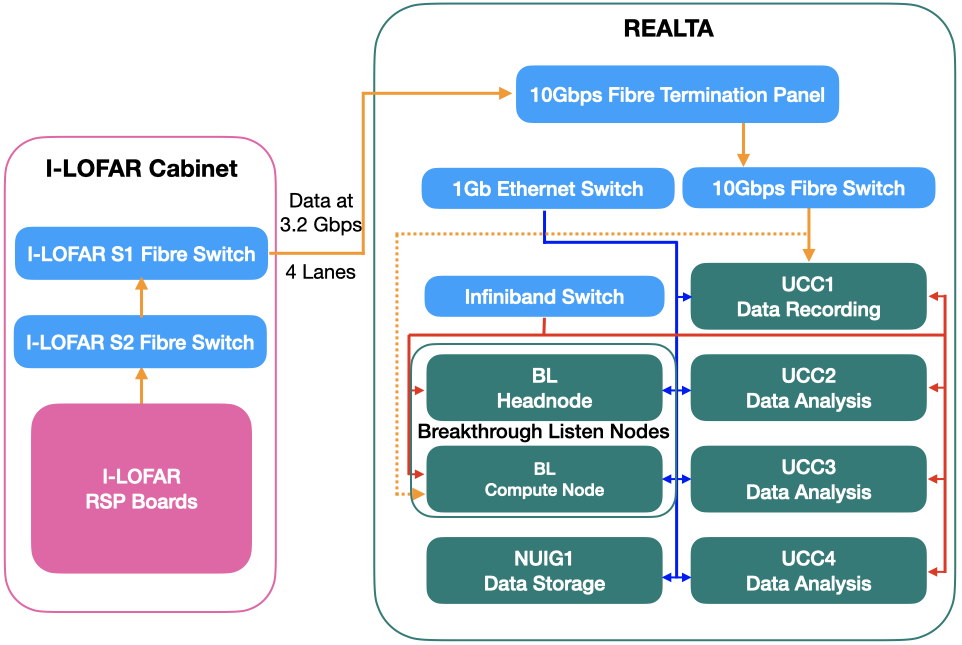
\includegraphics[width=0.7\linewidth]{REALTA_block_ref.png}
%    \caption[Block diagram for REALTA and I-LOFAR.]{Block diagram for REALTA and I-LOFAR. Data recorded at the Remote Station Processing (RSP) boards are sent to the S1 fibre switch in the I-LOFAR container. Here the data are split into four `lanes' where each lane contains the data from a maximum of one quarter of the beamlets from the observation. The four lanes of data are then sent over a fibre connection to the I-LOFAR control room where it is recorded by REALTA. Orange arrows indicate the data path along fibre connections. Blue arrows are 1~Gbps Ethernet links and red arrows show infiniband connectivity. The dotted orange line is a fibre link to the BL compute node currently under development.}
%    \label{fig:block}
%\end{figure*}
%
%REALTA is located in the control room which is $\sim 100$~m from the I-LOFAR HBAs and $\sim 150$~m from the LBAs. As REALTA was being set up and tested, the RFI from the system was monitored using all-sky observations and sub-band statistics observations. It was found that REALTA did not produce any significant RFI.
%
%Table \ref{table:REALTAspecs} lists the technical specifications for each of the nodes in REALTA. In its configuration at the time of writing, REALTA acts as a number of independent nodes (UCC1-4, NUIG1, BL headnode, and BL Compute node). Data is recorded solely to the UCC1 compute node while the remaining nodes perform pre-processing and data analysis after data has finished recording. 
%
%\begin{table*}\centering
%
%\begin{tabular}{l L{4.5cm} L{4.5cm}}
%
%  & Storage Node (NUIG1) & Compute Nodes ($\times 4$ UCC1-4 )  \\
% \hline
%Machine Model & Dell Poweredge R730XD & Dell Poweredge R740XD \\
%CPU  Model     & Intel Xeon\textsuperscript{\textregistered} E5-2640 V4 ($\times 2$)      &  Intel Xeon\textsuperscript{\textregistered} Gold 6130 ($\times 2$)       \\
%CPU Clock Speed & 2.40GHz & 2.10GHz \\
%CPU Cores (Threads) & 20 (40) & 32 (64)  \\
%RAM       & 256GB        & 256GB          \\
%Storage   & 128TB        & 210TB (total)          \\
%GPU &  N/A & 16GB NVIDIA Tesla V100 \\
% & & \\
%\end{tabular}
%
%%\bigskip removed because causing weird gaps in text
%\begin{tabular}{l L{4.5cm} L{4.5cm}}
%
% & BL Headnode & BL Compute Node   \\
% \hline
%Machine Model & SuperMicro 1029U-TRTP2 & SuperMicro 6049P-E1CR24H \\
%CPU  Model    &  Intel Xeon\textsuperscript{\textregistered} Silver 4110 ($\times 2$)        & Intel Xeon\textsuperscript{\textregistered} Silver 4110 ($\times 2$)\\
%CPU Clock Speed & 2.10GHz & 2.10GHz \\
%CPU Cores (Threads) & 16 (32) & 16 (32) \\
%RAM       & 93GB        & 96GB      \\
%Storage   &  N/A        & 144TB      \\
%GPU & N/A & 11GB NVIDIA RTX 2080Ti \\
%
%\end{tabular}
%
%%\bigskip removed because causing weird gaps in text
%\caption[Table of hardware specifications for REALTA.]{Table of hardware specifications for REALTA. Note that the specifications are given for individual UCC 1-4 compute nodes, except for storage which is the total amount dedicated to archival of data distributed across all four. }
%\label{table:REALTAspecs}
%\end{table*}
%
%\subsection{Software and pipelines}
%\label{sec:softwareAndProcessing}
%In REALTA's current state, UDP packets are recorded directly to disk before being converted into usable science products, such as Stokes parameters with variable levels of time integration, after the observation has completed. Future work will implement the current software pipelines to work directly on incoming data, which will allow for real-time analysis of the low frequency sky. Currently, a combination of local and community developed software is used in the main data recording and reduction pipeline. The primary recording and processing of the pipeline are described below.
%
%\subsubsection{Recording data}
%\label{sec:preproc}
%The station RSPs generate a stream of packets across four data lanes, which is recorded on our compute nodes using software developed by Olaf Wucknitz at the Max Planck Institute for Radio Astronomy. The recording software, \texttt{dump\_udp\_ow}, listens to each port for incoming CEP packets, discards the UDP metadata related to the protocol, and writes the remainder of the packets to disk.
%
%In order to reduce the storage requirements to record the CEP packets, the software can compress the data while it is being captured. This is accomplished by applying the \texttt{zstandard} compression algorithm\footnote{\hyperref[zstandard]{https://github.com/facebook/zstd}} to the output data stream. This procedure requires additional CPU processing but offers a compression fraction in the range of 40-60\%, depending on the observing mode and noise of an observation.
%
%\subsubsection{Pre-processing data}
%\label{sec:baseproc}%x
%% 3 main operations: reforming, detection, coherent dedispersion + detection
%% -- CLI extraction
%% -- ASCII / BL formatting / rawspec
%% -- CDMT extraction
%% -- CDMT stuff cut out from from Pulsar subsection, to be rewritten in new context
%Once the data has been recorded to disk, observers use \texttt{udpPacketManager}\footnote{\hyperref[udpPacketManager]{https://github.com/David-McKenna/udpPacketManager}} \citep{McKenna2020}, a C library developed to convert the raw CEP packets, either compressed or uncompressed, to usable scientific data products. It implements checks to correct for issues that may have occurred during the recording process, such as padding when packets are missed, performs a polarmetric correction on the voltages using \texttt{dreamBeam}\footnote{\hyperref[dreamBeam]{https://github.com/2baOrNot2ba/dreamBeam/}}, and generates scientific data products for further processing and analysis.
%
%The \texttt{udpPacketManager} library is extremely versatile and allows for an observer to chose a number of processing strategies. These include individual polarisation analysis, forming Stokes parameters, ordering data by either time or frequency or formatting data to be used with other software for further analysis. The most common processing strategy is to construct Stokes I and V from the voltages, then output the results to disk in a binary file format that follows the \texttt{SIGPROC} Filterbank standard \citep{Lorimer2011}. Future work will include determining best practises for removal of RFI from filterbank formatted files.
%
%% -- These next two subsections need better names.
%
%\subsubsection{Pulsar and single pulse processing}
%\label{sec:pulsarproc}
%% -- Pulsar Folding, DSPSR\citep{vanStraten2011}, PSRCHIVE\citep{Hotan2004}, PRESTO\citep{Ransom2001NewPulsars}
%
%% A typical pulsar observation is initially ingested from the station and saved to disk as raw voltages for further offline processing.  
%
%All pulse-like observations undergo an additional processing step, whereby data are both channelised by a factor of eight (reducing the bandwidth of a given observing subband to 24.41~kHz) and coherent dedispersion is applied to the voltages.
%%to increase the quality of the output data from the station. 
%Coherent dedispersion is the process by which an input signal is convolved with the inverse transfer function of the inter-stellar medium in order to remove the signature of dispersion delay due to free elections along the line of sight \citep{Hankins1987}. This process is especially important at frequencies observed by LOFAR as these delays scale with the inverse square of the observing frequency. This process is performed on the GPUs in REALTA using a modified version of \texttt{CDMT} \citep{Bassa2017}, which accepts input voltages from \texttt{udpPacketManager} rather than h5 files generated from the LOFAR COBALT system. In order to avoid distortions caused by Fast Fourier Transform (FFT) operations on zero-padded data, \texttt{CDMT} was further modified to overlap the input voltages between processing iterations.% and introduces overlapping of real data to suppress distortions in the output data from 0-padding the Fast Fourier Transform operations.
%
%Pulsar data is further reduced using a combination of \texttt{digifil} and \texttt{DSPSR} \citep{vanStraten2011} to generate folded profiles which are then analysed using \texttt{PSRCHIVE} \citep{Hotan2004}. The filterbanks are also often folded using \texttt{PRESTO} \citep{Ransom2001} to determine optimal dispersion measures for folding observations. RFI flagging is performed in two steps. Firstly, all data below 106~MHz and above 194~MHz is automatically flagged to remove contributions from local FM radio transmission and to minimise noise contributions due to the loss in sensitivity near the edge of the telescope's polyphase filter. Secondly, the spectral kurtosis method is performed by \texttt{DSPSR} during the folding step to remove transient RFI sources.
%
%Single-pulse sources, such as intermittent rotating radio transients \citep[RRATs;][]{McLaughlin2006} and fast radio bursts \citep[FRBs;][]{Lorimer2007,Thornton2013} are searched for using \texttt{Heimdall}\footnote{\hyperref[Heimdall]{https://sourceforge.net/projects/heimdall-astro/}} to generate pulse candidates across a wide dispersion measure range. A typical search is performed between 5~pc~cm$^{-3}$ and 500~pc~cm$^{-3}$ across all pulsar and single-source observations. These are then filtered, discarding any below the $7.5~\sigma$ level to reduce the number of spurious candidates due to system noise or alignment of RFI between frequency channels. The remaining candidates are then plotted and visually inspected to discard those that are due to RFI, ionospheric scintillation or other phenomena that may cause spurious signals. 
%
%% \label{proc:singlepulse}
%% \subsubsection{Single Pulse Detection}
%% -- Pulse Searching, Heimdall\footnote{https://sourceforge.net/projects/heimdall-astro/}
%
%% The generated data products normally take the form of a Stokes I \texttt{SIGPROC} filterbanks\citep{Lorimer2011\texttt{SIGPROC}:Programs}, which can then be used as the user sees fit. 
%%putting this here to have it at top of page 5
%
%\subsubsection{SETI data processing}
%\label{sect:pipeline_SETI}
%For SETI, the goal is to achieve a very high spectral resolution of the order of a few hertz to look for narrow-band Doppler drifting signals. Such signals are prime candidates for deliberately transmitted beacons by Extra-Terrestrial Intelligence \citep[ETI;][]{Tarter2001}. Baseband voltages are first recorded as described in section~\ref{sec:preproc} directly on the BL compute node. The \texttt{udpPacketManager} library is then used to convert these data to Green Bank Ultimate Pulsar Processing Instrument\footnote{\hyperref[GUPPI]{https://safe.nrao.edu/wiki/bin/view/CICADA/GUPPiUsersGuide}} (GUPPI) formatted baseband data products for further processing. The BL team has developed a suite of software to work with the GUPPI formatted baseband voltages \citep{Lebofsky2019} and the preliminary result from this software is discussed in section~\ref{sec:results}. 
%
%\subsubsection{Future development and real-time analysis}
%\label{sec:future_software}
%The current and planned data path through REALTA, from the time it is recorded at I-LOFAR to when it is written to disk by REALTA is shown as a block diagram in Figure \ref{fig:REALTA_future}. UDP packets containing the data are captured and recorded directly to disk in real-time (section \ref{sec:preproc}). The data are then formatted and metadata updated (\S \ref{sec:baseproc}) so that they are compatible with existing pulsar and SETI software (section \ref{sec:pulsarproc}, \ref{sect:pipeline_SETI}).
%
%In the future, the capture and formatting of data will occur simultaneously in real-time. Further channelisation of the raw data in the data capture stage will be implemented in order to increase the spectral resolution of observations and help in flagging Radio Frequency Interference (RFI) in the data. This, along with the generation of quick-look plots, will form the data preparation stage. The data processing software described below will also be developed to allow for real-time processing of solar, pulsar, FRB, RRAT, SETI, and other data. Finally, the data archive will be expanded to include a catalogue of transient events observed and a summary of their features.
%
%\begin{figure*}[t]
%    \centering
%    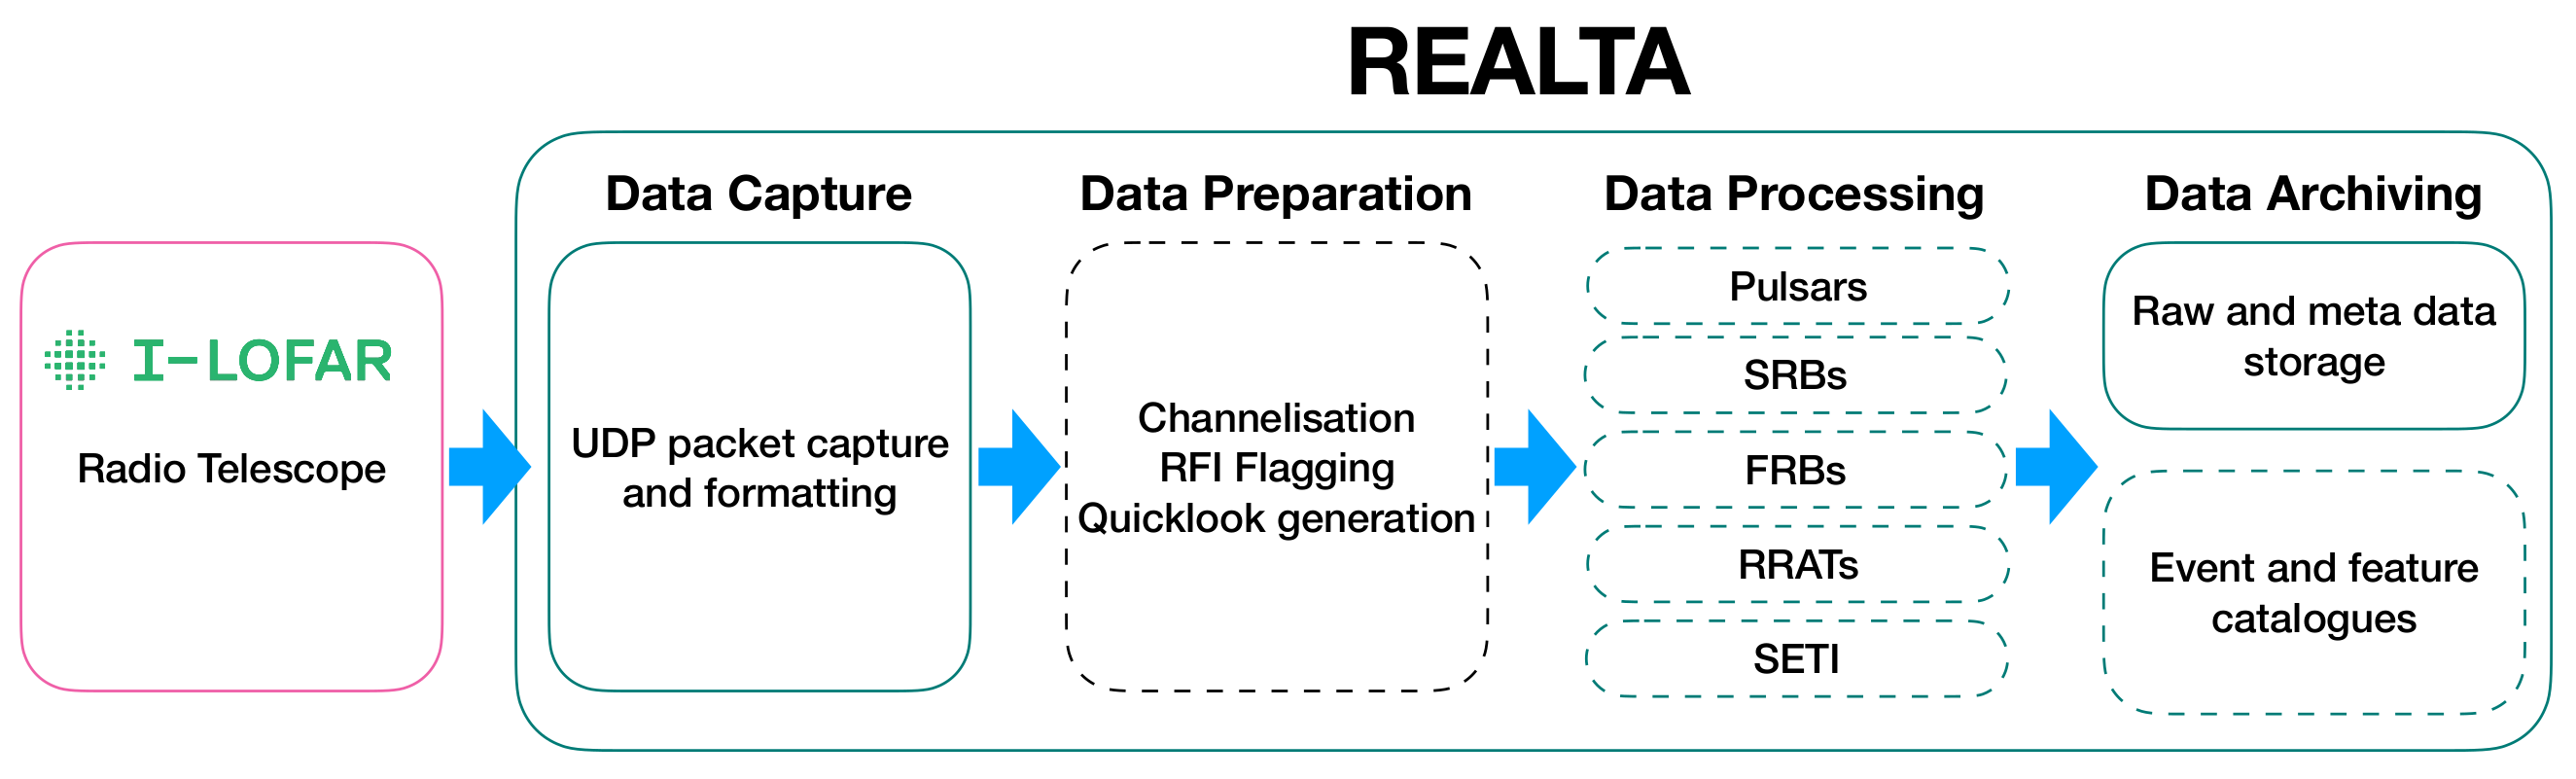
\includegraphics[width=0.75\linewidth]{REALTA_future_alt.png}
%    \caption[System diagram for REALTA.]{System diagram for REALTA, including future data preparation, processing, and archiving capabilities. Solid lines indicate existing features, while dashed lines denote stages under development. REALTA is currently capable of capturing data from the I-LOFAR radio telescope and archiving it in near real-time. We are in the process of developing a variety of data processing pipelines that will flag RFI, identify and characterise SRBs, pulsars, RRATs, FRBs, and SETI signals. Machine learning methods are being explored for a number of these tasks.}
%    \label{fig:REALTA_future}
%\end{figure*}
%
%%\begin{figure*}[t]
%%    \centering
%%    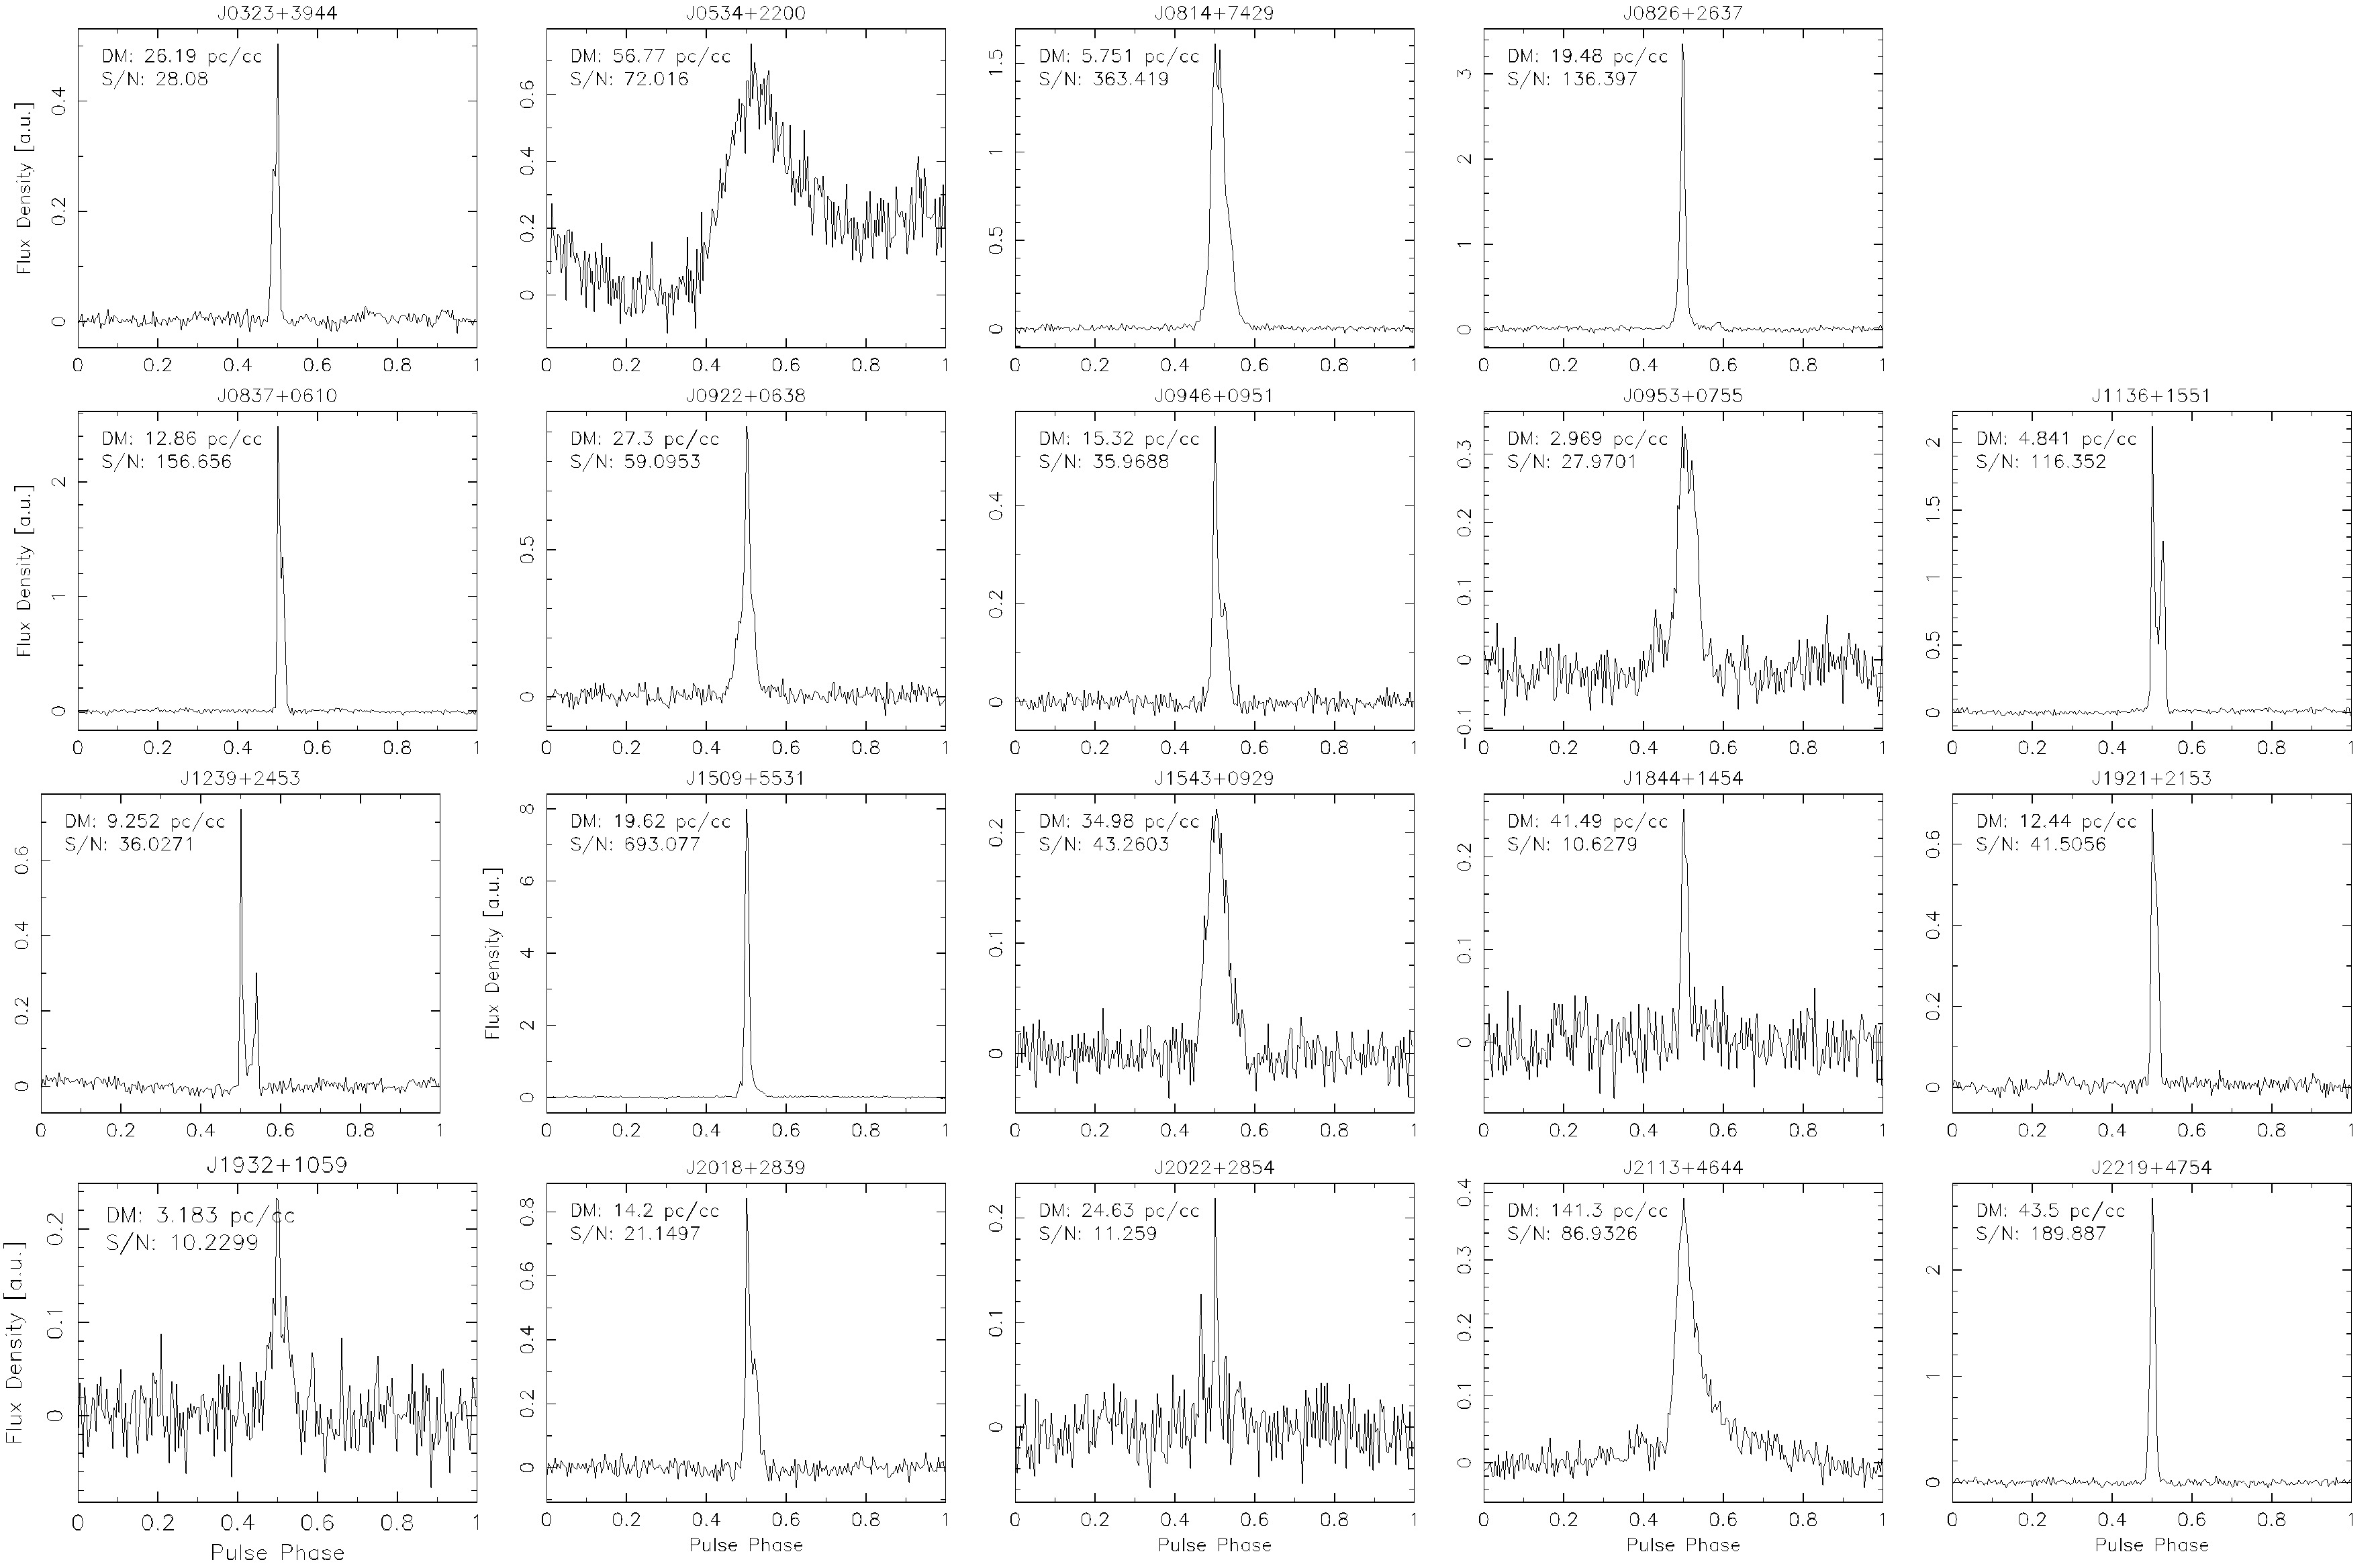
\includegraphics[width=0.92\textwidth]{psr_profiles.jpg}
%%    \caption[Sample of 19 pulsars observed with I-LOFAR and REALTA.]{Sample of 19 pulsars observed with I-LOFAR and REALTA. Each of these observations is 6 minutes in duration and were taken on 4--5 March 2020 using the HBA antennas (\SIrange{110}{190}{\mega \hertz}). The data were processed using the method described in section \ref{sec:pulsarproc} and plotted using \texttt{PSRCHIVE}. The x-axis in each plot is the pulse phase in radians, while the y-axis is flux density in arbitrary units.}
%%    \label{fig:pulsar-pc1}
%%\end{figure*}
%
%\subsection{First results}
%\label{sec:results}
%Since REALTA's installation in July 2018, more than 130 unique targets have been observed. These science use cases range from the Sun, to planetary bodies, to pulsars. This allows for I-LOFAR to be used in the pursuit of a number of science goals. These include: analysing the wide gamut of low-frequency transient phase space \citep{KeanePhaseSpace2018}, characterising pulsars and the characteristics of binary systems \citep{Manchester2017}, and observing solar activity and space weather \citep{Maguire2020}. 
%REALTA has also enabled collaborations with other LOFAR station operators, most notably an ongoing very long baseline interferometry (VLBI) campaign performed with stations located in Germany, France, and Sweden \citep[in a continuation of ][]{Wucknitz2019}.
%
%The REALTA use cases are complementary to the Key Science Projects of the ILT \citep[KSP; see][]{VanHaarlem2013}. For example, a single international station is well suited to the study of bright transient sources such as pulsars, rotating radio transients, fast radio bursts, solar radio bursts, Jovian radio emission, and SETI signals, where flexible scheduling can be an advantage \citep[for example,][]{Maguire2020, Morosan2019}. The flexible scheduling of international stations in local mode allows for projects that require a large amount of observing time or regular observations of the same object. International station teams can also use the station to develop and test novel observing campaigns and hardware and software systems \citep[for example,][]{Scully2021}. First observations of some solar radio bursts are described below.
%
%%\begin{figure*}[t]
%%    \centering
%%    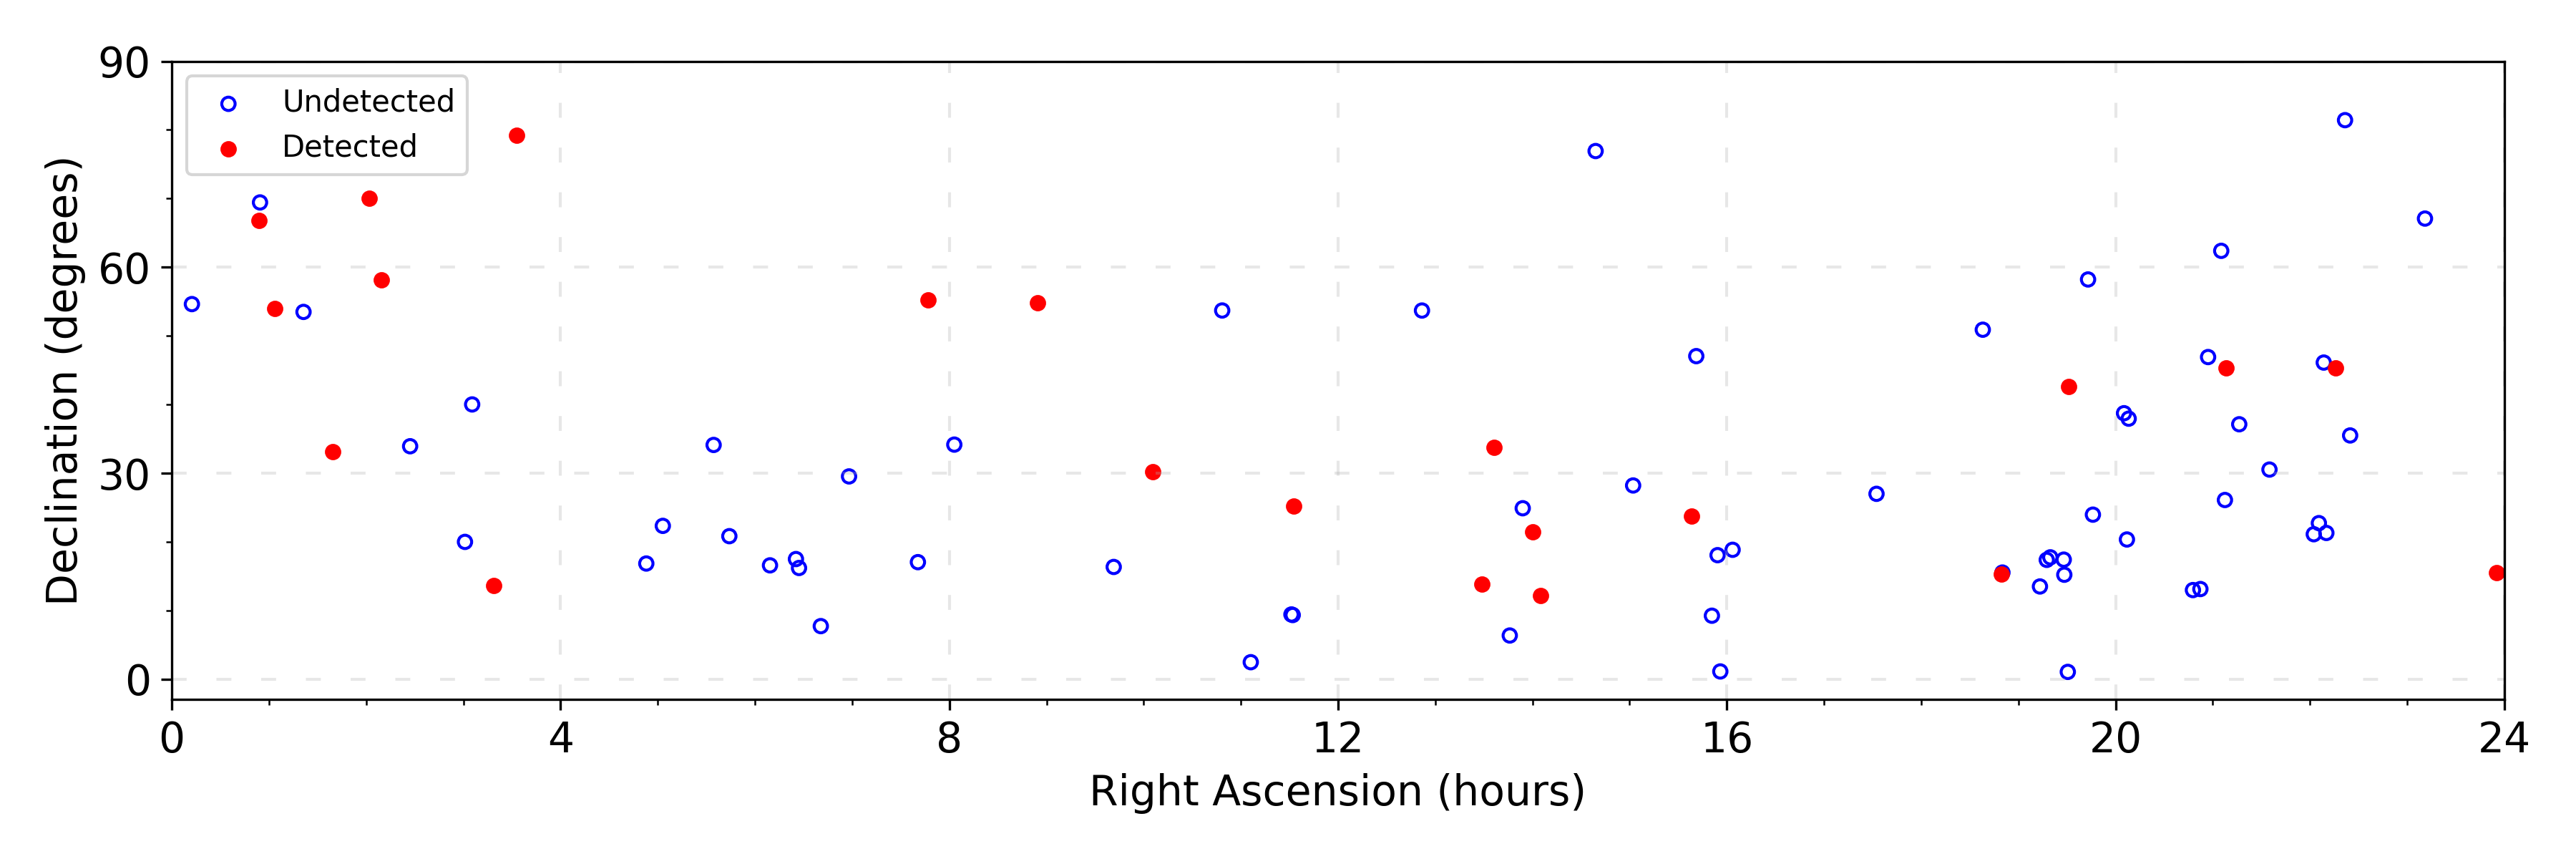
\includegraphics[width=0.92\textwidth]{rrat_observed.png}
%%    \caption[Overview of the sky positions of RRATs observed during RRAT census.]{Overview of the sky positions of the RRATs observed during the census discussed in section \ref{sec:rratsurvey} as of May 2021. Filled red dots indicate sources that have been observed and detected with either single pulses or periodic emission while blue circles indicate sources that were observed but not detected in I-LOFAR data.}
%%    \label{fig:rrat-pc1}
%%\end{figure*}
%%
%%\subsubsection{Pulsars}
%%
%%% ---Pulsar justification---
%%International LOFAR stations are ideal instruments to observe radio pulsars, particularly at frequencies between 100~MHz and 200~MHz \citep{Stappers2011, Bilous2014, Noutsos2015}. Further, the large fractional bandwidth of an international LOFAR station can offer new insight to the spectral variability of giant pulses from the Crab Nebula. Many international stations regularly participate in pulsar studies \citep[for example,][]{Mereghetti2016, Bondonneau2017, Hermsen2018, Donner2019}, while pulsar observations with LOFAR core stations \citep[for example,][]{Bilous2014, Bilous2020} are also common. Recent observations with the Polish international stations include those by \cite{Blaszkiewicz2020}. 
%%
%%To date, over 50 different pulsars have been observed with I-LOFAR using REALTA. Figure \ref{fig:pulsar-pc1} shows a sample of 19 pulsars which were observed, each for 6 minutes, on the 4th and 5th of March 2020, processed using the methods discussed in section \ref{sec:pulsarproc}. In addition, as a result of regular timing campaigns of these sources, a number of targets have been studied in more depth, the Crab Nebula being the prime example. 
%%
%%While the recording and timing of folded profiles of the Crab pulsar are of interest for studying the interior structure of the neutron star via its glitches \citep{Lyne2015} and variability due to scattering and echo events, it also frequently emits so-called `giant pulses' \citep{Meyers2017}. These giant pulses have fluences that vary from hundreds of Jy\,ms to tens of thousands of Jy\,ms. These pulses can be studied to analyse their scintillation, scattering, and brightness distributions.
%%
%%One such example of these giant pulses can be seen in an observation taken of the Crab pulsar with I-LOFAR on 30 June 2020. The observation was processed using the previously described methodology (section \ref{sec:baseproc}, section \ref{sec:pulsarproc}) on REALTA and a short segment of the observation is shown in Figure \ref{fig:giant_pulse}. The figure is made from Stokes I data, where each channel has a bandwidth of 24~kHz and an underlying time resolution of 40.96~$\mu$s (though it has been interpolated using a median filter for this plot). There were $\sim 1300$ giant pulse candidates detected in the 30 minute observation. Using a rate of $\sim 0.7$ giant pulses per second, we determine there are $\sim 20$ giant pulses visible in the dynamic spectrum in the left panel of Figure \ref{fig:giant_pulse}. Other structure in the left panel of Figure \ref{fig:giant_pulse} includes some ionospheric scintillation and RFI. This time segment is mostly of interest due to one rare, extremely bright, giant pulse, which is re-plotted in the right panel of Figure \ref{fig:giant_pulse} where it has been corrected for dispersion effects. Initial analysis using the radiometer equation indicates a specific fluence of $\sim 200$~kJy~ms across the observed bandwidth. Which may be the brightest pulse ever observed for this pulsar at these frequencies \citep{Karuppusamy2012,Meyers2017,VanLeeuwen2020}.
%%
%%As of May 2021, over 80 hours of observations of the Crab pulsar have been captured by REALTA. Initial analysis of this data set, focusing on a four hour observation from March of 2020, has been performed and given results that are similar to that of other low-frequency instruments. The giant pulses were found to form a fluence distribution with a power-law fit of $\alpha = -2.86~\pm~0.07$, similar to that of other low frequency instruments \citep{Meyers2017}, but steeper than the results at Jodrell Bank \citep{Mickaliger2017}. Similarly, an initial investigation of the spectral behaviour of the scattering time scales of the brightest pulses appeared to follow a power law of $\alpha = -3.7 \pm 0.5$, in agreement with other instruments \citep{Driessen2019}. Future work includes planning to integrate a CLEAN-based de-convolution \citep[see][]{Bhat2003} of the pulse shapes to better describe the scattering and dispersion measure variations of single pulses over time, the effects of which are entangled \citep{McKee2018}, especially at lower frequencies.
%%
%%\begin{figure}
%%    \centering
%%    \includegraphics[width=\columnwidth]{quickcrab.png}
%%    \caption[Observation of the Crab Pulsar performed on 30 June 2020.]{Observation of the Crab Pulsar performed on 30 June 2020, (left) without incoherent dedispersion and (right) with incoherent dedispersion. The plot on the left contains several giant pulses and both temporal- and spectral-variable ionospheric scintillation.  The plot on the right focuses on the brightest pulse in the group, which is the brightest pulse observed from the Crab Pulsar with I--LOFAR to date. Here data were processed to channel bandwidths of 24~kHz, resulting in a sampling rate of 40.96$\mu$s. The data were time integrated to a temporal resolution of 1.31~ms prior to plotting.}
%%    \label{fig:giant_pulse}
%%\end{figure}
%%
%%\subsubsection{Rotating radio transients}\label{sec:rratsurvey}
%%Rotating radio transients (RRATs) are a class of neutron star that were discovered through detecting single, bright pulses rather than periodicity searches. If a sufficient number of pulses are detected within a short observing window, it is possible to determine the underlying period of the neutron star through brute force methods, after which the times of arrival of these pulses can be used to time the sources like any other pulsar \citep{Keane2011}. While the LOFAR core has blindly detected several RRATs during the LOTAAS survey \citep{Sanidas2019, Michilli2020, Tan2020}, and through targeted follow-up observations of sources detected with the Green Bank Telescope \citep{Karako-Argaman2015}, there has not been a major undertaking to time these sources with the LOFAR instruments, using the core or international stations.
%%
%%However, the full-sky sensitivity and fractional bandwidth of a single international LOFAR station makes it the perfect candidate to perform follow-up observation on some of the brighter RRAT candidates identified by all-sky monitoring instruments such as the Big Scanning Array of Lebedev Physical Institute (BSA LPI) and the Canadian Hydrogen Intensity Mapping Experiment \citep[CHIME;][]{Amiri2018}. Follow-up observations of these candidates are useful to (a) determine the rotational characteristics of the stars through phase-coherent follow-up timing; and to (b) perform source characterisation from examining stars with broad spectral coverage.
%%
%%Between July 2020 and May 2021, a 500 hour observing campaign has been undertaken to observe a diverse set of RRATs from the RRatalog\footnote{\hyperref[RRatalog]{http://astro.phys.wvu.edu/rratalog/}}, the CHIME-FRB Galactic sources database\footnote{\hyperref[CHIME-FRB Galactic Sources]{https://www.chime-frb.ca/galactic}}, and the BSA LPI Transients Catalogue\footnote{\hyperref[BSA LPI Transients Catalogue]{https://bsa-analytics.prao.ru/en/transients/rrat/}}, with a focus on sources that as yet do not have well defined periods. An overview of the sources observed and detected by this census can be seen in Figure \ref{fig:rrat-pc1}. This campaign has so far resulted in the discovery of rotation periods for two sources which were previously unknown, periodic detection of a further two sources that have not been previously detected at LOFAR frequencies and the determination of coherent timing solutions for thirteen other sources. These results will be discussed in detail in a future paper (McKenna et al. in prep).%\citep{McKenna2021}.
%%
%%
%%\subsubsection{Fast radio bursts}
%%Since their discovery in 2007 by \citeauthor{Lorimer2007}, fast radio bursts (FRBs) have been of keen interest to radio astronomers across the globe. While blind searches with multiple telescopes have helped push the lower bounds of their emission frequencies down year on year, the detection of numerous repeating FRBs by the CHIME-FRB collaboration \citep{CHIME2019} has accelerated this process in recent months. Searches for FRBs with LOFAR include those by \cite{Karastergiou2015} and \cite{TerVeen2019}, for example.
%%
%%One particular repeating FRB, FRB 20180916B (`R3') has been found to have a period of $16.35\pm 0.15$ days, with an activity window of 5 days \citep{Amiri2020}, and has been detected with the LOFAR core as of December 2020 \citep{Pastor-Marazuela2020, Pleunis2021}. Prior to this, I-LOFAR and REALTA were used as a part of a 70 hour campaign to observe R3 during its activity phase and attempt to see emission at previously unseen frequencies. However, no significant pulse candidates were detected during this campaign. For further results and observations of other FRB sources see McKenna et al. (in prep).
%
%\subsubsection{Solar radio bursts}
%Solar radio bursts (SRBs) are some of the brightest phenomena in the radio sky. Five types of SRBs were classified in the 1950s \citep{Wild1950b, Boischot1957, Wild1959} and have been studied regularly since \citep[See][for a comprehensive review]{Pick2008}. A number of observations of solar radio bursts have been taken either using the LOFAR array as part of the Solar and Space Weather KSP \citep[for example,][]{Zhang2020, Murphy2021} or with an international station during local mode \citep[for example,][]{Morosan2019, Maguire2020, Bartosz2020}. Most solar radio bursts occur due to the plasma emission process, first described by \cite{Ginzburg1958}, and as such can be used as a diagnostic for the plasma density in the solar corona \citep{Melrose1987}. Remote sensing of radio emission from the Sun can be used as diagnostics of both large scale energy release from solar flares and CMEs \citep{Carley2021} and small-scale energy release, potentially related to coronal heating \citep{Mondal2020}.
%
%On 2 November 2020, I-LOFAR observed a solar radio noise storm in mode 357. The dynamic spectrum of this storm from 12:00 - 14:00 UTC is shown in Figure \ref{fig:357_10ms}a at 10~ms temporal resolution and \SI{195.3125}{\kilo \hertz} spectral resolution. A large number of short duration SRBs are seen across the full HBA band. Fine scale temporal and spectral structure are thought to be indicative of the turbulent nature of the solar corona which could further enhance the diagnostic capability of SRBs \citep{Kolotkov2018, Sharykin2018, Reid2021}.
%
%\begin{figure}
%    \centering
%    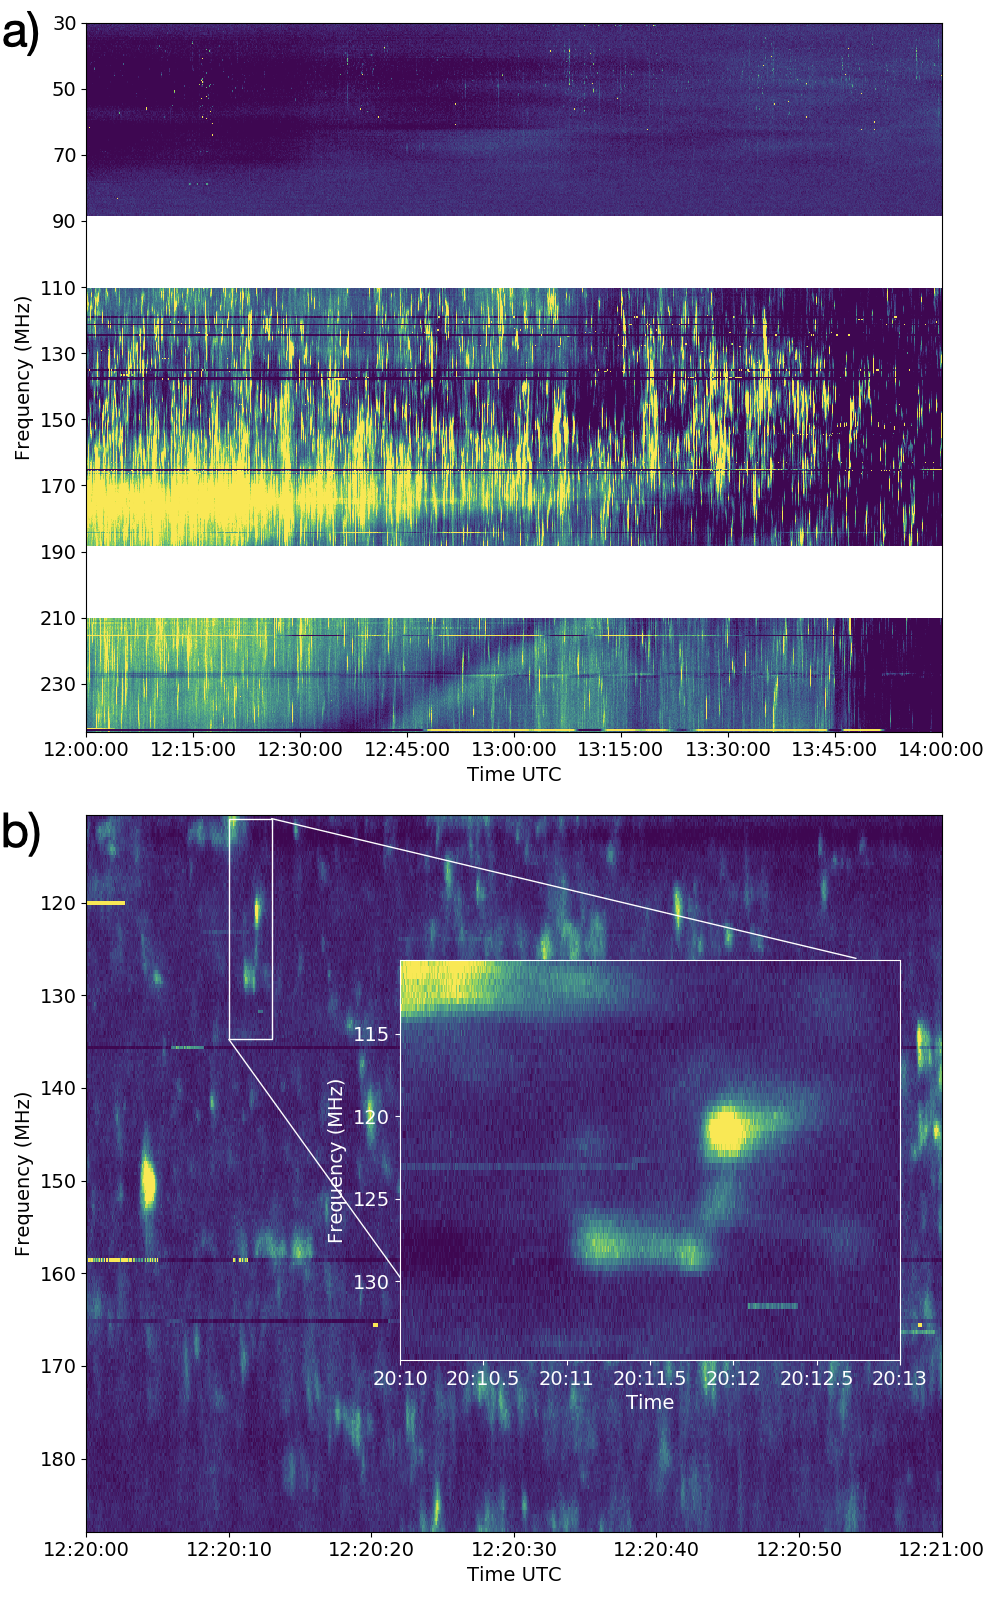
\includegraphics[width=0.75\columnwidth]{bursts.png}
%    \caption[Solar radio noise storm observed on 2 November 2020.]{Solar radio noise storm observed on 2 November 2020. a) In this mode 357 observation, a number of bright bursts can be seen at frequencies greater than 110~MHz (yellow in the dynamic spectrum). %\SIrange{110}{190}{\mega\hertz}
%    Here the data spans 2 hours from 12:00 UTC and has a temporal resolution of 10~ms.
%    %\SI{10}{\milli \second}. 
%    b) Zoom-in of panel a at 1~ms temporal resolution. A number of short duration SRBs are observed. The inset shows the sub-second variation of an individual burst in the noise storm, also at a temporal resolution of 1~ms.}
%    \label{fig:357_10ms}
%\end{figure}
%
%Some SRBs can exhibit fine scale temporal and spectral features. These include, for example, herringbone bursts which are observed as part of Type II bursts \citep[for example,][]{Carley2015} or individual striations of a Type IIIb burst \citep[for example,][]{Zhang2020}. 
%A number of short duration radio bursts, which are not part of the five classified types, have also been reported \citep[for example,][]{Ellis1967, Ellis1969, Melnik2010}. 
%The high temporal resolution of REALTA observations with I-LOFAR will allow the study of these bursts at some of the highest temporal resolutions to date. Figure \ref{fig:357_10ms}b shows a zoom-in of the radio noise storm from Figure \ref{fig:357_10ms}a at 1~ms temporal resolution with an inset showing the sub-second variation of a particular burst. Figure \ref{fig:uburst} shows an LBA observation from 2 June 2020 of a Type III burst and a U burst, both described by \cite{Reid2014}, for example, as being generated by electron beams travelling along open and closed magnetic field lines away from the sun respectively. This observation also has a 1~ms temporal resolution. Although a single international LOFAR station can only make spectroscopic observations of Type III bursts and their sub-types, this is still a valuable tool in determining the characteristics of the accelerated electron beam that instigates plasma emission in these bursts \citep{Reid2018}. Further, short duration pulsations in radio bursts can give insight into magnetohydrodynamic oscillations in the solar corona \citep{Carley2019}.
%
%\begin{figure}[ht]
%    \centering
%    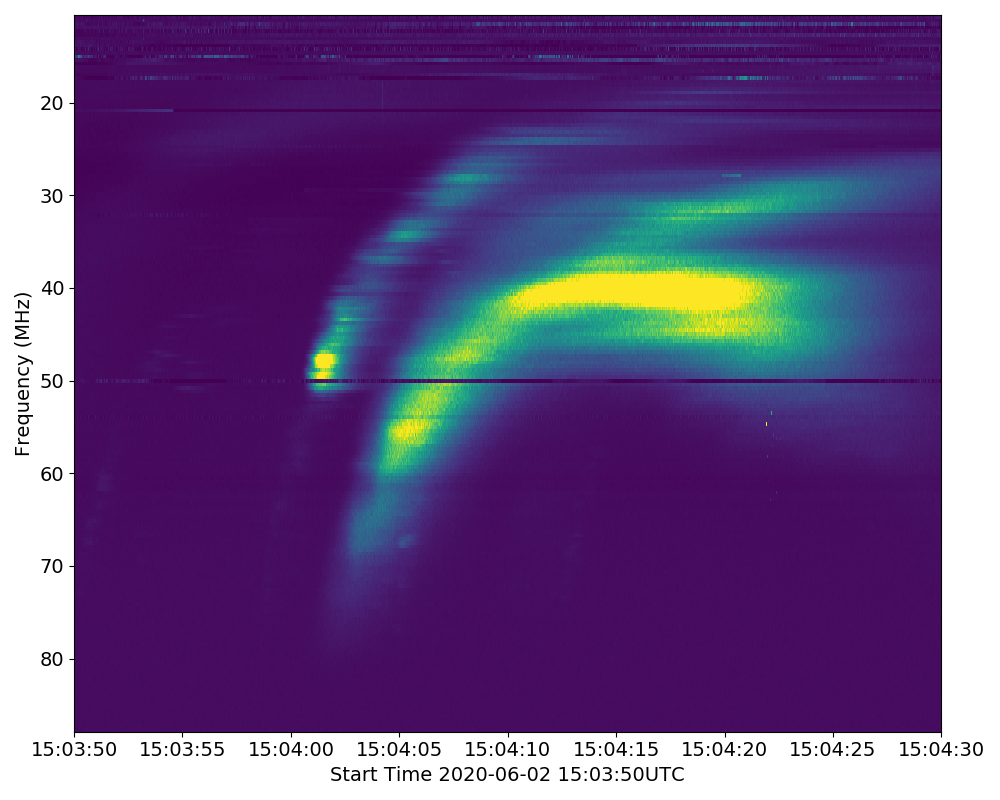
\includegraphics[width=\columnwidth]{Uburst_1ms_1090MHz.png}
%    \caption[Two solar radio bursts observed on 2 June 2020.]{Two solar radio bursts observed on 2 June 2020. The earlier burst is likely a Type III SRB while the later burst shows the morphology typical of a U burst. The observation has a spectral resolution of $\sim$ \SI{195}{\kilo \hertz} and a temporal resolution of \SI{1}{\milli \second}.}
%    \label{fig:uburst}
%\end{figure}
%
%%\subsubsection{Jovian auroral radio emission}
%%
%%%\begin{figure}
%%\begin{figure*}[t]
%%    \centering
%%%       \includegraphics[width=\columnwidth]{Jupiter_Io_IE613.png}
%%        \includegraphics[width=\columnwidth]{Jupiter_Io_IE613.png}              
%%    \caption[Observation of a Jovian Decametric emission produced by the Io-Jupiter interaction.]{Observation of a Jovian Decametric emission produced by the Io-Jupiter interaction. Panel (a) shows Stokes I (in dB above background). Panel (b) displays Stokes V (in arbitrary units). The resolution is $84$~ms per $12.2$~kHz. The emission displays a strong negative value in Stokes V, which means a strong right-hand circular polarization. Panels (c) and (d) show respectively a $60$~s and $10$~s zoom-in of panel (a) (Stokes I), processed with the highest resolution available for this observation ($81.92$~$\mu$s per $12.2$~kHz). Millisecond drifting bursts are visible panel (d).}
%%    \label{fig:io-stokesI}
%%\end{figure*}
%%
%%
%%%After solar radio bursts, Jupiter's decametric emission (DAM) is the most intense radio emission in our solar system.  the Jovian DAM extends above the ionospheric cutoff frequency to a maximum of $\approx$ 40~MHz, and have been observed from the ground since the 1950s \citep{Burke1955}.
%%%Jupiter's decametric emission (DAM) has been observed from the ground since the 1950s \citep{Burke1955}. 
%%Decametric radio emission (DAM), the strongest component of Jovian auroral radiation, was discovered in 1955 by \cite{Burke1955}, with part of this emission controlled by the Io-Jupiter interaction \citep{Bigg1964}. The source of this radio emission is known to be due to the electron cyclotron maser instability (ECMI) in the Jovian magnetosphere, which occurs when a circularly polarised wave resonates with the gyration of electrons with relativistic energies \citep{Wu1979,Wu1985,Zarka1998, Treumann2006,Louarn2017GRL}. The ECMI amplifies the wave on the extraordinary R-X mode which can escape the source and propagate in free space as a radio wave, at a frequency very close to the local electron cyclotron frequency, which is proportional to the local magnetic field amplitude. Jovian DAM emissions are the only planetary radio emissions visible from the ground, since part of the DAM is emitted at a frequency above the ionospheric cutoff frequency ($\gtrsim 10$~MHz). BF observations of Jovian DAM using the LOFAR core stations have been used to test the sensitivity of LOFAR to exoplanetary radio emissions \citep{Turner2019, Turner2021}.
%%
%%%On 13 October 2020, I-LOFAR detected observed Jovian DAM emission from 17:41:30 to 18:00:00 UTC. The Stokes I data from this observation is shown in Figure \ref{fig:io-stokesI} panels a and b while Stokes V for the period 17:47:00 - 17:57:00 UTC is shown in Figure \ref{fig:io-stokesI} panel c. Given this is Jovian DAM emission, the magnetic field of Jupiter can be probed through the relationship $\nu_{\rm MHz} = 2.8 B_{G}$. This gives a first order estimation of Jovian magnetic field, for which we cannot infer an altitude without a magnetospheric model, from $\approx 8$\textendash$11$ G ($22$\textendash $31$ MHz) as the electrons traverse along magnetic field lines in the magnetosphere. In order to know the exact position of the sources, it is necessary to make interferometric measurements with several LOFAR stations. \par
%%
%%On 8 June 2021, I-LOFAR observed Jovian DAM emission produced by the Io-Jupiter interaction, from 04:10 to 05:30 UTC. The Stokes I and V data from this observation are shown in Figure \ref{fig:io-stokesI}a-b. An arc shape emission with a high intensity is observed between $\sim 04$:$55$ and $05$:$30$ (corresponding to the main Io-DAM emission), preceded by emissions with lower intensity starting at $\sim 04$:$10$ (corresponding to secondary Io-emissions). Looking at both the shape of the emission and its polarization (strong negative Stokes V value, corresponding to a right-handed circular polarization), we can determine that this emission is an Io-B emission \citep[coming from the north-dawn side of Jupiter, see][for example]{Marques2017}.
%%
%%Moreover, we have with I-LOFAR access to very high temporal and frequency resolution, of which an example is shown Figure \ref{fig:io-stokesI}c,d ($81.92$~$\mu$s per $12.2$~kHz). This will allow us to study the microphysics of the Jovian decametric emissions, for example the millisecond bursts visible Figure \ref{fig:io-stokesI}d with a drifting feature in frequency with time ($\sim 25$-$30$~MHz). These millisecond drifts are thought to be electron bunches propagating along the magnetic field lines and can reveal both the energy of the resonant electrons as well as the potential drops (if present) along these fields lines \citep{Hess2007, Hess2009}. The high-resolution capability will also enable constraints to be placed on the position and movement of the sources, by interferometric measurements with several LOFAR stations, as well as the characteristics of the emission (for example, thickness and opening of the emission beam). Finally, I-LOFAR, combined with REALTA, is equipped to join the other LOFAR stations in the ground radio observation campaigns in support of the Jupiter space missions, both current (Juno\footnote{Such as the Juno Ground Radio Observation Support \hyperref[Juno]{https://maser.lesia.obspm.fr/task-1-data-collections/juno-ground-radio/}}) and future (JUICE, Europa-clipper).
%
%%One could note that no such intense emission has been observed by the Nan\c{c}ay Decametric Array \citep[NDA;][]{Boischot1980} during the same time period and frequency range, which demonstrates the ability of I-LOFAR to observe high-time resolution low-frequency radio emissions from the Jovian magnetosphere (with REALTA to process the data), which are not detectable by other low-frequency radio telescopes. During this observation, Jupiter was not ideally placed in the sky, reaching a maximum of 11$^{\circ}$ in elevation. Since the sensitivity increases with the target elevation, observations of Jupiter at a higher elevation will give a higher Signal-to-Noise Ratio. Under favourable conditions, Jupiter can reach $\sim$ \textbf{58 degrees elevation for example, at opposition in December 2024}. Using a Hamaker beam model from \texttt{dreambeam} \cite{Carozzi2016}, we estimate a 95\% reduction in sensitivity at the currently observed elevation.\par
%%The I-LOFAR LBA is 40 times more sensitive than the NDA \citep{Clarke2014}, and so it is not surprising that the NDA did not detect this particular DAM emission.
%
%%the microphysics of these emissions (such as the frequency drift, the possibility of distinguishing multiple emissions).
%
%
%
%
%
%
%
%
%%\subsubsection{SETI}
%%International LOFAR stations such as I-LOFAR have very broad fields of view, particularly at frequencies less than 150~MHz \citep{VanHaarlem2013}. This, coupled with the ability to channelise data to bandwidths $\lesssim 1$~Hz, are favourable characteristics in SETI research.
%%BL is conducting one of the most sensitive, comprehensive, and intensive searches for technosignatures on other worlds across a large fraction of the electromagnetic spectrum \citep{Worden2017}. Targets of the BL program include one million nearby stars, one hundred nearby galaxies, the entire Galactic plane, and exotic astrophysical objects \citep[see][for detail]{Isaacson2017}. \cite{Gajjar2019} provides the current status of these observing campaigns, as well as listing a number of collaborative observing facilities that are working alongside BL for carrying out these sensitive studies. The BL program is collaborating with two of the international LOFAR stations: I-LOFAR and LOFAR-SE, which is located at Onsala (Sweden), to complement searches towards the above-mentioned BL targets at lower radio frequencies. Details of the dedicated hardware deployed at I-LOFAR is discussed in section \ref{sect:pipeline_SETI}. First-light observations were conducted with these BL nodes on 19 November 2020 towards PSR B1919+21 to validate the BL recording and conversion pipelines.
%%Recently, we also conducted observations of PSR B2217+47 on 21 April 2021 using the BL nodes for further pipeline development. Baseband data in the GUPPI format were converted to two different temporal and spectral resolution total intensity \texttt{SIGPROC} formatted filterbank data products. PSR B2217+47 was clearly detected, by folding high-temporal products. To search for narrowband Doppler drifting signals, \texttt{SIGPROC} formatted filterbank files with 3~Hz spectral resolution were used. This made use of the BL narrowband signal search tool, \texttt{turboSETI} \citep{Enriquez2017}. Figure \ref{fig:BL_fig} shows an example of one of the narrowband signals of terrestrial origin detected using \texttt{turboSETI} towards PSR B2217+47. In the future, it is planned to conduct detailed on-target and off-target observations to discriminate such anthropogenic signals from true sky-bound ETI signals. 
%%
%%
%%\begin{figure}
%%    \centering
%%    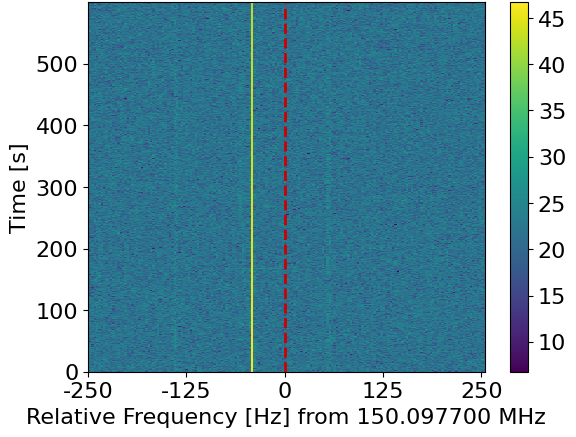
\includegraphics[width=\columnwidth]{B2217+47_crop.png}
%%    \caption[Narrowband signal detected using REALTA and the \texttt{turboSETI} algorithm.]{Narrowband signal detected using REALTA and the \texttt{turboSETI} algorithm. Dynamic spectra of an example narrowband signal detected in an observation pointing toward PSR B2217+47 using \texttt{turboSETI} with the BL nodes in REALTA. The colour bar shows intensity in arbitrary units while the red dotted line shows a relative frequency of 0~Hz from 150.0977~MHz. The signal does not show any drifting and thus likely has a terrestrial origin.}
%%    \label{fig:BL_fig}
%%\end{figure}
%
%
%\subsection{Future development of REALTA}
%\label{sec:realta_future_work}
%
%Here I have described the hardware for REALTA and given an overview of the software used to record and analyse data recorded from I-LOFAR. First observations of solar radio bursts were showcased, while the broad range of objects that I-LOFAR and REALTA can observe can be seen in \cite{Murphy2021b}. 
%
%LOFAR 2.0 is a series of hardware and software upgrades to the ILT, which will be implemented in a number of stages over the coming years. An upgrade to an international LOFAR station, such as I-LOFAR, will require new receiver units (RCU2), new station beamformers (Station Digital Processors) based on the Uniboard$^2$ architecture \citep{Schoonderbeek2019} and new power, clock and control board for improved station control. The upgrade will greatly improve the instantaneous bandwidth, sensitivity and RFI rejection of an international station.
%
%%The ability to observe using both the LBAs and HBAs simultaneously effectively doubles the data rate of a LOFAR station ($\sim 6.4$~Gbps) and will require a sufficiently high speed network and recording system to record the raw data.
%%Two major upgrades to LOFAR are \textbf{due to be completed} in the coming years, namely, LOFAR2.0 \textbf{stage 1}\footnote{\hyperref[LOFAR2.0]{https://www.glowconsortium.de/index.php/en/lofar-about/lofar-2-0}} and Space Weather (LOFAR4SW\footnote{\hyperref[LOFAR4SW]{https://www.lofar4sw.eu}}). The LOFAR2.0 \textbf{stage 1 } upgrade is a major hardware and software upgrade to LOFAR's station electronics including the receiver units and digital processing systems. A LOFAR2.0 station will be able to observe using both the LBAs and HBAs simultaneously, significantly increasing the data output of an international LOFAR station. For upgraded international stations, the increased data rate necessitates a dedicated telescope backend such as REALTA to capture and pre-process the raw voltages in stand-alone mode. 
%
%LOFAR for Space Weather (LOFAR4SW) \footnote{\hyperref[LOFAR4SW]{http://www.lofar4sw.eu}} is a proposed upgrade to LOFAR, currently being designed to enable regular space weather monitoring. If completed, LOFAR4SW would allow near-real-time monitoring of space weather phenomena such as solar flares and coronal mass ejections, interplanetary scintillation and ionospheric disturbances \citep{Carley2020}. This is useful not only to space weather researchers but to the radio astronomy community as a whole as it will broaden our understanding of how space weather can effect the propagation of radio waves in the inner heliosphere and disturbances in the ionosphere and the effect this has on observing astronomical sources. In order to record the data streams from a LOFAR4SW enabled international station in local mode, a backend such as REALTA will be required to capture the data-stream and to process the raw data so that it can be used by space weather researchers and forecasters. The effectiveness of machine learning algorithms to detect solar radio bursts with REALTA is currently being investigated.
%
%In the future, REALTA will be upgraded to fully include the BL headnode into the system. In order to achieve this, additional VLAN fibre connections will be set up between the UCC compute nodes and the BL headnode and compute nodes. Activating these VLAN fibre connections will allow each machine to record one lane of data and perform real-time channelisation and dedispersion making use of their GPUs.  The BL headnode will distribute an identical OS to the UCC and BL compute nodes and control them in parallel. This will allow REALTA to monitor for radio transients such as those important to SETI research. Upgrades to the data preparation and processing stages of the REALTA data flow (Figure \ref{fig:REALTA_future}) will see REALTA operating fully in real-time (see section \ref{sec:future_software}). %In addition, we are working with Kx Systems developers to create a next-generation system that harnesses the power of kdb+, the fastest time--series database for rapid, real-time data ingestion and processing \footnote{\hyperref[Kx] https://kx.com/blog/dias-kx-and-i-lofar-new-windows-on-the-universe-through-software/}.  
%
%With future upgrades to ILT hardware coming in the first half of the 2020s \citep[mainly, LOFAR2.0;][]{Edler2021}, international LOFAR stations will require a dedicated high-performance backend to record data rates of $\sim$6.4~Gbps, should they wish to use the full capacity of the instrument in local mode. While some international stations have existing backends, REALTA offers a powerful backend that is well suited to the data rates of LOFAR2.0. Backends like REALTA, due to the use of commercially available hardware, straight-forward network configuration and freely available software, will make it possible for international LOFAR stations to capture and process raw data, and to undertake a wider variety of astronomical observations. As mentioned in section \ref{sec:future_software}, in the future it will be possible to process and record raw data in real-time. This will be done by recording data to a ring buffer implemented with the Parkes-Swinburne Recorder Distributed Acquisition and Data Analysis software \citep[PSRDADA;][]{PSRDADA} and then reading from the ring buffer into \texttt{udpPacketManager}. This will further improve the capabilities of international LOFAR stations during local mode. Finally, cooperation and coordinated observations between international LOFAR stations becomes easier if using the same software and hardware for data capture and post-processing and will be more beneficial than each international station operating individually.
%
%As LOFAR is primarily used for its interferometric imaging, I now describe the mathematical background for radio interferometry and outline a common deconvolution algorithm used to create images. 

\section{Radio Interferometry}
\label{sec:interferometry}
Rayleigh's criterion states that for an object to be resolved, the maximum of its interference pattern must overlap the minimum of another. This leads to the mathematical relationship (assuming a circular aperture), 
$$\theta \approx 1.22 \frac{\lambda}{D}$$ 
where $\theta$ is the angular resolution of an object, $\lambda$ is the wavelength observed in and $D$ is the aperture diameter of the telescope. For telescopes observing optical wavelengths, this limit is often superseded by the ``seeing" of the atmosphere. Adaptive optics help overcome this challenge and bring optical telescopes close to the diffraction limit. For radio telescopes at low frequencies, the challenge becomes one of structural engineering. For a radio telescope observing at 30 MHz to have a similar resolution to the Hubble Space telescope, for example, it would need an aperture diameter of 41,000 km. Fortunately, two radio antennas placed some distance apart has the same angular resolution as single dish with the same diameter. This technique is known as radio interferometry and to explain how it works I first discuss the coherence of the electric field of an astronomical object before introducing the most fundamental radio interferometer, the two element interferometer.

An astronomical object at some position $\mathbf{R}$ radiating radio electromagnetic waves with a time variable electric field of the form $\mathbf{E}(\mathbf{R}, t)$ is observed by an astronomer at some point $\mathbf{r}$. In order to disregard the time variable nature of the electric field we consider only the coefficients of the Fourier series of $\mathbf{E}(\mathbf{R}, t)$ which we denote as $\mathbf{E}_\nu (\mathbf{R})$, the quasi-monochromatic components of $\mathbf{E}(\mathbf{R}, t)$ at frequency $\nu$, and note that these are complex values \citep{synthesisimaging1999}.	We make the assumption that the object is sufficiently far away so that the field strength of the source can be described as the field strength on some imaginary ``celestial sphere" with radius $R = \vert \mathbf{R} \vert$ within which there is no additional radiation. The field strength observed at $\mathbf{r}$ can be expressed in terms of the field strength on this sphere, $\mathcal{E}_\nu (\mathbf{R})$, via
\begin{equation}
\label{eq:int_fieldstrength}
E_\nu(\mathbf{r}) = \int \mathcal{E}_\nu (\mathbf{R}) \frac{e^{2\pi i \nu \vert \mathbf{R} - \mathbf{r} \vert/c}}{\vert \mathbf{R} - \mathbf{r} \vert} dS,
\end{equation}
where $dS$ is the surface area element on the celestial sphere. The correlation of the field at two points $\mathbf{r}_1$ and $\mathbf{r}_2$ is defined as $\mathsf{V}_\nu (\mathbf{r}_1, \mathbf{r}_2) = \langle E_\nu(\mathbf{r}_1) E^{*}_\nu(\mathbf{r}_2) \rangle$, where the asterisk denotes the complex conjugate. Substituting in Equation \ref{eq:int_fieldstrength} gives
\begin{equation}
\label{eq:int_correlation}
\mathsf{V}_\nu (\mathbf{r}_1, \mathbf{r}_2) = \bigg \langle \int \int \mathcal{E}_\nu(\mathbf{r}_1) \mathcal{E}^{*}_\nu(\mathbf{r}_2) 
\frac{e^{2\pi i \nu \vert \mathbf{R}_1 - \mathbf{r}_1 \vert/c}}{\vert \mathbf{R}_1 - \mathbf{r}_1 \vert} \frac{e^{-2\pi i \nu \vert \mathbf{R}_2 - \mathbf{r}_2 \vert/c}}{\vert \mathbf{R}_2 - \mathbf{r}_2 \vert} dS_1 sS_2 \bigg \rangle.
\end{equation}
If we assume that the radiation from the astrophysical source is spatially incoherent, then  $\langle \mathcal{E}_\nu(\mathbf{r}_1) \mathcal{E}^{*}_\nu(\mathbf{r}_2) \rangle = 0$ for $\mathbf{R}_1 \neq \mathbf{R}_2$ and Equation \ref{eq:int_fieldstrength} can be simplified to  

\begin{equation}
\label{eq:int_correlation2}
\mathsf{V}_\nu (\mathbf{r}_1, \mathbf{r}_2) =  \int \langle \vert \mathcal{E}_\nu(\mathbf{r})^2 \vert \rangle \vert \mathbf{R} \vert^2
\frac{e^{2\pi i \nu \vert \mathbf{R} - \mathbf{r}_1 \vert/c}}{\vert \mathbf{R} - \mathbf{r}_1 \vert} \frac{e^{-2\pi i \nu \vert \mathbf{R} - \mathbf{r}_2 \vert/c}}{\vert \mathbf{R} - \mathbf{r}_2 \vert} dS.
\end{equation}
By introducing the unit vector $\mathbf{s} = \mathbf{R}/ \vert \mathbf{R} \vert$ and writing the observed intensity $I_\nu(\mathbf{s}) = \mathcal{E}_\nu(\mathbf{r})^2 \vert \rangle \vert \mathbf{R} \vert^2$ and ignoring terms of order $\vert \mathbf{r}/\mathbf{R} \vert$ we finally arrive at a useful form of $\mathsf{V}_\nu (\mathbf{r}_1, \mathbf{r}_2)$

\begin{equation}
\label{eq:int_correlation_final}
\mathsf{V}_\nu (\mathbf{r}_1, \mathbf{r}_2) \approx \int I_\nu(\mathbf{s}) e^{-2 \pi i \nu\mathbf{s} \cdot (\mathbf{r}_1 - \mathbf{r}_2)/c} d\Omega,
\end{equation}
where the surface element $dS$ is given by $\vert \mathbf{R} \vert ^2 d\Omega$.

The most important conclusion to draw from Equation \ref{eq:int_correlation_final} is that it depends only on the distance between the two points, not their absolute position. Thus, $\mathsf{V}_\nu (\mathbf{r}_1, \mathbf{r}_2)$ can be determined from only one pair of points. The function $\mathsf{V}_\nu$ for a single separation $\mathbf{r}_1 - \mathbf{r}_2$ is called the spatial coherence function and is all that needs to be measured to study the emitting astronomical source.

\begin{figure}[ht]
    \centering
    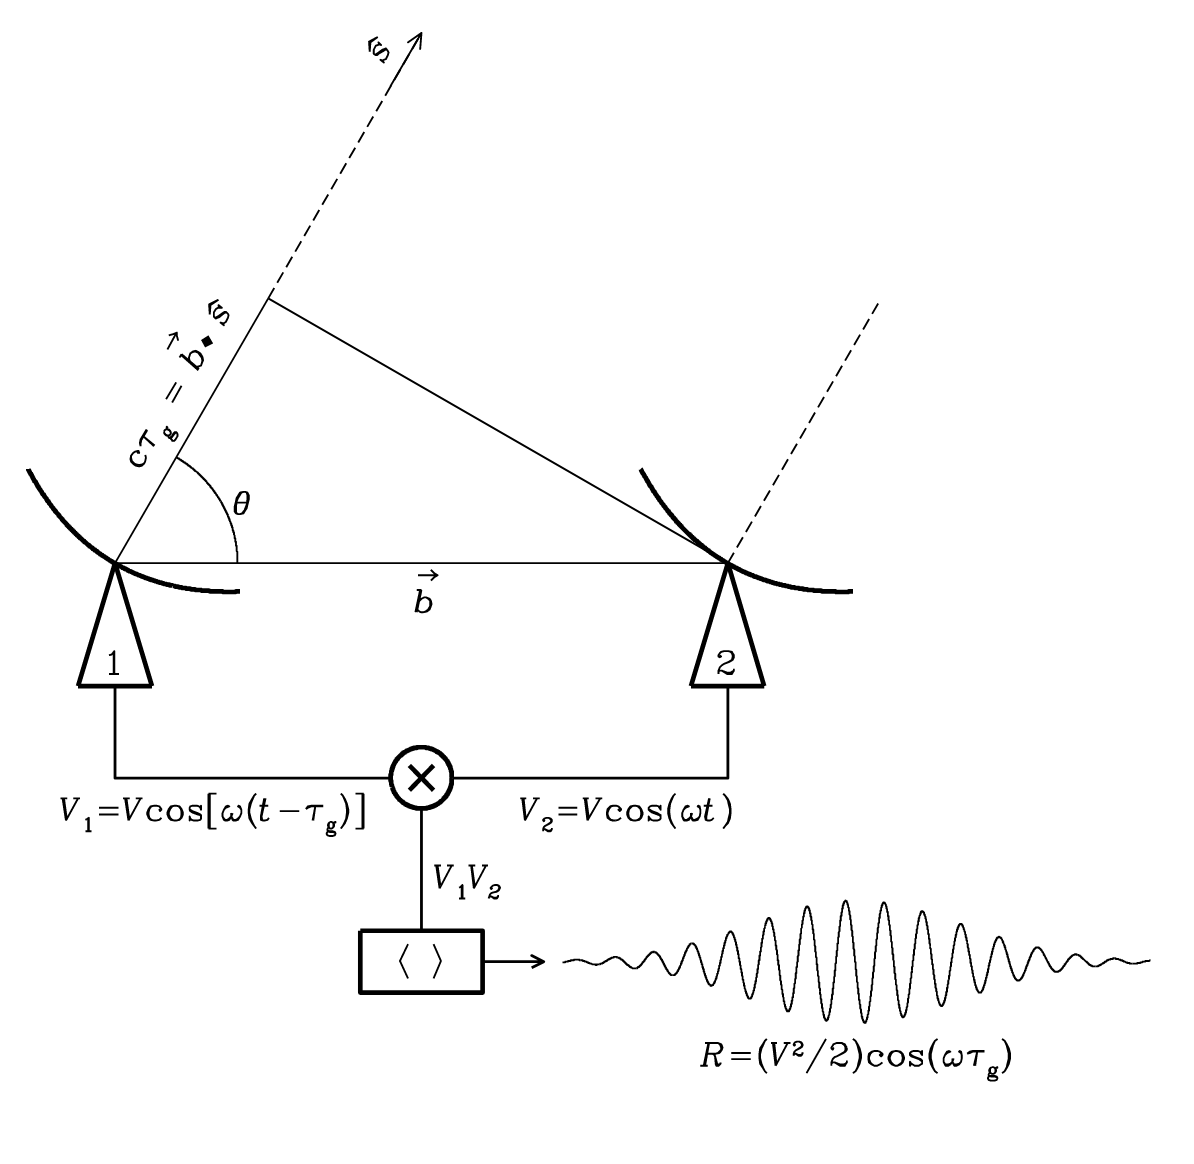
\includegraphics[width=0.75\columnwidth]{Images/2_elem_int.png}
    \caption[A two element interferometer]{A two element interferometer separated by a baseline $\overrightarrow{\Vec{b}}$. The signal from each antenna is correlated by first multiplying the two voltages then time averaging them.}
    \label{fig:2_el_int}
\end{figure}

How then does one measure the spatial coherence function? Let's imagine putting two radio antennas (antenna 1 and antenna 2) at points $\mathbf{r}_1$ and $\mathbf{r}_2$. The vector distance between these antennas is given by $\overrightarrow{\Vec{b}} = \mathbf{r}_1 - \mathbf{r}_2$. As shown in Figure \ref{fig:2_el_int}, a radio wave approaching the antennas from direction $\hat{\Vec{s}}$  will hit antenna 2 first then antenna 1 after a time delay of $\tau_g$ such that,
\begin{equation}
\label{eq:time_delay}
\tau_g = \frac{\overrightarrow{\Vec{b}} \cdot \hat{\Vec{s}}}{c}
\end{equation}
where $c$ is the speed of light. The output from each antenna is a voltage $V_1 = V \cos{\omega(t - \tau_g)}$ and $V_2 = V\cos{\omega t}$. 


The total response, $R_c$ of the interferometer is the correlation or multiplication and time average of these two voltages, $\langle V_1 V_2 \rangle$. 
$$
R_c = \langle V_1 V_2 \rangle = \frac{V^2}{2} \cos{\omega \tau_g}
$$
Furthermore, if a 90$^\circ$ phase shift is added to the output of one antenna, the response becomes
$$
R_s = \langle V_1 V_2 \rangle = \frac{V^2}{2} \sin{\omega \tau_g}.
$$
A complex visibility can be defined as the complex sum of the two responses $V(\hat{\Vec{s}}) = R_c - iR_s$. Using Euler's formula, the complex visibilty of an extended source, at a particular frequency, is given by:
\begin{equation}
\label{eq:complex_vis}
V_\nu(\hat{\Vec{s}}) = \int I_\nu(\hat{\Vec{s}}) \exp{(-i \omega \tau_g)} d\Omega = \int I_\nu(\hat{\Vec{s}}) \exp{(-2 \pi i \frac{\overrightarrow{\Vec{b}} \cdot \hat{\Vec{s}}}{\lambda}}) d\Omega
\end{equation}
where $I_\nu$ is the sky brightness distribution at frequency $\nu$. Notice now how Equation \ref{eq:complex_vis} is identical to Equation \ref{eq:int_correlation_final} once it has been rewritten in terms of wavelength. Thus, the output of a complex correlator \textit{is} the spatial coherence function!

We now choose a convenient coordinate system to describe this measurement. In this coordinate system, the separation between antennas is measured in terms of wavelength $\mathbf{r}_1 - \mathbf{r}_2 = \lambda(u, v, w=0)$ and the components of the unit vector $\mathbf{s}$ become $(l, m, n = 1)$. In this \textit{uvw} coordinate system, $d\Omega$ becomes $dl dm$ and Equation \ref{eq:complex_vis} becomes

\begin{equation}
\label{eq:complex_vis_uvw}
V_\nu(u,v) = \int I_\nu(l,m) e^{-2 \pi i (ul + vm)} dl dm
\end{equation}

Here we see that the complex visibility (a.k.a spatial coherence function) is the Fourier transform of the sky brightness distribution.

%Equation \ref{eq:complex_vis} can be rewritten as a function of the \textit{uvw} coordinate system and using the directional cosine coordinate system for source position on the sky.

% their phase information can be recorded. Thus, multiple, smaller radio antenna placed at great distances will obtain the same resolution as a single dish. such that $\overrightarrow{\Vec{b}} \cdot \hat{\Vec{s}} =b\cos \theta$
Before describing how to invert this Fourier transform, I take a moment to describe the \textit{uvw} coordinate system a bit further.
As we saw, the components of the unit vector $\mathbf{s}$ of the source in the sky are given by \textit{(l,m,n)}. These are directional cosines and determine a position on the sky in terms of the direction cosines to that position. First we introduce the concept of a \textit{phase centre}, a position on the sky to which the main response of the antennas is pointed either by physically steering the antennas or introducing appropriate phase delay in the correlation described above.
\textit{l,m,n} can then be defined as
\begin{align*}
l &= \cos \delta  \sin \Delta \alpha \\ 
m &= \sin \delta \cos \delta_0 - \cos \delta \sin \delta_0 \cos\Delta \alpha \\ 
n &= \sqrt{1-l^2-m^2}
\end{align*}

where $\delta, \delta_0$ are the declinations of an object and the phase centre, respectively, and $\Delta \alpha = \alpha -\alpha_0$ is the difference between the right ascension of the object and the right ascension of the phase centre.

Baselines in radio interferometry are described using the \textit{uvw} coordinate system. For baseline $\overrightarrow{\Vec{b}} = \mathbf{r}_1 - \mathbf{r}_2$ where the compenents of $\mathbf{r}$ are $(x,y,z)$, the \textit{uvw} coordinates can be found from the matrix below.
\[
\begin{bmatrix}
    u \\
    v \\
    w
\end{bmatrix}
=
\dfrac{1}{\lambda}
\begin{bmatrix}
    \sin H       & \cos H & 0 \\
    -\sin \delta \cos H       & \sin \delta \sin H & \cos \delta \\
    \cos \delta \cos H       & -\cos \delta \sin H & \sin \delta
    

\end{bmatrix}
%
\begin{bmatrix}
    b_x \\
    b_y \\
    b_z
    

\end{bmatrix}
\]

Here, $H$ is the hour angle of an object, $\delta$ is its declination, $\overrightarrow{\Vec{b}} = (b_x, b_y, b_z)=(x_2-x_1,y_2-y_1,z_2-z_1)$ is the baseline or distance between two antennas and $\lambda$ is the wavelength of the radio waves being observed. An often appropriate assumption to make for interferometers of short enough baselines is that all measurements are made in a plane where $w = 0$ called the \textit{uv} plane.

So far I've been allusive as to how to invert our measurement of complex visibilities into an image of the observed object, commenting only that they are the Fourier transform of each other. One would think then that you can simply perform the inverse Fourier transform via the readily available fast Fourier transform (FFT) algorithm. Unfortunately, you would be very much mistaken. The reason for this is because when measuring the spatial coherence function with a two element interferometer, we do so for one position in \textit{uv} space only. Adding more antennas to our interferometer will add more points to the \textit{uv} plane however in reality it will remain sparsely sampled. We can represent the sampling of the \textit{uv} plane by a sampling function $S(u,v)$ which is zero everywhere, except for the baseline positions, i.e. a collection of dirac deltas. We then represent the Fourier transform of our sampled visibilities as a \textit{dirty image}

\begin{equation}
\label{eq:int_dirtyimage}
I_\nu^D(l, m) = \int \int V_\nu (u,v) S(u,v)e^{2 \pi i (ul + vm)} du dv.\\
\end{equation} 
By use of the convolution theorem we see that 
\begin{equation}
\label{eq:int_convolution}
I_\nu = I_\nu^D \ast B
\end{equation}
where $B$ is the point spread function (PSF) of the interferometer or, in other words, the Fourier transform of the sampling function
\begin{equation}
\label{eq:int_psf}
B(l,m) = \int \int S(u,v) e^{2 \pi i(ul+vm)} du dv.
\end{equation}
Figure \ref{fig:Gary} shows the relationship between $I_\nu^D(l, m)$, $I_\nu(l, m)$,  $V_\nu (u,v)$ and $S(u,v)$.
\begin{figure}[ht]
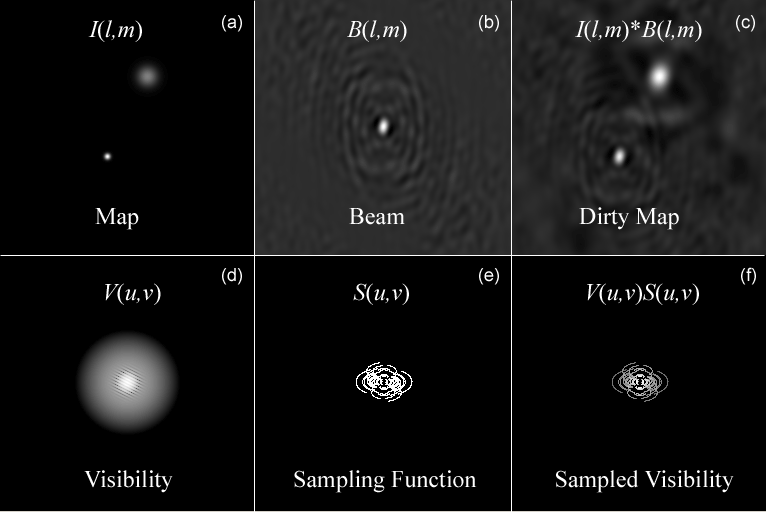
\includegraphics[width=\columnwidth]{image_ft_relation.png}
\caption[The Fourier relationship between visibilities and a radio image.]{The Fourier relationship between visibilities and a radio image. Panels along the top are the Fourier transform of panels along the bottom. Panel a shows a model sky brightness distribution, panel b is the PSF or beam of the interferometer and panel c is the dirty image. Panel d is the model visibilities of the sky, panel e is the sampling function and panel f shows the sampled visibilities.}
\label{fig:Gary}
\end{figure}
We will discuss methods for undoing this convolution shortly but first, a brief digression on the topic of beamforming with a phased array interferometer such as LOFAR.

\subsection{Phase Delays and Beamforming}
\label{sec:beamform_theory}
For steerable antennas, pointing at a phase centre is simply a matter of steering the antennas to that direction. For phased arrays such as LOFAR, and in particular the LBAs, this is unsurprisingly not possible. Instead, a time delay is digitally added to the signal from each antenna. For example, in order to maximise the response of the two element interferometer in Figure \ref{fig:2_el_int} to the direction $\hat{\Vec{s}}$, a delay of $\tau_0 = \tau_g$ must be added to the signal of antenna 2. 

\begin{figure}[ht]
    \centering
    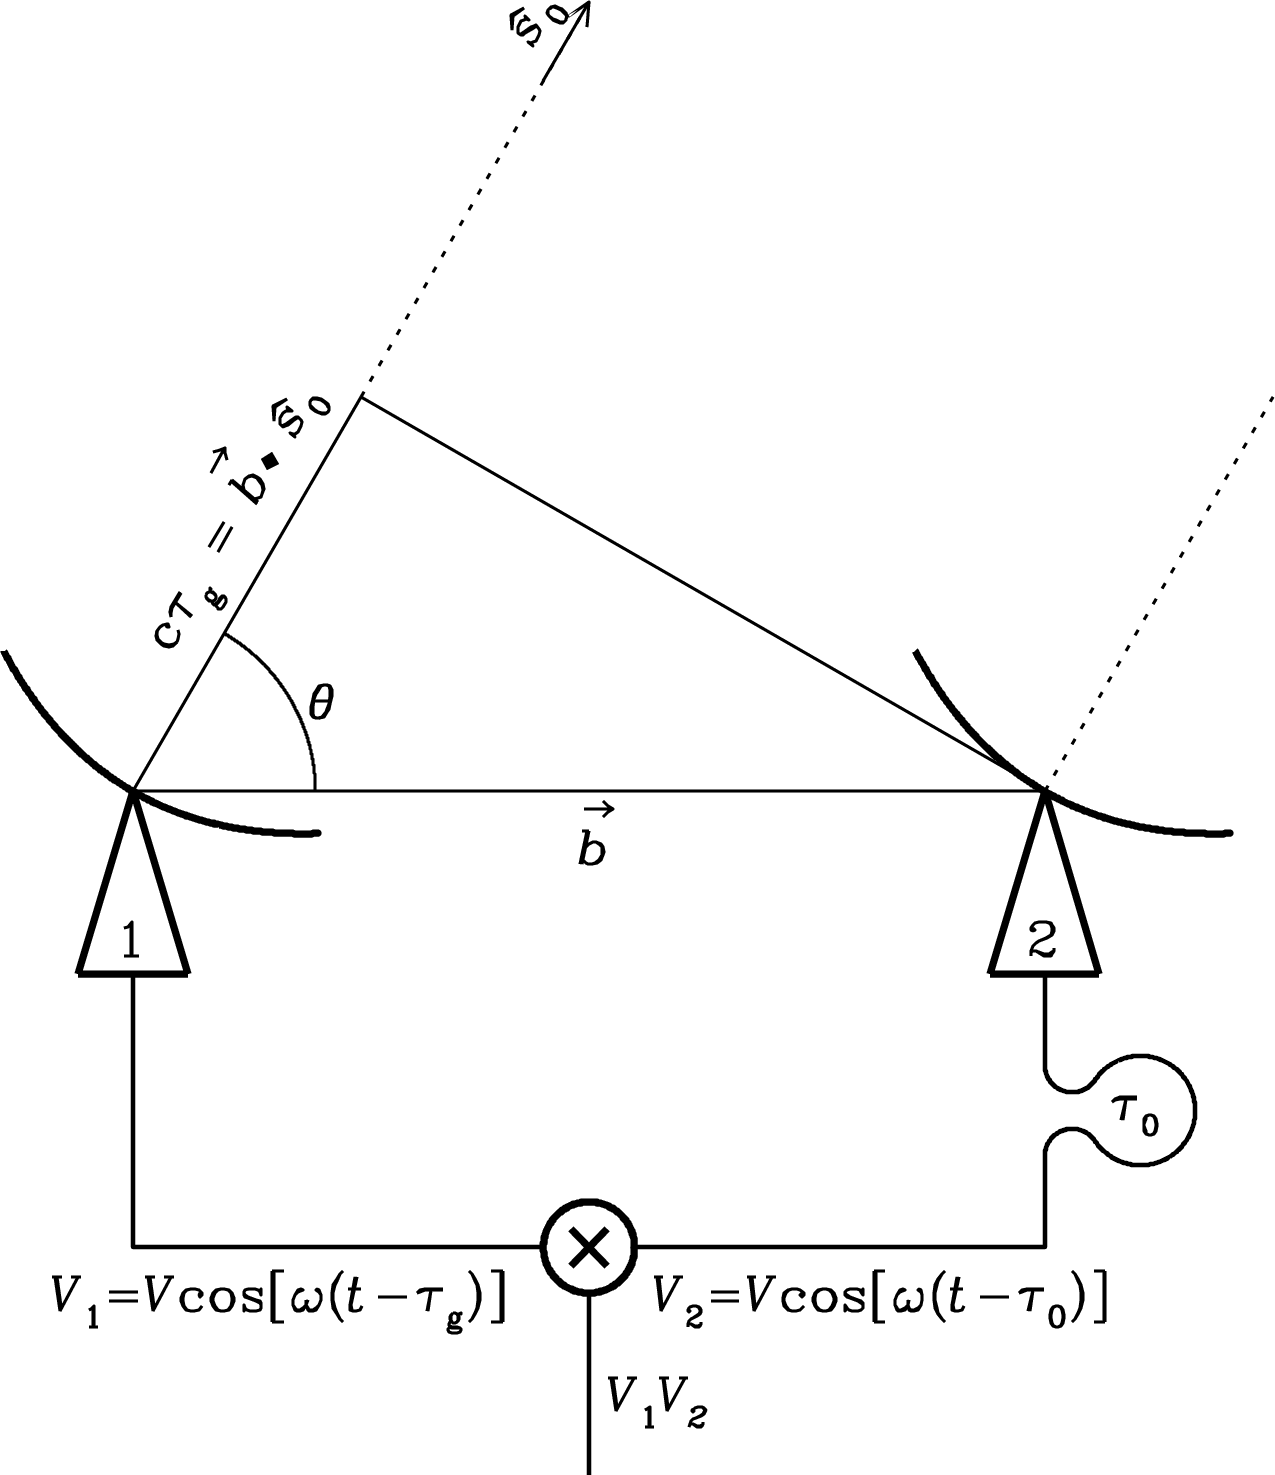
\includegraphics[width=0.75\columnwidth]{Images/2_elem_int_delay.png}
    \caption[A two element interferometer with a time delay added to one signa.]{The same interferometer from Figure \ref{fig:2_el_int}. Here a time delay of $\tau_0$ is introduced to the signal of antenna 2 by increasing the length of cable.}
    \label{fig:2_el_int_delay}
\end{figure}

Beamforming is a signal processing technique whereby all the signals are added together coherently to give a maximum sensitivity in a particular direction. The beamformed signal at the phase centre (subscript $pc$) can be described as \citep{Chen2021}
\begin{equation}
\label{eq_beamform}
F(t_{pc}) = \sum_{n=1}^N f(t_{pc} - \tau_n) w (\tau_n)
\end{equation}
for an array of N antennas. Here the a delay correction $w(\tau_n)$ is made to the signal from each antenna $f(t_{pc} - \tau_n)$ before they are summed together. The time delay $\tau_n$ has the same form as Equation \ref{eq:time_delay} for $\overrightarrow{\Vec{b}} = \mathbf{r}_n - \mathbf{r}_{pc}$. Beamforming is implemented on LOFAR in a slightly different manner. Rather than correct this delay in the time domain, the Fourier transform of the outputs of each antenna are multiplied by a phase delay $e^{- i \omega \tau}$ before being summed.
%In its most simple terms, beamforming  means pointing a phased array in a particular direction. It involves correcting for phase difference between the ``phase centre" of the beam and the position of the source of interest for each baseline and then summing it all together. 
%In order to beamform, one must account for the phase difference between the phase centre and the source (at an angular coordinate of \textit{(l,m)} with reference to the phase centre). As above, this phase difference for a baseline pq is given by, 
%$$\kappa_{pq} = 2\pi(u_{pq}l+v_{pq}m+w_{pq}(n-1))$$
%In order to correct for the phase difference and steer the beam, data for baseline pq is multiplied by the complex weight $e^{-i\kappa_{pq}}$, this is repeated for all baselines and finally all data is summed.

\subsection{Image Deconvolution}
\label{sec:imaging}
We now return to the discussion of radio interferometric imaging. Real measurements from interferometers are bound to contain some amount of noise, $\epsilon$. Thus, Equation \ref{eq:int_convolution} is more accurately written as
 
\begin{equation}
\label{eq:int_convolutionnoise}
I_\nu = I_\nu^D \ast B + \epsilon.
\end{equation}
It is for this reason that the real image cannot be obtained by simply applying the convolution theorem.  The most common method of solving this deconvolution problem is known as the CLEAN algorithm first introduced by \cite{Hogbom1974}. By assuming that true image to be made of a collection of point sources a simple iterative process over the dirty image can recreate the true image. The algorithm is outlined below:
\begin{enumerate}
\item The location and value of the brightest peak in the dirty image is found.
\item The PSF is multiplied by the intensity of this peak and what is known as the gain factor $0 < \gamma < 1$ and subtracted from the dirty image at the position of the peak.
\item The position and magnitude of the subtracted point source is recorded in a model.
\item Go to (1) unless the peak is below some predefined flux value OR a user defined number of iterations has been reached. The remaining image is now called the residual image or, simply, the residuals. 
\item Convolve the accumulated model points with an idealised PSF called the CLEAN beam. This is usually a Gaussian fitted to the main lobe of the original PSF.
\item Add the residuals to the image from (5) to form the final CLEAN image.
\end{enumerate}
You may have noticed that this is performed entirely in the image domain. This has some significant disadvantages, specifically because the PSF must be offset before subtraction, which limits how much of the image that can be deconvolved. An implementation of CLEAN in the visibility domain was developed by \cite{Clark1980} and operates in two cycles, a major and minor cycle. The major cycle starts as above by finding the position of the brightest peak. The minor cycle is then run by implementing a partial H\"ogbom clean with the threshold set to based on the first sidelobe of the PSF. The output model from the minor cycle and the PSF are both Fourier transformed and multiplied. This product is then inverse Fourier transformed and subtracted from the dirty image and the major cycle begins again. This method relies heavily on the FFT algorithm which requires the visibilities to be on a regular grid. The effect of gridding can lead to aliasing errors in the deconvolved image. 

The final implementation of the CLEAN algorithm that I will discuss, and the one that is in prevalent use in modern radio imaging software, is the Cotton-Schwab implementation from \cite{Schwab1984}. It follows the same major cycle minor cycle format as the Clark clean however the ungridded visibilities are computed for the sky model. This is done in two methods, for observations with only a few sources in the sky model, the direct Fourier transform is taken. In the more likely case of a large number of sources in the sky model, the visibilities are de-gridded after they have undergone an FFT. These model visibilities are then subtracted from the observed visibilities to produce residual visibilities. These are then imaged and the next iteration occurs.

Despite its algorithmic origins, radio imaging can be a very subjective endeavour. Not only can things like the number of iterations or gain parameter be changed to give different results, each baseline can be weighted based on their distance from the centre of the \textit{uv} plane, how many are in a given region, and everything in between \citep{Briggs1995}. As such, when trying to quantify the size of radio bursts with interferometric observations it can be undesirable to rely images that \textit{look} correct. In Chapter \ref{chap:measuring_source_sizes} I outline a technique, never before used in the context of solar radio imaging, to directly fit the visibilities and thus avoid any undesired effects from the various tweaks that can be made with imaging algorithms.
%!TEX root = ../main.tex
\doublespacing
\chapter{Measuring Source Sizes in Visibility Space}
\label{chap:wc1}

Low frequency radio wave scattering and refraction can have a dramatic effect on the observed size and position of radio sources in the solar corona.
The scattering and refraction is thought to be due to fluctuations of electron density caused by turbulence. Hence, determining the true radio source size can provide information on the turbulence in coronal plasma.
However, the lack of high spatial resolution radio interferometric observations at low frequencies such as with the LOw Frequency ARray (LOFAR) have made it difficult to determine the true radio source size and level of radio wave scattering.
Here we directly fit the visibilities of a LOFAR observation of a Type IIIb radio burst with an elliptical Gaussian to determine its source size and position. This circumvents the need for imaging of the source followed by deconvolution, which can introduce spurious effects on source size and shape.
For a burst at 34.76~MHz, we find a full width at half maximum height (FWHM) along the major and minor axes to be $18.8^\prime$~$\pm~0.1^\prime$ and $10.2^\prime$~$\pm~0.1^\prime$ respectively at a plane of sky heliocentric distance of 1.75~R$_\odot$.
Our results suggest that the level of density fluctuations in the solar corona  is  the  major  cause  of  the  scattering  of  radio  waves, resulting in  large  source  sizes. However, the magnitude of $\varepsilon$ may be smaller than previously derived in comparison to observations of radio wave scattering in tied-array images.

\section{Introduction} \label{sec:intro}
Low frequency radio wave propagation in the solar corona is not fully understood. It is widely accepted that scattering of radio waves off of density inhomogeneities plays a key role in the observed source sizes of radio bursts \citep{Fokker1965,Steinberg1971,Stewart1972,Riddle1974,Thejappa2007,Thejappa2008,Kontar2019}. However, the exact extent to which observed source sizes are broadened is difficult to measure as it requires an angular resolution to spatially resolve the source as well as an \textit{a priori} knowledge of its original size.
Current generation radio interferometers such as the LOw Frequency ARray \citep[LOFAR;][]{VanHaarlem2013b} have the resolving power to observe this angular size. This angular resolution can be exploited to accurately determine burst size and position, both of which are indicators of the level of radio scattering in the corona, which in turn is related to the level of turbulent density fluctuations. Hence a better understanding of scattering may lead to new insights into the nature of coronal turbulence.

The study of radio wave scattering in the solar corona has its origins in the 60s and 70s. \cite{Fokker1965}, \cite{Steinberg1971}, \cite{Stewart1972} and \cite{Riddle1974} did seminal work on ray tracing of radio waves in various coronal models. All concluded that sources emitted near the plasma frequency in the solar corona are enlarged due to scattering of radio waves from coronal density fluctuations. While the explanation of coronal scattering for observed source characteristics fell out of favour by the mid 1980s \citep{McLean1985}, it has seen renewed interested in low frequency radio observations in recent years  \citep{Thejappa2007,Thejappa2008,Kontar2017,Sharykin2018,Gordovskyy2019,Kontar2019}.

In low frequency imaging, the extent of scattering in the corona can be determined through the analysis of Type III radio bursts, particularly their position and size in images or decay times in dynamic spectra \citep[e.g.][]{Kontar2019, Gordovskyy2019, Krupar2018}. Given that these bursts are due to plasma emission from electron beams propagating through coronal plasma \citep[see][for a review]{Reid2014}, they provide a density diagnostic of such plasma. In particular, a subset of these bursts known as `Type IIIb' provide a diagnostic of scattering in coronal plasma due to density fluctuations from turbulence. For example, Type IIIb bursts often show fine structures or `striae' along the burst envelope \citep{Ellis1967,Ellis1969,DeLaNoe1972,DeLaNoe1975,Melnik2010b}, which are believed to be caused by density inhomogeneities in the corona \citep{Takakura1975}. Using a density model, the frequency bandwidth of these striae can be used to infer the vertical extent of the density inhomogeneity in space. A comparison of this spatial extent to observed source size in images can provide the extent to which the radio emission has been scattered \citep[e.g.][]{Kontar2017}.

Theoretically, the extent of scattering in the corona is related to the root mean squared (r.m.s) fluctuations of electron density $\varepsilon = \sqrt{\left< \delta n^2 \right>}/n$. Many recent works have assumed a value for $\varepsilon$ to use in simulations in order to recreate the time profile and source size of solar radio bursts \citep[e.g.][]{Krupar2018, Kontar2019}. However, few use the observed source size and time profile to determine $\varepsilon$. Those that have are limited to determining the value of $\varepsilon$ in the solar wind at distances $> 10 \, R_\odot$. Techniques such as interplanetary scintillations \citep[e.g.][]{Bisoi2014} and crab nebula occultation \citep{SasikumarRaja2016} have also been used to determine $\varepsilon$ at these distances. The general conclusion of these studies is that $\varepsilon$ varies slowly with heliocentric distance and has typical values of $0.001 \lesssim \varepsilon \lesssim 0.02$ in the range of 10 to 45 $\, R_\odot$. Despite this, larger values of $\varepsilon$ have been used in models. For example, \cite{Reid2010} use a value of $\varepsilon \approx 0.1$ to model electron beam transport while \cite{Kontar2019} recently used Monte Carlo simulations of scattering to determine that a value of $\varepsilon = 0.8$ is necessary in order to account for source sizes of the order of $20^\prime$, as observed by \cite{Kontar2017}. Measured values of $\varepsilon$, particularly at heights of ${\sim} 2 \, R_\odot$, are not common in the literature, with the exception of a recent study by \cite{Krupar2020}. By using observations from Parker Solar Probe \citep[PSP,][]{Fox2016}, \cite{Krupar2020} calculate a value for $\varepsilon = 0.07$ at a plasma frequency $f_p = 137$ kHz. They also find that the value of $\varepsilon$ decreases from 0.22 to 0.09 over a height range of 2.4 to 14$\, R_\odot$

It is clear that a correct interpretation of radio observations provide a means to investigate the level of scattering and density fluctuation in the corona. Advances in radio astronomy over the past 40 years have lead to increased sensitivity, temporal resolution, frequency resolution and resolving power. Modern radio telescopes such as LOFAR, the Murchison Widefield Array \citep[MWA;][]{Lonsdale2009} and the upcoming Square Kilometre Array \citep[SKA;][]{Dewdney2009} are capable of observing the predicted spatial and time profiles of Type IIIb bursts. That said, previous studies with LOFAR have tended to use tied-array imaging in this regard \citep{Kontar2017}, which has limited spatial resolution with respect to interferometric imaging.

In this paper we use LOFAR interferometric observations to determine the observed radio source size and position and how this differs from the expected source properties, which can be estimated from spectroscopy. %The discrepancy between what is observed and what is expected is used to determine the relative level of density fluctuations in the corona. 
Directly fitting interferometric visibilities provides us with the opportunity to observe low frequency radio sources at a spatial resolution in excess of what has usually been achieved. We compare our results with those of the tied-array observation from \cite{Kontar2017} and discuss the implication this may have on determining the relative level of density fluctuations in the corona. 
The remainder of this paper is outlined as follows; an observation of a Type IIIb burst is described in Section \ref{sec:obs}, in Section \ref{sec:data} we detail a method of directly fitting interferometric visibilities in order to recreate a sky brightness distribution and give results of observed source size. Section \ref{sec:data} also includes analysis of a Type IIIb stria. We conclude with a discussion in Section \ref{sec:conclusion}.

\section{Observation} \label{sec:obs}
LOFAR is an interferometric array that spans across Europe observing radio frequencies at 10 - 240 MHz. 
An interferometric observation of the Sun, utilising 36 stations (24 core and 12 remote), was performed on 17 October 2015 from 08:00 UTC to 14:00 UTC. During this time, a Type III solar radio burst was recorded  at 13:21 UTC. A calibrator source, Virgo A, was observed co-temporally in all subbands over the course of the observation.

Figure \ref{fig:context}a shows the X-ray flux measured by GOES for the duration of the LOFAR observation. A number of C-class flares can be seen in Figure \ref{fig:context}a but no significant activity is noticeable at the time of the radio burst, indicated by red vertical lines

A dynamic spectrum of the burst was recorded in the LBA band by remote station RS509 and is shown in Figure \ref{fig:context}b. The inset shows a number of striations from 34 - 35 MHz and the white cross indicates the time and frequency at which the images described in Section \ref{sec:data} are made.

The maximum baseline of the LOFAR observation is 84\,km giving sub-arcminute resolution across almost all of the observed frequency range, offering an unprecedented level of spatial resolution.

\begin{figure}
    \centering
    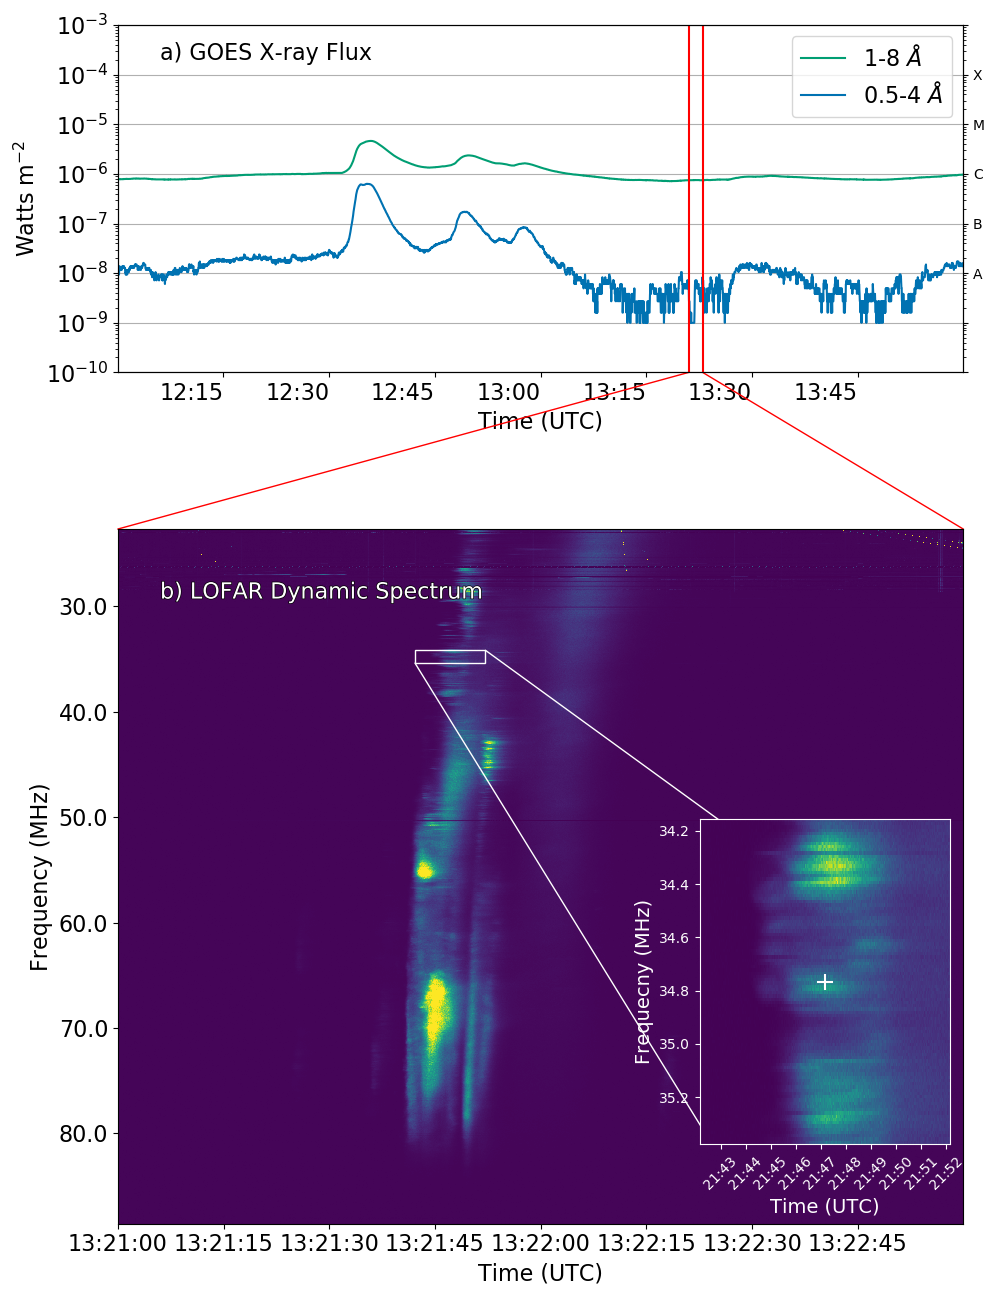
\includegraphics[width=\columnwidth]{Images/Burst_inset_goes_20200730.png}
    \caption[GOES X-ray lightcurves and dynamic spectrum for the duration of a LOFAR solar observation 2015-10-17.]{\textbf{a)} GOES X-ray lightcurves for the duration of the LOFAR solar observation. Minimal activity other than a number of C class flares prior to 13:00 UTC is observed. Red vertical lines indicate the time range of radio analysis. \textbf{b)} Dynamic spectrum of a Type III solar radio burst observed with LOFAR station RS509. We note the striations in frequency which are particularly apparent below 40 MHz. The inset is a zoom of the region in the white box showing striation in the burst. The white cross indicates the time and frequency at which the images described in Section \ref{sec:data} are made.}
    \label{fig:context}
\end{figure}

\section{Data analysis and results} \label{sec:data}
The source sizes and positions of solar radio bursts in LOFAR data have typically been obtained by the ``tied-array imaging mode" \citep{Morosan2014} whereby a number of beams are tessellated across the sun and the response in each beam is interpolated to produce an image \citep[e.g.][]{Reid2017,Kontar2017,Zucca2018, Morosan2019b}. Tied-array imaging has the distinct advantage over interferometric observations in that it retains the ${\sim} 12$ kHz frequency resolution and ${\sim} 0.01$ s temporal resolution from LOFAR beamformed observations but it also contains a significant limitation. Tied-array observations can only be made using the LOFAR core stations as they share a single clock \citep{DeGasperin2019}, which makes it possible to add beamformed data coherently. This means that the maximum baseline from tied-array observations is approximately 2 km corresponding to an angular resolution of ${\sim} 17^\prime$ at ${\sim} 30$\,MHz. Not only this, but the effect of interpolation between each tied-array beam on the observed source size has not yet been compared to observations done interferometrically. It is therefore unclear whether previously observed source sizes are in fact due to the underlying source, or an effect of the imaging technique. Solar campaigns with LOFAR are now performed with a new mode which allow for simultaneous interferometric and tied-array observations. A detailed comparison of these modes is currently under study, which should resolve the ambiguity in source sizes determined with tied-array observations (Morosan, D. E. 2020, private communication). 
%a result of this interpolation or

In order to avoid such limitations of the tied-array mode, here we use interferometric observations from the LOFAR core and remote stations, offering a longer baseline of 84\,km and hence much better spatial resolution.
The LOFAR data from this observation were calibrated using the Default Preprocessing Pipeline \cite[DPPP;][]{VanDiepen2018} and a co-temporal observation of Virgo A. This corrects for effects such as antenna band-pass, clock drift and propagation effects through the ionosphere \citep{DeGasperin2019}. We next describe our technique of directly fitting the LOFAR visibilities to estimate radio source size and position.

To produce an image from interferometric observations an inverse Fourier transform is performed on the observed visibilities, usually followed by a deconvolution of the array point spread function (PSF) from the resulting `dirty-map' of the sky-brightness distribution.
For such a deconvolution, LOFAR uses an implementation of the multi-scale CLEAN algorithm known as WSClean \citep{Offringa2014}. In this procedure a weighting may be applied to the visibilities to improve sensitivity to various spatial scales, the most common of which is the Briggs robustness weighting scheme \citep{Briggs1995}. Recreating a radio image in this way can introduce artefacts depending on the Briggs robustness used, the number of iterations of the algorithm and a number of other parameters described in more detail in \cite{Hogbom1974, Cornwell2008, Offringa2014, Offringa2017} for example. These artefacts include changes to the source shape and size. Therefore, to avoid ambiguity in the source size, shape and position due to such imaging algorithms, we directly fit the measured visibilities similar to a method used for X-ray observations using the Reuven Ramaty High Energy Solar Spectroscopic Imager \citep[RHESSI][]{Hurford2002, Kontar2010}. We describe our method in the following subsections. 

\subsection{Fitting the visibilities}
\label{sec:vis_fit}
The \textit{uv} plane is a Fourier space representation of antenna pair positions. Each point in the \textit{uv} plane is sensitive to emission of a particular angular scale. Due to the timescales over which Type III bursts occur, solar observations are limited to a sparse sample of the \textit{uv} plane and techniques to increase samples in this plane, such as aperture synthesis, cannot be used. However, the large brightness temperatures of Type III and Type IIIb radio bursts \citep{Reid2014} give rise to a  high signal to noise ratio which allows a direct fit of a model to the visibilities.
In the following we assume that the emitting source is a single elliptical Gaussian. This is based on the dynamic spectrum in Figure \ref{fig:context}b, showing the Type IIIb burst does not overlap any other bursts and as such is probably the only source in an interferometric image. The assumption leads to the convenient fact that an elliptical Gaussian in real space is observed as another elliptical Gaussian in the \textit{uv} plane. The form of this Gaussian is
\begin{equation}
V(u,v) = e^{-2\pi i(ux_0+vy_0)} \left( \frac{I_0}{2\pi} e^{-\left(\frac{\sigma_x^2(2\pi u^\prime)^2}{2}-\frac{\sigma_y^2(2\pi v^\prime)^2}{2}\right)} + C \right)
\label{eq:vis_gauss}
\end{equation}
where $x_0, y_0$ are the x and y coordinates of the source centre in real space, $\sigma_x, \sigma_y$ are the standard deviation in the x and y direction and $C$ is a constant background. Here the visibilities have been rotated to a new coordinate frame with axes $u^\prime$ and $v^\prime$ which are parallel and perpendicular to the major and minor axes of the Gaussian source such that $u^\prime = u\cos{\theta} - v\sin{\theta} \mbox{, } v^\prime = u\sin{\theta} + v\cos{\theta}$,  where $\theta$ is the angle of the major axis to the x axis, i.e. the position angle of the Gaussian on the \textit{uv} plane.

A nonlinear least squares fit is applied to the sample of visibilities in two stages. First, the source size, maximum intensity and angle relative to the x axis are found by fitting the absolute value of the complex visibilities.
In order to determine source location, the phase angle of the data is fit. Source location in real space determines fringe separation and orientation in Fourier space. The direct fitting of parameters to \textbf{$V(u,v)$} is then used to recreate the sky brightness distribution or image \textbf{$I(x,y)$}, which is the inverse Fourier Transform of Equation \ref{eq:vis_gauss}.

Figure \ref{fig:uv_fit} shows the fit of the modelled Gaussian to the complex visibilities. Due to the fact that this fit is done in Fourier space, the amplitude and phase of the data and fit are shown in the \textit{uv} plane in Figure \ref{fig:uv_fit}a and \ref{fig:uv_fit}b respectively. Here, the points are the observed visibilities and the background colour map is the fit. In Figure \ref{fig:uv_fit}a a red ellipse indicate the full width at half maximum height (FWHM) of the fitted Gaussian. The fringes in Figure~\ref{fig:uv_fit}b show the fit of the source position to the distribution of visibility phases across \textit{uv} space.
Figure \ref{fig:uv_fit}c shows the increase in the amplitude of recorded visibilities with the angular scale on the sky that causes this increase. The red curves are where data points would lie for a Gaussian in visibility space with the FWHM in the major and minor direction obtained from the fit in Figure \ref{fig:uv_fit}a.

\begin{figure}
    \centering
    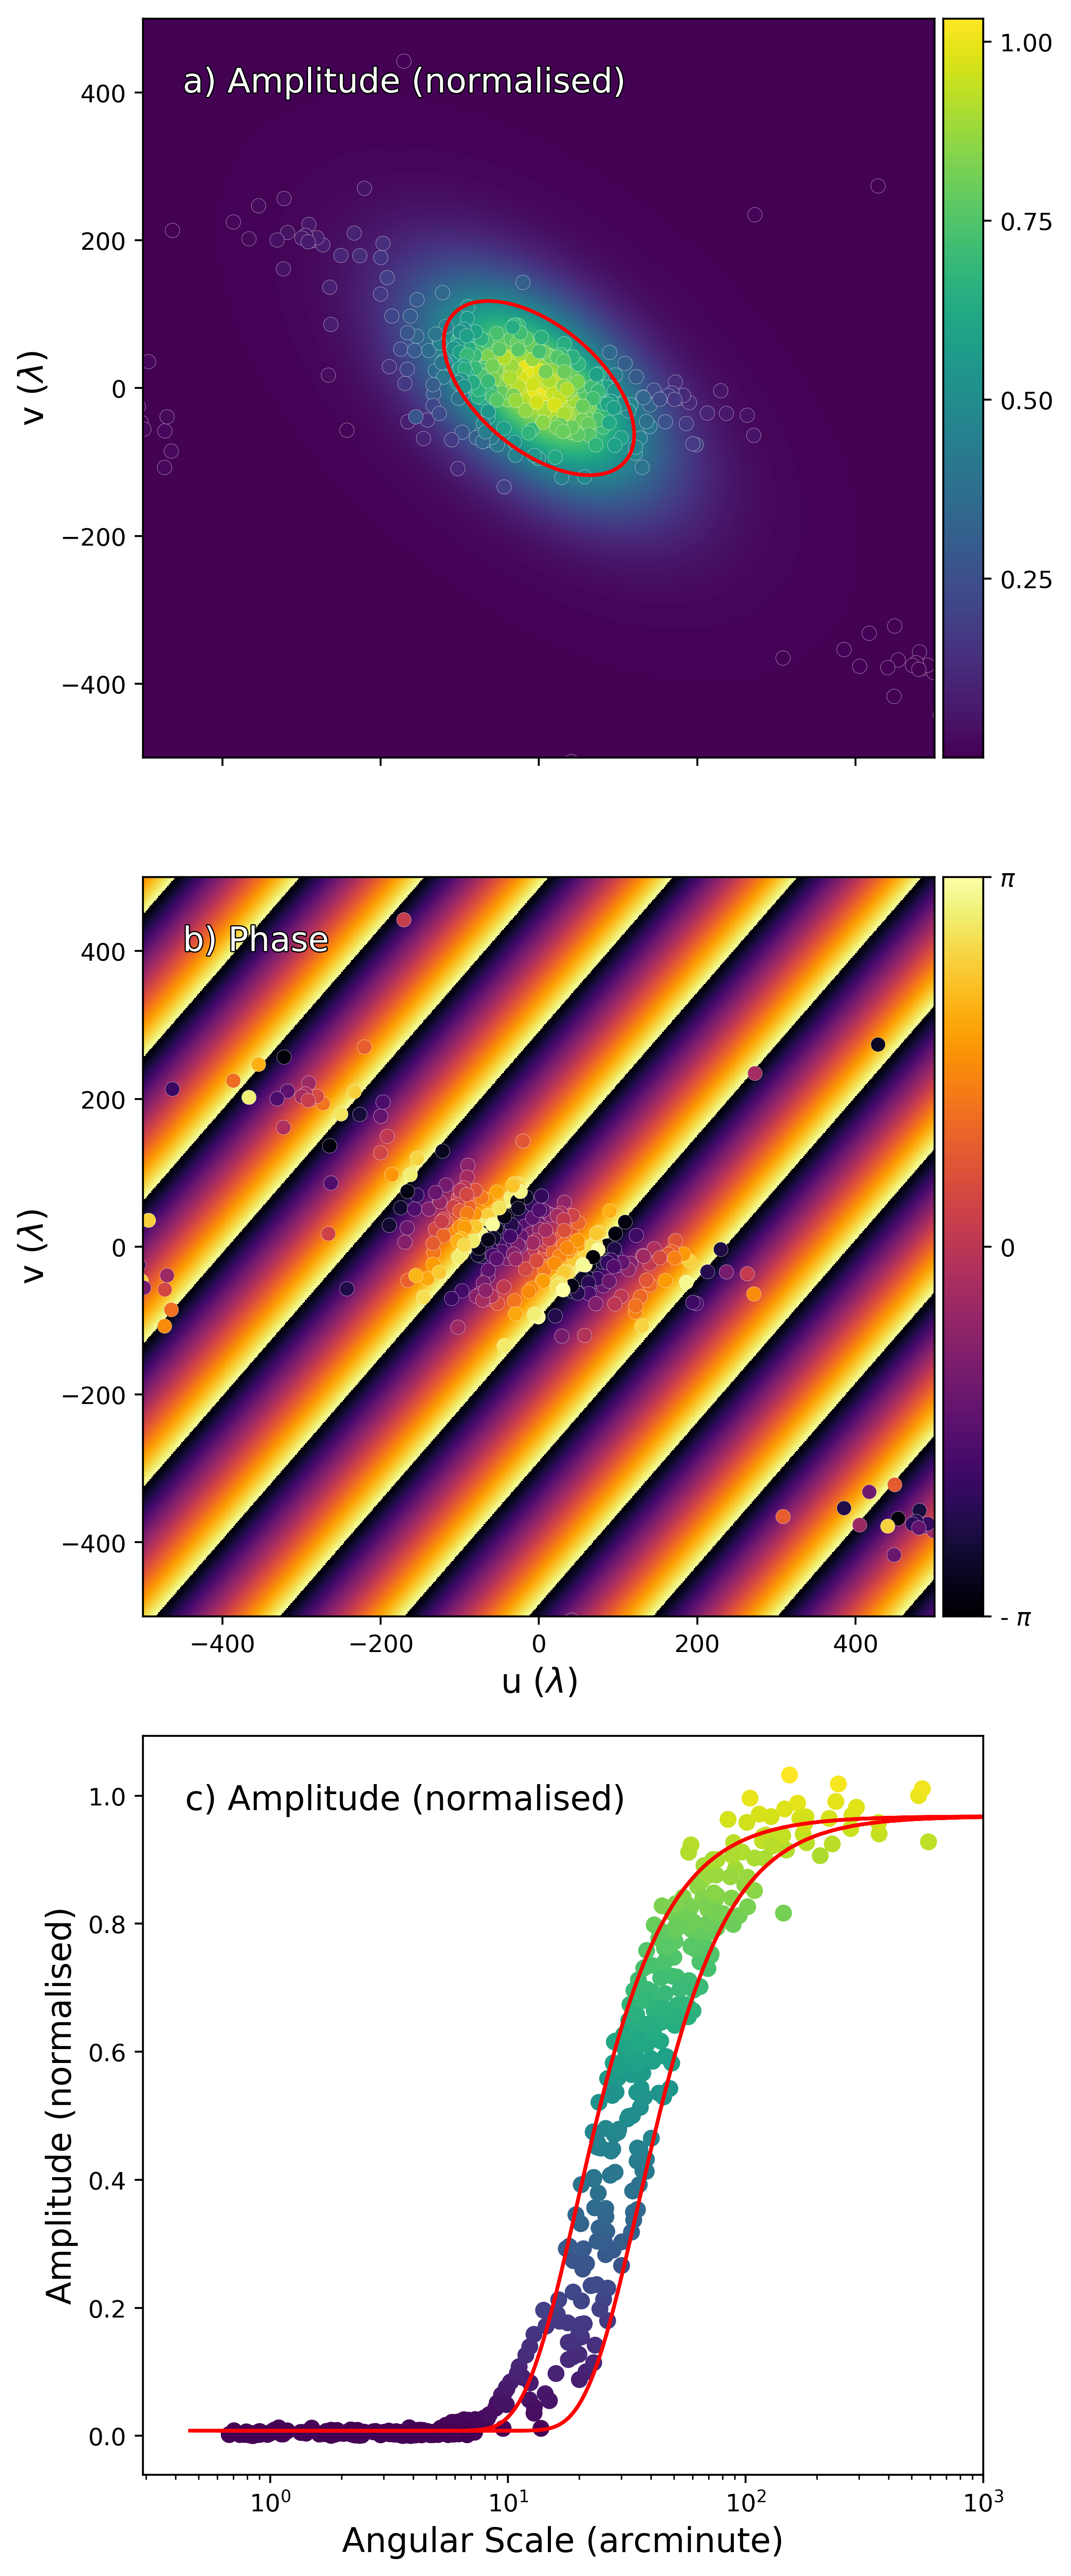
\includegraphics[width=0.5\columnwidth]{uv_fit_remote_20200826.png}
    \caption[Results of directly fitting LOFAR visibilities.]{\textbf{a)} Amplitudes of visibilities in the \textit{uv} plane for LOFAR observation. Background colour map shows a Gaussian fit. Red ellipse shows the FWHM of the normalised amplitude. \textbf{b)} Visibility phase in the \textit{uv} plane. Background colour map shows fitted phase angle. \textbf{c)} Visibility amplitudes received from different angular scales. Red curves indicate the FWHM of the semi-major and semi-minor axes of the fitted Gaussian.}
    \label{fig:uv_fit}
\end{figure}

The visibility fit reveals a source with a FWHM in real space of $18.8^\prime$ $\pm 0.1^\prime$ and $10.2^\prime$ $\pm 0.1^\prime$, in the direction of the major and minor axis, respectively. The source is found at a position of $-1312^{\prime\prime}, -1064^{\prime\prime}$ from the solar centre giving a plane of sky distance of 1.75$\, R_\odot$. The parameters from the fit can then be used to recreate a sky-brightness distribution $I(x,y)$ in real space which is shown as contours over-plotted on a 171\,\AA~ image taken by the Atmospheric Imaging Assembly \citep[AIA;][]{Lemen2012} in Figure \ref{fig:recreate}. We note that despite the theoretical high angular resolution of the long baselines afforded by LOFAR remote stations (84\,km), the source size is still large and we see little evidence of angular scales smaller than $\sim$10$^\prime$ in Figure~\ref{fig:uv_fit}c. We will discuss this further in Section \ref{sec:conclusion}.

\begin{figure}
    \centering
    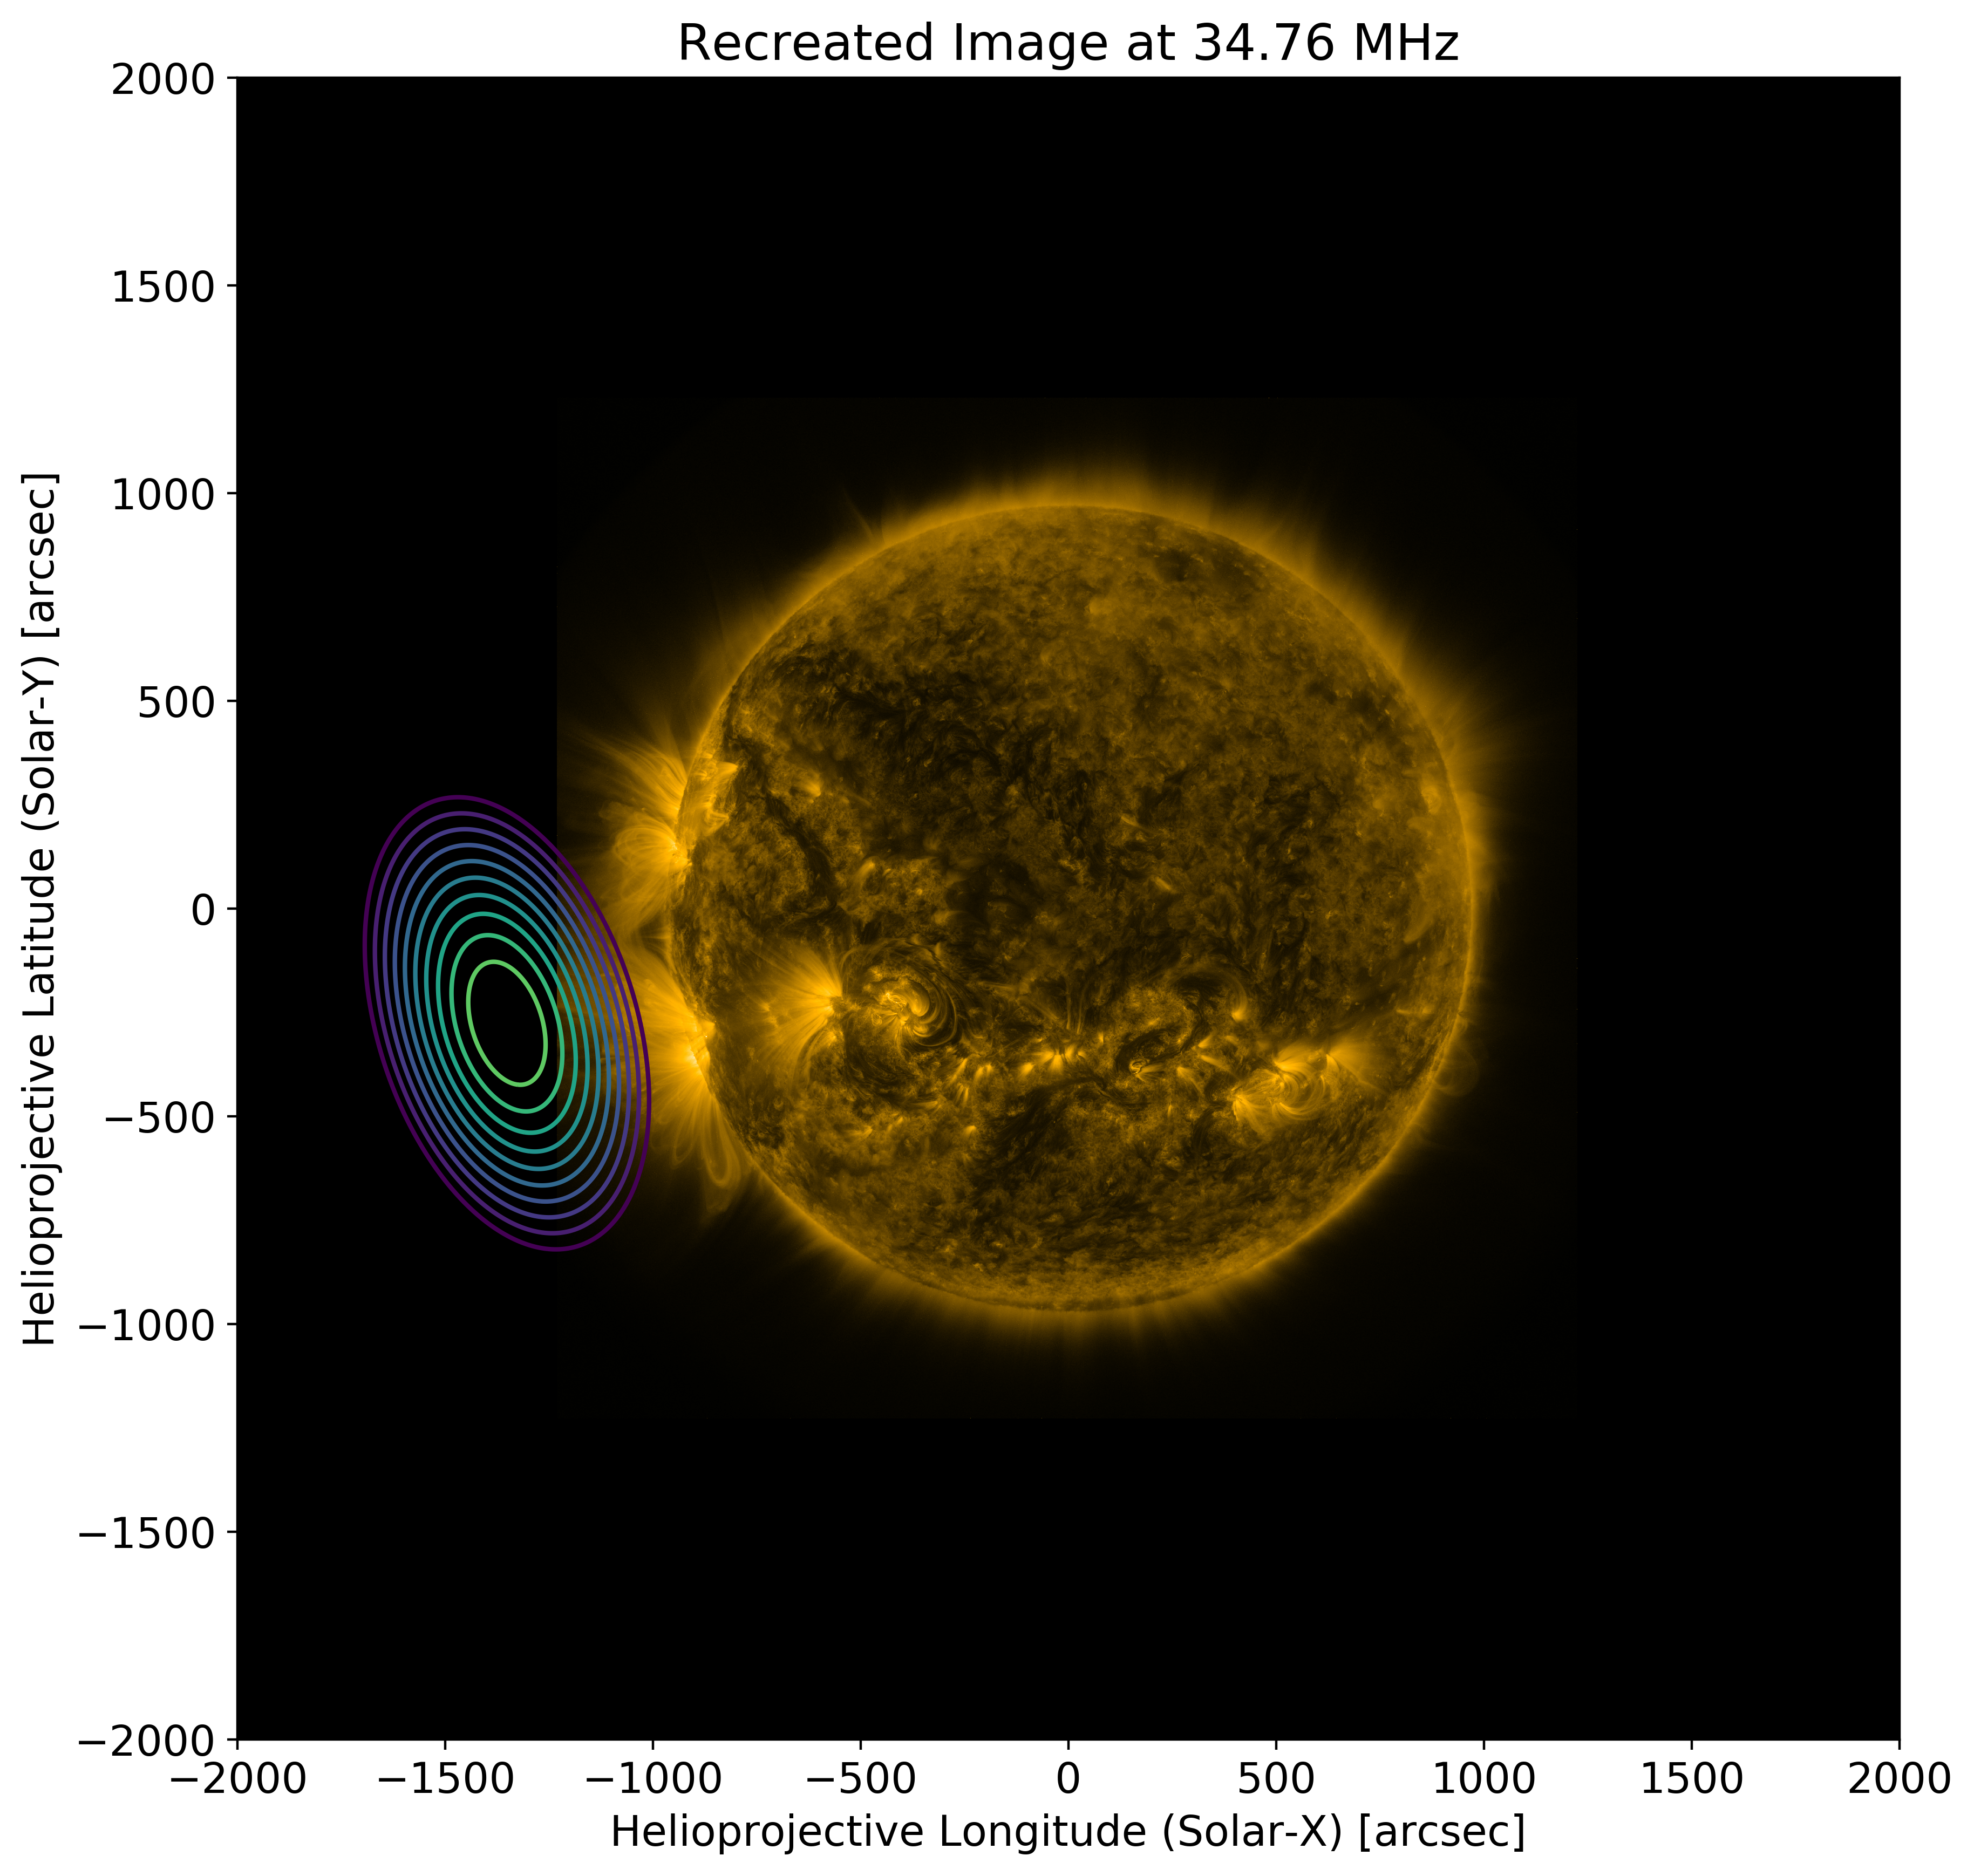
\includegraphics[width=\columnwidth]{im_recreate_remote_20200730.png}
    \caption[Recreated sky intensity profile of a Type IIIb radio burst]{Recreated sky intensity profile of a Type IIIb radio burst occurring at 13:21:46 on 17 October 2015. The background solar image is an AIA 171$\AA$ image at 17 October 2015 13:21:46 UTC.} 
    \label{fig:recreate}
\end{figure}


\subsection{Type IIIb striae}
In the above we determined the source size and position using a direct modelling of LOFAR visibility observations. This provides us with an opportunity to compare the observed source size to its actual size, which can be estimated from spectroscopic observations, similar to the method of \cite{Kontar2017}.

To estimate the source size from spectroscopic measurements, we relate the FWHM of the frequency of the striation to its vertical extent in the solar corona $\Delta r {\sim} 2L \left(\Delta f/f\right)$ where $L$ is the characteristic density scale height \citep{Kontar2017}.
A single striation was manually identified at 34.76 MHz from the dynamic spectrum. The time of maximum intensity for the burst was found and a vertical frequency slice was obtained from which $\Delta f/f$ was calculated. The individual striation, the centre of which is indicated by a white cross in the inset panel of Figure \ref{fig:context}b, was fit with a Gaussian. The value for $\Delta f$ of the striation was found from the FWHM of the fitted peak was found to be $\Delta f \sim 0.2$~MHz. The ratio of frequency to bandwidth for the striation was found to be $\Delta f/f = 0.006$, leading to an estimated source size of $3.18^{\prime\prime}$. 
Similar to \cite{Kontar2017}, this is far smaller than the source size observed from the visibility fit.

In the following section we will discuss why the most probable cause for the discrepancy in source size is radio scattering, as well as a discussion on the comparison of this observation to recent developments in the theory and the effect scattering has had on actual source size and position.

\section{Discussion}\label{sec:conclusion}

Adopting the theory described by \cite{Takakura1975} and used in \cite{Kontar2017}, the predicted source sizes of a Type IIIb striation are much smaller than what is observed. The most probable cause for this discrepancy is a combination of radio light scattering in the solar corona, propagation effects in the Earth's ionosphere and limitations due to angular resolution.
With this observation we accounted for and corrected ionospheric effects in the calibration step \citep[Section \ref{sec:data} and ][]{DeGasperin2019} thereby removing the largest uncertainty in source size and position. By fitting the source size directly in visibility space we can directly see the power at which different angular scales were observed. The \textit{uv} coverage of this observation allows angular scales of ${\sim} 42^{\prime\prime}$ to be observed (Figure \ref{fig:uv_fit}c) and although the predicted source size of ${\sim}3^{\prime\prime}$ is smaller than this, the amplitude of the observed visibilities does not increase until ${\sim} 10^\prime$ indicating that this is, in fact, the smallest source size observed in the visibilities.

It should be noted that there is better \textit{uv} coverage along one axis compared to its orthogonal which may have an effect on the eccentricity of the elliptical Gaussian fit. However, owing to the qualitatively similar shape as predicted by \cite{Kontar2019} for a burst originating near the solar limb, we are confident that the eccentricity is representative of the real source. The orientation and elongation of the source are also consistent with observations of anisotropic scattering in the solar wind \citep{Anantharamaiah1994, Ingale2015} where scattered sources are elongated perpendicular to the large scale (radial) magnetic field of the Sun.

Having accounted for all systematic effects that can affect the source size, we conclude that the large source sizes observed in this observation are due to the effect of scattering in the solar corona only. Previous tied-array observations have similar conclusions, however the tied-array technique interpolates data from a tessellation of beams across the Sun, and this introduces an ambiguity to the origin and size of sources. 
We assume the origin of the radio source to be somewhere above the active regions close to the East limb. 
An exploratory potential free source surface (PFSS) extrapolation suggests open field lines at an angle of $ \theta_s {\sim} 20^\circ$ from the plane of sky towards the observer. Similar to \cite{Chrysaphi2018} (Equations 5 and 6), we determine an out-of-plane heliocentric distance for the source. Using the observed in-plane heliocentric distance and an angle of $ \theta_s {\sim} 20^\circ$ from the plane of sky, we obtain an out-of-plane heliocentric distance of 1.82$\, R_\odot$. Comparing this to Figure 8 in \cite{Kontar2019}, which shows the effect of the angle from the plane-of-sky $\theta_s$ on source position and FWHM size in the major and minor axis, we would expect a ratio of the FWHM on the minor axis to the FWHM of the major axis to be of the order of 0.6. Our observations show a ratio of 0.54 suggesting $ \theta_s {\sim} 20^\circ$ is an appropriate approximation for the angle from the plane-of-sky.

The FWHM of the source at 34.76~MHz along the major and minor axis for this observation are $18.8^\prime$ $\pm 0.1^\prime$ and $10.2^\prime$ $\pm 0.1^\prime$ respectively. This gives the FWHM area of the source to be $A_s = 150.6~\mbox{arcmin}^2$, which we note is smaller than that of \cite{Kontar2017} who measure $A_s = 400~\mbox{arcmin}^2$ at a similar frequency of 32.5~MHz. While this could be simply due to these being two separate observations, this may be more indicative of a discrepancy between source sizes measured in interferometric observations and tied-array observations.
As mentioned in Section~\ref{sec:data}, the spatial resolution of LOFAR interferometric observations is superior to that of tied-array observations. This is mostly due to the additional stations that can be used for interferometric imaging and thus greater baseline lengths, but also due to the way tied-array images are made. Tied-array observations is carried out by pointing a number of beams in a honeycomb like pattern centred on the sun and interpolating data from each of the tessellated beams. The effect of this on observed source sizes and position is, as of yet, un-characterised. \cite{Kontar2017} attribute the large source size observed in their tied-array observation of a Type IIIb radio burst to the scattering of radio waves off of density inhomogeneities in the solar corona. It was later determined that a relative r.m.s fluctuation of electron density of $\varepsilon = 0.8$ was necessary to explain the large source size observed \cite{Kontar2019}. While it is evident that radio wave scattering causes radio bursts to appear larger in observations than predicted, the reduced spatial resolution of tied-array imaging may result in an overestimate of $\varepsilon$.

The last decade has seen a renewed interest in low frequency observations of the radio sun with state of the art radio interferometers such as LOFAR and the MWA. Radio bursts emitted via the plasma emission process give a diagnostic of the local plasma density which may give insight into the turbulent nature of coronal plasma. It is theorised that the size of low frequency radio emission is limited by scattering caused by turbulence \citep{Bastian1994}, however it is only recently that the angular resolution necessary to challenge this theory has become available. In particular, a robust comparison of sources observed with tied-array and interferometric imaging is needed. Analytical approximations of radio scattering \citep[e.g.][]{Chrysaphi2018,Gordovskyy2019,Sharma2020} have seen some success in accounting for apparent source shift and brightness temperature due to scattering, however they cannot account for the anisotropic nature of scattering and may not be appropriate to describe large angle scattering near the source location. As such, a full numerical treatment of scattering \citep[e.g.][]{Thejappa2008, Bian2019, Kontar2019}, in combination with interferometric imaging, is necessary to fully understand radio wave propagation in the turbulent coronal plasma. In order to definitively determine $\varepsilon$, more information on the power spectrum of density fluctuations and the scales on which radio scattering most effectively occurs is needed.

\section{Conclusion}
In summary, a Type IIIb radio burst was observed with LOFAR on 17 October 2015 at approximately 13:21:00 UTC. The bandwidth of an individual striation at 34.76~MHz suggests a FWHM source size of $3.18^{\prime\prime}$. Directly fitting visibilities to avoid effects of deconvolution algorithms reveals a FWHM source size in the major and minor axes of $18.8^\prime$ $\pm 0.1^\prime$ and $10.2^\prime$ $\pm 0.1^\prime$ respectively. The source is located at $-1312^{\prime\prime}, -1064^{\prime\prime}$ from the solar centre. 
Having corrected for radio wave propagation in the ionosphere, we conclude that scattering from electron density fluctuations in the solar corona is the main cause of source broadening. We discuss how values for the r.m.s relative electron density fluctuations determined from numerical models and compared to tied-array observations may be an overestimate. 
In the future, a combination of remote observations from LOFAR and \textit{in situ} measurements of plasma properties from PSP and Solar Orbiter \citep{Muller2013,Muller2020} at a variety of heliocentric distances in the corona and solar wind will be needed to form a more complete picture of coronal turbulence.
\onehalfspacing
\chapter{Scatterig Observations vs Theory}
%!TEX root = ../main.tex
\doublespacing
\chapter{Future Work and Conclusions}
\label{chap:future}
The principle goals of this thesis were to observe solar radio emission at the highest temporal, spectral and spatial resolutions to date. Firstly, the REAL-time Transient Acquisition backend (REALTA) was developed and installed at I-LOFAR to record the raw voltages from the station at $5.12 \mu$s temporal resolution. This work was published in \textit{Astronomy and Astrophysics} as \cite{Murphy2021b}
Secondly, a new technique was implemented for the first time to directly measure the size of radio bursts from their interferometric visibilities. This work was presented in Chapter \ref{chap:measuring_source_sizes} and was published in \textit{Astronomy and Astrophysics} as \cite{Murphy2021}. This technique was utilised to determine the size and shape of 29 type III bursts that were compared with predictions from state-of-the-art scattering simulations.
In this chapter I highlight some future work that could be built upon the research presented in this thesis to further advance the knowledge of radio wave generation and propagation in the solar corona. I discuss the possibility of observing radio bursts with 5~ns temporal resolution using the Transient Buffer Boards (TBBs) from I-LOFAR. Next I consider the use of machine learning algorithms to automatically detect and classify solar radio bursts recorded with I-LOFAR and REALTA. I then discuss the necessity for the development of a calibration and imaging pipeline for solar interferometry. I also outline further work that is necessary to bridge the gap between modern observations and computer simulations. This is underscored by the need for a statistical analysis of type III and type IIIb radio bursts, particular in the context of the most recent theories of spectral fine structure generation due to Langmuir wave modulation. Finally, I draw this thesis to a close with some concluding remarks.

\section{Primary Scientific Objectives}
The research that has been presented in this thesis has contributed to our knowledge of solar radio emission at low frequencies. The extent to which radio wave propagation effects distort the original shape of a radio burst has been explored. Work undertaken during this thesis has also resulted in a new facility to record and analyse radio emission using I-LOFAR. REALTA can be used to record radio observations at 5.12~$\mu$s temporal resolution. A new technique for measuring burst sizes from complex visibility data was also developed over the course of this work. Below I summarise the results from this thesis. 

\subsection{Observing Radio Bursts at the Highest Temporal Resolutions.}
The first objective of this thesis was to record the high time resolution, raw voltages from I-LOFAR to observe solar radio bursts.
In order to do this, a dedicated backend to record, store and analyse the data was necessary. Chapter \ref{chap:REALTA} outlines the development of the REALtime Transient Acquisition backend (REALTA) to serve this purpose. The seven node computer cluster receives data from I-LOFAR along a 10~Gbps fibre optic cable in four data ``lanes". After data has been recorded to disk, one of a number of processing pipelines can be run including those for solar radio observations, pulsars, FRBs, RRATs, Jovian emission and SETI. Some of the first solar radio bursts observed with I-LOFAR and REALTA are shown in Chapter \ref{chap:REALTA}. REALTA allows for high temporal resolution observations of short duration solar radio bursts such as S-bursts and can be used to analyse short duration pulsations in radio bursts. Information gained from such observations can be used to remotely determine the physics of the solar corona \citep{Morosan2015, Clarke2019} and can give insight into magnetohydrodynamic oscillations in the corona \citep{Carley2019}. This work was published in \textit{Astronomy and Astrophysics} as \cite{Murphy2021b}.

\subsection{Observing Radio Bursts at the Highest Spatial Resolutions.}
The second objective of this thesis was to determine if the size of previously observed type IIIb radio bursts was due to an effect of tied array imaging or radio wave scattering in the corona. 
This is important in determining whether or not the large source sizes of radio bursts have a physical origin or are simply due to a lack of spatial resolution. 
In Chapter \ref{chap:measuring_source_sizes} I described a new method for determining the size of a type IIIb burst directly from interferometric visibilities recorded with LOFAR. This method removes reduces the uncertainty of measured source sizes and removes any ambiguity from imaging deconvolution algorithms.
This was utilised for the first time in the context of solar observations with LOFAR to determined the size of a type IIIb burst. For a burst at 34.76~MHz, the full width at half maximum height (FWHM) along the major and minor axes was found to be 18.8~arcmin~$\pm~0.1$~arcmin and 10.2~arcmin~$\pm~0.1$~arcmin respectively at a plane of sky heliocentric distance of 1.75~R$_\odot$. The expected size of a burst at this frequency, based on the relationship between the spectral width of the striation and spatial extent of emission, was calculated to be 3.18~arcsec. The discrepancy between these two values was investigated and the results suggest that the large size observed is due to radio wave scattering. One further implication of this work is that values of $\varepsilon$ which are determined \textit{only} from tied array observations of radio bursts run the risk of over estimating the true value as the effect of imaging on source size has not been fully investigated. This work was published in \textit{Astronomy and Astrophysics} as \cite{Murphy2021}.
%the level of density fluctuations in the solar corona is the major cause of the scattering of radio waves, resulting in large source sizes. However, because of its inherently lower spatial resolution, the magnitude of $\varepsilon$ may be smaller than previously derived in comparison to observations of radio wave scattering in tied-array images. This work was published in \textit{Astronomy and Astrophysics} as \cite{Murphy2021}.

\subsection{Comparing Observations of Radio Bursts to Computational Simulations.}
The final objective of this thesis was to determine if observations of scattered sources matched the predictions of computational simulations. This was achieved by comparing a number of observations of type III bursts to simulations of radio scattering in the solar corona.
Using the new method for determining radio burst size from interferometric visibilities, the spatial properties of 29 type III radio bursts were found. The results of this analysis, comparing the similarities and discrepancies between the observations and computation scatting, are presented in Chapter \ref{chap:observations_vs_theory}.% discusses the measured similarities and discrepancies between these observations and computer simulations of scattering. 
It was found that bursts did not show the change in aspect ratio with respect to heliocentric angle as would be expected following from \cite{Kontar2019}. There are two possible explanations for this, the first being the level of anisotropy is lower than initially suggested by \cite{Kontar2019}. This is supported by an investigation of the parameter space of the scattering simulations by \cite{Zhang2021}. The other is that type III bursts have an intrinsic source size greater than the size of a point source due to scattering. This work favours the latter explanation although it is possible that both can be true. This work suggests that state-of-the-art scattering simulations still do not accurately describe all observed properties of type III radio bursts. In order to use observations of solar bursts at low radio frequencies to determine the turbulent nature of coronal plasma, these discrepancies must be rectified. This work is \textit{in prep} for a scientific publication.
 %Regardless, more must be done to align the theory and simulations with observations.
%theories of scattering are unable to account for the distribution of radio burst source sizes if they are intrinsically point sources. The more likely case is that type III radio bursts have an inherent source size larger than the size due to scattering for a point source.

\section{Future Work}
The research outlined in this thesis has furthered our knowledge of the nature of electron density fluctuations in the solar corona. Direct visibility measurements of the source size of a type IIIb burst has confirmed that density fluctuations are the main cause of large source sizes in observations and not the imaging method used. The work in this thesis has also highlighted discrepancies between observations of type III bursts and scattering simulations. Results from scattering simulations that use values of the relative root mean squared density fluctuations and degree of anisotropy in the power spectrum of fluctuations to match typical observations \citep[e.g.][]{Kontar2017} are not observed in a sample of 29 type III bursts.
%of the inherent source sizes of type III radio bursts and propagation effects due radio wave scattering. 
This work has produced a computationally and conceptually simple method to determine the size and position of a radio burst from its interferometric visibilities. Not only this but, the development of REALTA throughout this PhD allows for the recording of the raw complex voltages from I-LOFAR to study solar radio bursts. I address some open questions that remain and the possibility of future work which builds upon the research presented in this thesis below.
%First, I discuss how data from the TBBs can be utilised to produce dynamic spectra with a temporal resolution of 5~ns. Next, I describe how machine learning techniques can be used to automatically detect a radio burst in real time and how this can lower the data storage requirements of solar radio data on REALTA. I then address the need for a interferometric calibration and imaging pipeline specific to solar radio bursts. Finally, I discuss how a statistical analysis of type IIIb bursts could be useful to quantify radio wave scattering in the corona. 
%As described in \ref{chape:realta}, implementing and algorithm on REALTA to automatically determine when a radio burst has occurred will greatly simplify and reduce the data storage necessary for solar radio observations.
% in order to save on the ever growing data storage issue. Also, REALTA can be adapted to record data from I-LOFAR's TBBs which can record 5~s of data at the 200/160~MHz sampling of I-LOFAR to give the highest temporal resolution of the Sun recorded to date. 
 
\subsection{On Observing Radio Bursts with TBBs.}
One of the greatest, unexplored potentials of solar radio astronomy is extremely high temporal variability of radio bursts. The LOFAR TBBs are capable of recording 5 seconds of raw sampled data from the antennas at 5~ns temporal resolution. The TBBs are an extremely powerful tool that allow you to recreate the LOFAR data processing pipeline entirely in software. Typically, the TBB buffer is frozen before all the data is read out to an external disk. This process is much slower than the 3.2 Gbps recording of RSP data and can take upwards of 40 minutes to read out 5~s of data from every TBB. Over the period September 2017 to March 2018 a method of continually reading from the TBBs in almost real-time was investigated. I assisted in the development of this system and managed to record TBB data on a number of occasions. The data recorded during this time coincided with the solar minimum of solar cycle 24. Radio bursts occurred only once every few months and as such any data taken was essentially noise. Figure \ref{fig:TBB_timeseries} shows 10 ms of noise recorded by the TBBs from LBA number 3 at I-LOFAR.
Throughout my PhD the development of REALTA to record RSP data was a priority and as such, the possibility of a real-time readout of TBBs was not fully explored. 

%
%\begin{figure}[ht]
%\centering
%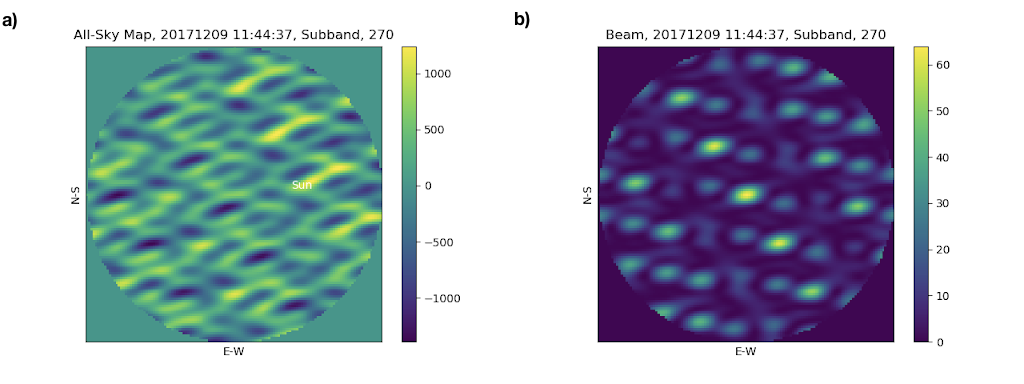
\includegraphics[width=\columnwidth]{AllSky_psf.png}
%\caption[An all sky image made with data from the TBBs at I-LOFAR]{a) An all sky image made with data from the TBBs at I-LOFAR at 52.73~MHz. b) The psf of the antennas for which TBB data was available.}
%\label{fig:TBB_allsky}
%\end{figure}
\begin{figure}[ht]
\centering
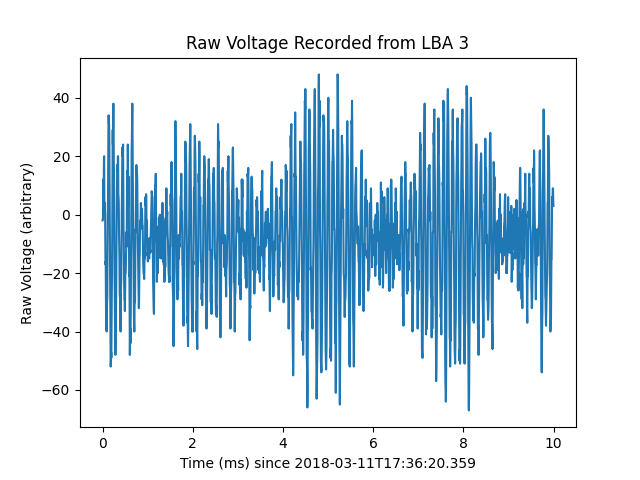
\includegraphics[width=\columnwidth]{TBBtimeseries.png}
\caption[10 ms of data recorded with TBBs from I-LOFAR.]{10 ms of data recorded with TBBs from I-LOFAR, the data presented here is from LBA 3. The beating pattern is likely due to RFI.}
\label{fig:TBB_timeseries}
\end{figure}

As was described in Section \ref{sec:sig_pipe}, TBB data is recorded before any of the digital signal processing occurs. This gives one the freedom to recreate a radio telescope entirely in software. It also allows for some unique and ingenuitive signal processing steps. For example, the polyphase filter bank in an RSP takes 1024 time samples before performing a Fourier transform to obtain 512 subbands. This results in a dynamic spectrum with a temporal resolution of 5.12~$\mu$s and 195.3~kHz spectral resolution. Using TBB data it is possible to instead, perform an FFT on the entire time series, window the resulting spectrum with any desired frequency resolution and inverse FFT each to get a dynamic spectrum with 5~ns temporal resolution and the chosen spectral resolution. 

\begin{figure}[ht]
\centering
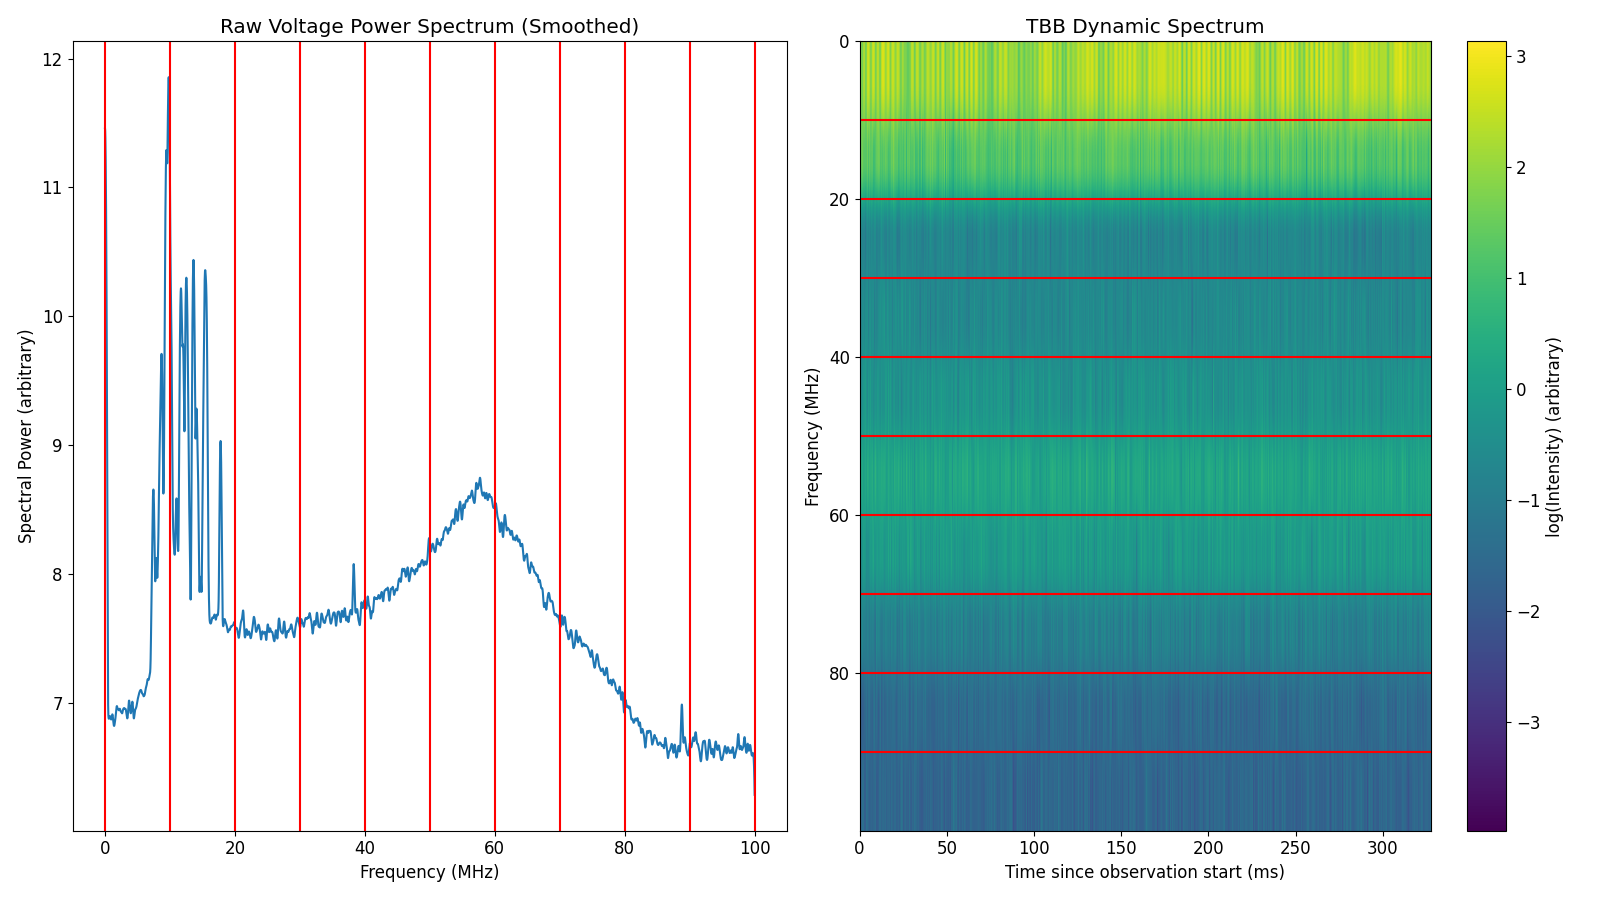
\includegraphics[width=\columnwidth]{TBB_dynamic_spectrum_power_spectrum.png}
\caption[A dynamic spectrum generated with TBB data from I-LOFAR.]{The left panel shows the (smoothed) power spectrum of an LBA. The vertical red lines mark the chosen subband edges. The right panel is a dynamic spectrum with a time resolution of 5ns and frequency resolution of $\sim 10$~MHz as determined by the chosen number of subbands, whose edges are shown by the red horizontal lines.}
\label{fig:TBB_dynamicspectrum}
\end{figure}

This is implemented on the same TBB data as shown in Figure \ref{fig:TBB_timeseries} to create the dynamic spectrum shown in Figure \ref{fig:TBB_dynamicspectrum}. The left panel shows the (smoothed) power spectrum of the time series with a number of vertical red lines which indicate the edges of chosen subbands. By performing an inverse Fourier transform on each subband, a dynamic spectrum with a temporal resolution of 5~ns can be created, shown in the right panel. Here, again, the red lines indicate the subband edges. Care must be taken to avoid spectral leakage between subbands. A common approach in avoiding this problem is to apply a window function to each subband. Because the subbands in Figure \ref{fig:TBB_dynamicspectrum} are wide and the data is mostly noise, rectangular windows are appropriate in this case.
 
The ability to record dynamic spectra and retain the 5~ns temporal resolution of the raw LOFAR sampling means that, should they exist, extremely short duration pulsations in solar radio bursts could be studied. These time scales have been completely unexplored to date and offer an exciting chance to push the forefront of solar radio astronomy. Observations at these time scales would allow for the search for fine temporal structure in radio bursts. Because the decay time of radio bursts is attributed to scattering \citep{Krupar2020}, it is likely that any inherent fine temporal structure will get ``blurred out" before being observed. However, there has been no report in scientific literature of solar radio emission at this time scale and thus any such study opens the door into the domain of nanosecond observations of the Sun.

\subsection{On the Automatic Classification of Radio Bursts.}
One of the big challenges facing radio astronomy is the vast amounts of data produced during observations. I-LOFAR produces 3.2 gigabits of data per second meaning that a 5 hour observation can reach sizes of $\sim 7$~TB. As such, observing the Sun for long durations and saving the entire raw data set regardless of whether a radio burst occurred or not is impractical. An ideal solution would be to automatically determine if a burst has occurred before choosing to save data to disk. 
This is an ideal task for a machine learning (ML) algorithm, which are most commonly used for automatic classification. ML algorithms take thousands to billions of inputs which have been labelled in order to ``learn" how to classify them. The classic example of ML automatic recognition is recognising handwritten numbers from the Modified National Institute of Standards and Technology database \citep[MNIST;][]{LeCun1998}.
\cite{Scully2021} recently showed promising results of using a particular ML algorithm, a convolutional neural network (CNN), to automatically detect and characterise type III radio bursts. They implement the YOLOv2 \citep[You Only Look Once;][]{Yolo9000} algorithm to detect type III bursts and place a bounding box that covers their time and frequency span. Figure \ref{fig:yolo} shows a dynamic spectrum with (left panel) and without (right panel) the intensity inverted and the bounding boxes detected by the CNN. Using a training dataset of simulated type III bursts, the algorithm was able to achieve and accuracy of 82.63$\%$ and can run on data in real-time.  

\begin{figure}[ht]
\centering
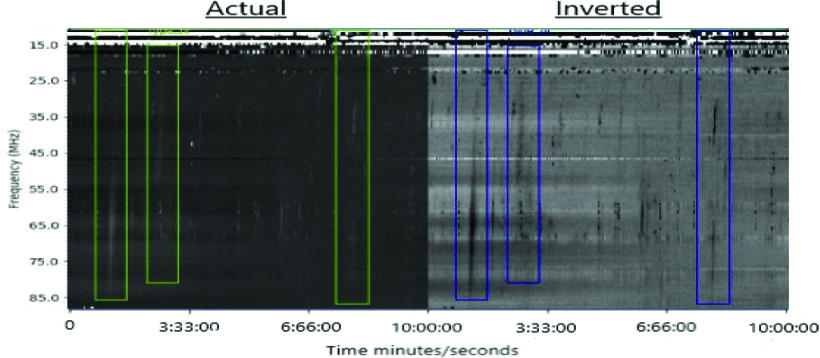
\includegraphics[width=\columnwidth]{scully_yolo.png}
\caption[Automatically detected type III bursts using YOLO.]{Automatically detected type III bursts using YOLO from \cite{Scully2021}. The colour bar has been inverted in the right panel in order to better display the type III bursts. }
\label{fig:yolo}
\end{figure}

Implementing this algorithm on REALTA and I-LOFAR would be an ideal test case on real data in real-time, especially as we enter into the next solar cycle. Not only this but, a detection from the algorithm could be used to trigger a readout of the TBBs.
In their conclusions, \cite{Scully2021} outline some future developments that could improve their results. In particular, a more physical model of type III emission is necessary, rather than the simple morphological model presently used. There is approximately 20~TB of archival data recorded with REALTA many of which contain solar radio bursts. This data, along with simulated dynamic spectra, would provide an ideal training and test set which could improve the performance of the algorithm for I-LOFAR data. The use of ML algorithms in radio data analysis will become all the more important with the next generation of radio telescopes such as the SKA which are expected to drastically increase data rates.

\subsection{On the Calibration and Interferometric Imaging of Solar Radio Bursts.}
Interferometric visibilities require calibration in order to account for the effects of the ionosphere. For LOFAR data this is performed using the Default Pre-Processing Pipeline \citep[DPPP;][]{VanDiepen2018}. An observation is made of a known calibrator source for which there is a set of model visibilities. The DPPP calibration algorithm aims to minimise the following equation
\begin{equation}
\label{eq:gain}
\vert \vert \mathbf{V}_{pq} - \mathbf{G}_p \mathbf{M}_{pq} \mathbf{G}^\dag_q \vert \vert
\end{equation}
for each baseline $pq$. Here $\mathbf{V}$ are the measured visibilities, $\mathbf{M}$ are the modelled visibilities and $\mathbf{G}$ are known as the gain matrices for each antenna $p$, $q$ and the superscript $\dag$ indicates the Hermitian conjugate. Calibration is done under the assumption of time invariability of the calibrator source. Unfortunately, if the calibrator is close enough to the Sun so that it can be seen in the sidelobes, during bursty periods such as solar radio noise storms this assumption breaks down. Calibration solutions found during these periods are inaccurate at best. The image in Figure \ref{fig:bad_cal} was made with a bad calibration solution and as such, multiple sources can be seen.

\begin{figure}[ht]
\centering
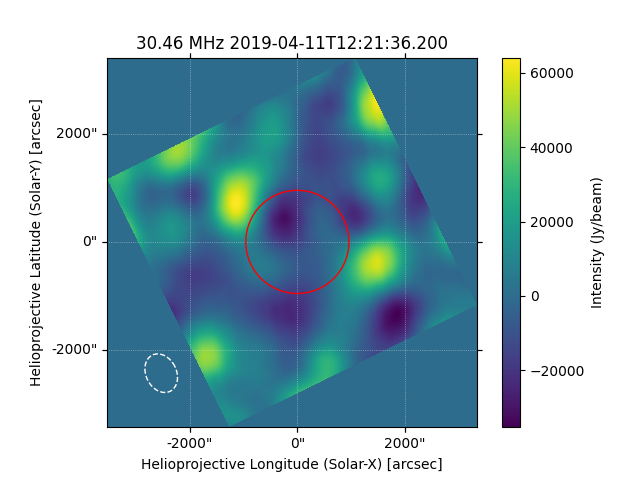
\includegraphics[width=\columnwidth]{2019-04-11T12:21:36-image.png}
\caption[An example of a solar radio burst imaged with poor calibration.]{A solar radio burst imaged with poor calibration. The colourbar shows intensity in units of Jy/beam. The red circle indicates the solar limb while the dashed white ellipse is the CLEAN beam.}
\label{fig:bad_cal}
\end{figure}

Calibration is arguably the most important step in the data processing of interferometric observations. To date, direction dependent calibration on LOFAR solar observations is not a common step taken, despite its proven success in astrophysical observations \citep{DeGasperin2019}. A method to correct for radio bursts in calibration solutions and combine this with direction dependent calibration should be developed  and self-calibration techniques developed for solar imaging with the Murchison Widefield Array \citep[MWA;][]{Mondal2019} should be implemented before the parameter space for imaging algorithms can be fully explored. 

Imaging algorithms such as CLEAN have proven themselves to be widely successful in the field of radio astronomy. However, the ability to produce different results with the same data by only changing the parameters of the algorithm is too subjective when the main focus of one's research is to determine the size of a radio burst. A number of parameters are necessary to run the CLEAN algorithm with number of iterations and weighting scheme having the most notable effect on the output image. Figure \ref{fig:briggs_comparison} shows how changing the Briggs robustness parameter for weighting the visibilites \citep{Briggs1995} affects the resulting image. The top panel shows the results for the CLEAN algorithm implemented in WSCLEAN and the bottom panel shows the results when using multiscale cleaning \citep{Offringa2017}. 

\begin{figure}[ht]
\centering
\includegraphics[width=\columnwidth]{briggs_comparison.png}
\caption[An example of the same solar radio burst imaged with different weighting parameters.]{A solar radio burst imaged multiple times changing the Briggs robustness parameter with (bottom) and without (top) multiscale cleaning.}
\label{fig:briggs_comparison}
\end{figure}

In order to consistently image the Sun it is important to determine an appropriate calibration procedure as well as standardise which parameters are to be used in imaging algorithms. Currently, there is little in the way of consensus as to how interferometric solar imaging should be done. \cite{Maguire2021} and \cite{Ryan2021} show interferometric imaging of a radio burst and the quiet radio Sun respectively using LOFAR. Their methodology is broadly similar however, was only finalised after multiple trial and error attempts. Unlike wide-field imaging or other astrophysical sources which can build upon years of research using aperture synthesis techniques, the Sun is a time dependent source and does not enjoy the legacy software that has been developed for other radio astronomy applications. 

In order to extract the most scientific value from current observations, the parameter space for the CLEAN algorithm needs to be explored to avoid making images to a subjective standard. A good start to this work would be to compare how well the algorithm can recreate a known model within the parameter space. The use of supercomputing facilities will be crucial for this to take any reasonable amount of time. 



\subsection{On the Comparisons of Type IIIb Burst Observations and Simulations.}
Type IIIb radio bursts are a subset of type III bursts that exhibit fine spectral features called striae or striations, see Section \ref{sec:typeIII}. The origin of these striations has not been conclusively determined. An early theory by \cite{Takakura1975} suggests that they are due to an electron beam passing through over dense regions in the solar corona. Recently, \cite{Reid2021} presented simulations and observations of type IIIb radio bursts where they have determined how the striae fine structure is developed. Beam driven Langmuir wave modulation by turbulence in the solar corona and the spatial motion of these Langmuir waves due to a non-zero group velocity are both necessary in order to match simulations to observed dynamic spectra and account for individual striation frequency width and duration.

%Figure \ref{fig:reid_stria} shows an individual striation for both a simulated and observed dynamic spectrum. %power density spectra for a number of type IIIb bursts with various background coronas.
%
%\begin{figure}[ht]
%\centering
%\includegraphics[width=0.5\columnwidth]{reid2021_stria.png}
%\caption[Simulated and observed type IIIb stria by \cite{Reid2021}]{Simulated and observed type IIIb stria by \cite{Reid2021}. Panel a shows an individual stria from a simulated dynamic spectrum with a background temperature of 1~MK. The black dashed line is a linear fit and gives a stria velocity of 0.6~Mm s$^{-1}$ whereas the red dashed line is a quadratic fit with an initial velocity of 0.63~Mm s$^{-1}$ and a final velocity of 0.76~Mm s$^{-1}$. Panel b shows an individual stria from the type IIIb burst on 16 April 2015. The black dashed line is a linear fit with a velocity of 0.69~Mm s$^{-1}$.}
%\label{fig:reid_stria}
%\end{figure}
%
%\begin{figure}[ht]
%\centering
%\includegraphics[width=0.75\columnwidth]{reid2021_powerdensityspectra.png}
%\caption[Power density spectrum of observed and simulated type IIIb bursts by \cite{Reid2021}]{Power density spectrum of observed and simulated type IIIb bursts by \cite{Reid2021}. Panel a shows power density spectra for type IIIb bursts observed with LOFAR on 16 September 2015 (red), 16 April 2015 (blue) and 24 June 2015 (green). Panel b shows the power density spectra for simulated type IIIb bursts with a background corona temperature of 1 MK (blue), 10 MK (red) and without a group velocity (green). The dashed balck lines indicate a power law of -5/3, consistent with a Kolmogorov description of turbulence.}
%\label{fig:reid_pds}
%\end{figure}
Following the results from this thesis, the effect radio wave scattering has on the size of type III bursts does not fully agree with scattering simulations (Chapter \ref{chap:observations_vs_theory}). As such, more work is necessary to determine the probable causes of this discrepancy. One possible avenue of investigation would be to perform a similar analysis to Chapter \ref{chap:observations_vs_theory} for type IIIb bursts. By using Equation 1 in \cite{Reid2021}, it would be possible to obtain a value of $\varepsilon$ directly from the dynamic spectrum of a type IIIb burst. Coupling this together with the burst size would give a more qualitative comparison to scattering simulations than has been done previously. Figure \ref{fig:reid_peakflux} shows the peak flux of an observed type IIIb burst on 16 September 2015. The green curve shows the smoothed flux which is used to determine $\Delta I/I$ in Equation 1 of \cite{Reid2021} and hence determines a value for $\varepsilon$.

\begin{figure}[ht]
\centering
\includegraphics[width=0.75\columnwidth]{reid2021_peak_flux.png}
\caption[Peak flux of a type IIIb burst observed by \cite{Reid2021}.]{Peak flux of a type IIIb burst observed by \cite{Reid2021} on 16 September 2015. The green curve shows the smoothed flux which is used to calculate $\Delta I/I$ from their Equation 1.}
\label{fig:reid_peakflux}
\end{figure}

A previous case study of a type IIIb - III pair (a fundamental-harmonic pair of type III bursts where the fundamental is a type IIIb and the harmonic a type III) was carried out by \cite{Zhang2020}. They found that the fundamental and harmonic emission show different motion as can be seen in Figure \ref{fig:typeIIIbIII} and attribute this to radio wave propagation effects.

\begin{figure}[ht]
\centering
\includegraphics[width=0.7\columnwidth]{Zhang_2020.png}
\caption[Type IIIb - III pair observed by \cite{Zhang2020}.]{A type IIIb - III pair observed by \cite{Zhang2020}. Panels a1-3 show the fundamental type IIIb burst observed with LOFAR and imaged using WSCLEAN. Panels b1-6 show the harmonic type III burst at a frequency of 26.56~MHz.}
\label{fig:typeIIIbIII}
\end{figure}

To date there has been no comparison between a large number of type III and type IIIb bursts where both are emitting at the fundamental plasma frequency using interferometric observations. Applying a technique similar to the visibility fitting described elsewhere in this thesis to determine a characteristic size could be extremely useful in quantifying the level of turbulence necessary to generate type IIIb bursts. This is also an excellent opportunity to use \textit{in-situ} data from Parker Solar Probe \citep[PSP;][]{Fox2016} and Solar Orbiter \citep{Muller2020} to confirm the predictions made with remote measurements from LOFAR and other radio telescopes. 

%\subsection{On the Structure Function of Density Turbulence in the Corona.}
%\cite{Bastian1994} describes the

\section{Concluding Remarks.}
The research presented in this thesis is a study of the low radio frequency Sun at some of the highest temporal, spectral and spatial resolutions to date. Our knowledge of radio wave propagation in the solar corona has been expanded as a result and the potential for further study is great. Using a new method in the context of LOFAR solar observations that I developed, I determined that the large size observed for a type IIIb radio burst is due to radio wave scattering in the corona and that this effect may be over estimated by previous tied array imaging observations of the same. Following from this, I investigated the source size and position of 29 type III bursts using the same method. My conclusion from this is that the level of anisotropy of radio wave scattering is lower than first expected by simulations and that type III bursts have an intrinsic source size of the order of 10 arcmins. Parallel to this, I helped develop and install REALTA at I-LOFAR which has recorded numerous radio noise storms at 5.12~$\mu$s temporal resolution and 195.3~kHz spectral resolution. 

With the upgrade to LOFAR2.0 and other next generation radio telescopes such as the Square Kilometre Array \citep[SKA;][]{McMullin2020} imminent, automatic detection of solar radio bursts will become all the more important. Machine learning algorithms have an important part to play in the automatic detection and classification of solar radio bursts in the near future. Until then, development of solar specific calibration and imaging techniques can help maximise the quality of observations from modern day interferometers such as LOFAR.  

There are many questions that remain unanswered about radio wave scattering in the corona, the most relevant to this thesis being why do scattering models not fully agree with observations? Recent advancements in the theory of fine structure generation in type IIIb bursts may bridge the gap between observations and simulations.

The work and research undertaken as part of this thesis has improved our understanding of and ability to observe and analyse solar radio emission. By combining the imaging technique developed during this thesis with \textit{in-situ} measurements of coronal plasma, some of the long standing questions in radio wave propagation are bound to be answered. 
%They say science is done incrementally. In that case, this thesis is as incremental as it gets. While I do not claim to have made any ground breaking discoveries, I do truly believe that the work and research undertaken as part of this thesis has improved our understanding of and ability to observe and analyse solar radio emission. I have but marked the path, it is for others to now follow it.	
















% --------------------------------------------------------------
%:                  BACK MATTER: appendices, refs,..
% --------------------------------------------------------------

%: ----------------------- bibliography ------------------------

\newgeometry{left=1.6cm, right=1.6cm, top=-2.0cm, bottom=1.0cm, footskip=0cm}
\singlespacing
\begin{footnotesize} 
\bibliographystyle{natbib}
\renewcommand{\bibname}{References} 
%\begin{multicols}{2}

\bibliography{thesis_references}

%\end{multicols}

\singlespacing
\end{footnotesize}
\restoregeometry

\appendix
%%!TEX root = ../main.tex
%Adding the above line, with the name of your base .tex file (in this case "thesis.tex") will allow you to compile the whole thesis even when working inside one of the chapter tex files

% \chapter{TBB Software}
% \label{app:TBB_software}
% In order to create dynamic spectra from TBB data, the channelisation of a LOFAR RSP board must be replicated. For brevity's sake, the following discussion will ignore the procedure to beamform as it is simply an implementation of the theory described in section \ref{sec:beamform_theory}. 

% In order to preserve the 5 ns time resolution of TBB data the raw voltage data must first undergo a Fourier transform. This can be though of as representing the entire signal time series as power per frequency with frequency resolution governed by the relation from a discrete Fourier transform (DFT),
% $$\Delta f = \frac{1}{N\Delta t}$$
% where $\Delta f$ is the frequency resolution, $N$ is the number of points the DFT uses and $\Delta t$ is the time resolution. Depending on the desired frequency resolution, the data spectrum obtained from the DFT is then split into a number of ``subbands" which are analogous to subbands produced in an RSP board (Figure \ref{fig:subbands_pspec}). One subband is selected while the rest of the spectrum is set to zero so that an inverse DFT can be performed resulting in the initial 5 ns time resolution. This is done for each subband so that a number of time series at a particular frequency range. These time series are then stacked and represented as a dynamic spectrum such as the one in Figure \ref{fig:TBB_dspec}.

% \begin{figure}
%     \centering
%     \includegraphics[width=0.75\columnwidth]{Images/p_spec_smooth.png}
%     \caption[Spectrum of TBB data and subbands]{A sample spectrum of TBB data. The spectrum is smoothed for clarity and the subband edges are shown as red vertical lines.}
%     \label{fig:subbands_pspec}
% \end{figure}

% \begin{figure}
%     \centering
%     \includegraphics[width=0.75\columnwidth]{Images/TBB_dynamic_spectrum.png}
%     \caption[Dynamic spectrum of TBB data]{The dynamic spectrum by channelising in the method outlined above.}
%     \label{fig:TBB_dspec}
% \end{figure}

% Performing channelisation in this way gives a user the freedom to select any frequency range to channelise within the band with any frequency resolution. There are however, a few undesired effects of too fine a frequency resolution. Firstly, windowing a DFT produces unwanted sidelobes in the reconstructed time series and also serves to broaden sharp peaks. Before further work can be done using this code, the effects of different DFT window sizes must be characterised.
%  %There is one major distinction between the channelisation in an RSP and in software.

\chapter{Plasma Emission}
\label{app:plasma}
In 1942 while Britain was on the look out for radar signals of enemy aircraft, a strong, noise like and highly variable signal was noticed by radar operators. Initially it was thought that Germany had managed to learn the secret of radar and create some sort of jamming device. On further investigation it was found that this jamming was in fact radio emission from the Sun. The discovery of this radio emission being associated with a major solar flare was kept secret until after the war and was published by \cite{Appleton1946}.
Since then a number of major advancements in both instrumentation and theory have occurred. A culmination of the theory of solar radio emission is laid out in the book by \cite{McLean1985} while worldwide, a number of extraordinary radio telescopes and interferometers such as the LOw Frequency ARray (LOFAR, \citeauthor{VanHaarlem2013b} \citeyear{VanHaarlem2013b}), the Nan\c{c}ay Radio Heliograph and the Murchison Widefield Array (MWA), to name but a few, have been built.

Solar radio emission often comes in the form of bursts of varying timescales. These were initially classified into three types by \cite{Wild1950b} with a fourth and fifth type being discovered by \cite{Boischot1957} and \cite{Wild1959} respectively. Of these, the most frequently occurring are the so called Type III radio bursts. These are short bursts that can be observed over many frequencies and are found to be associated with solar flares \citep{Malville1962}. An initial study into how they are emitted was conducted by \cite{Ginzburg1958}.% This essay examines Type III bursts and in particular describes their observed characteristics, what causes them and the plasma emission process of their generation.

%\section{Process of Forming Type III Bursts} %(This is how they're made)}
For a Type III radio burst to be emitted, an electron must generate Langmuir waves in the plasma. These Langmuir waves then go on to generate electromagnetic transverse waves by coalescing with other waves or by decaying. Theses electromagnetic waves are the radio bursts that are observed. In this section the generation of Langmuir waves and the process of plasma emission are discussed.

\section{Generation of Langmuir Waves}
During magnetic reconnection in a solar flare electrons are accelerated along magnetic field lines. As these beams of electrons propagate, faster electrons begin to outpace slower electrons and stationary ions in the background plasma. This leads to a second peak on the Maxwell Boltzmann distribution of velocities as seen in Figure \ref{fig:Lwavegrowth}. Energy is transferred from electrons electrons travelling at the phase velocity, $v_{\phi}$ , to Langmuir waves creating a resonance.
The positive velocity gradient of this resonance means that there are more electrons with velocity greater than $v_{\phi}$ than there are electrons with velocities less than  $v_{\phi}$ (where energy is transferred from the wave to the particles), this causes Langmuir waves to become unstable and their magnitudes to grow exponentially. Particles with velocities near $v_{\phi}$ are in resonance with the Langmuir waves and drive this instability.

This instability is alleviated by what is known as quasi-linear relaxation \citep{Melrose1987} whereby the resonant behaviour of the electrons and Langmuir waves results in a plateau in the Maxwell Boltzmann distribution rather than a second peak. It can be shown that \citep{Vedenov1963} the electron distribution function, $f(v,t)$ where $\int f(v,t) dv = n_e$, and the spectral energy index of Langmuir waves, $W(v,t)$ such that $\int W(v,t) dv = E_L$ the total energy density, can be expressed as follows \citep{Reid2014},
\begin{equation}\label{eq:dfdt}
    \frac{\partial f(v,t)}{\partial t}=\frac{4 \pi^2 e^2}{m_e^2} \frac{\partial}{\partial v} \left( \frac{W}{v} \right) \frac{\partial f(v,t)}{\partial v}
\end{equation}

\begin{equation}\label{eq:dWdt}
    \frac{\partial W(v,t)}{\partial t}= \frac{\pi \omega_p}{n_e} v^2 W \frac{\partial f(v,t)}{\partial v}
\end{equation}

Equation \ref{eq:dWdt} shows that the growth rate of Langmuir waves is proportional to $\frac{\partial f(v,t)}{\partial v}$, hence a positive gradient in the Maxwell Boltzmann distribution leads to a growth in Langmuir waves. The right hand side of Eq. \ref{eq:dfdt} has a diffusion operator $D=\frac{W}{v}$. This states that the transfer of energy from particles to waves and back leads to the distribution function being smoothed out and eventually becoming a plateau. The evolution of $f(v,t)$ and $W(v,t)$ with time is shown in Figure \ref{fig:Lwavegrowth}. Figure \ref{fig:Lwavegrowth} shows how the plateau in the distribution function and a broadening in the spectral energy density develop as time progresses.

\begin{figure}
    \centering
    \includegraphics[width=0.75\columnwidth]{Images/L_wave_growth.png}
    \caption[Langmuir wave distriburtion function and spectral energy density.]{Left: Evolution of distribution function (normalised by the electron thermal velocity $v_{Te}=V_e$) in time. The diffusive term in \ref{eq:dfdt} causes the bump-on-tail Gaussian to turn into a plateau, thereby eliminating the instability caused by the positive velocity gradient. Right: The spectral energy density of generated Langmuir waves, x-axis normalised to the Debye length $\lambda_D=\sqrt{\frac{\epsilon_0 k_B T_e}{e^2 n_e}}$. As time passes the spectral range of Langmuir waves increases. Each panel shows successive times of t=0.15s (green, dot-dashed line) and t=2.50s (red, dotted line). \citep[Figure taken from][]{Reid2014}.} %(Figure taken from \citeauthor{Reid2014} \citeyear{Reid2014})}
    \label{fig:Lwavegrowth}
\end{figure}

\section{Wave-Wave Interaction}\label{Plasma Emission}
Wave-wave interaction concerns the processes by which three types of waves interact. These are: transverse (T) waves, Langmuir (L) waves and ion sound (S) waves, and have the following, respective dispersion relations,
$$ \omega=(\omega_p^2 +k^2c^2)^{\frac{1}{2}} $$
$$ \omega \cong \omega_p + \frac{3k^2V_e^2}{2 \omega_p}$$
$$ \omega = kv_s $$
where $V_e$ is the thermal velocity of electrons in the plasma, $v_s$ is the ion sound speed and $k$ is the wave vector. Only transverse waves with $\omega > \omega_p $ can escape and thus a plasma emission mechanism is a process that generates these transverse waves. 

As mentioned in Section \ref{characteristics}, Type III bursts have a harmonic structure associated with plasma emission at the plasma frequency and the second harmonic. Both of these transverse waves are formed in different three wave processes that will now be discussed.
In a plasma, due to scattering from other wave modes and ions in the plasma, a wave mode can be changed from one to the other. This is expressed in the equation 
$$ \sigma \rightleftarrows \sigma' + \sigma '' $$
where $\sigma$, $\sigma'$  and  $\sigma ''$ represent different wave modes. Conservation of energy and momentum state,
$$ \omega^{\sigma}(k)=\omega^{\sigma'}(k')+\omega^{\sigma''}(k'')$$
$$ k=k'+k''$$
where $ \omega^{\sigma}(k)$ is the frequency of a particular wave mode with the wave vector $k$. For Langmuir (L), ion sound (S) and transverse (T) wave modes the allowed processes are L+S$\rightarrow$L', L+S$\rightarrow$T,  T+S$\rightarrow$L,  T+S$\rightarrow$T' and  L+L'$\rightarrow$T. Of these L+S$\rightarrow$T,  L$\rightarrow$T+S are responsible for fundamental emission while harmonic emission is associated with the three wave process L+L'$\rightarrow$T.

Originally \cite{Ginzburg1958} considered fundamental emission to be due to Langmuir waves scattering off of thermal ions in the plasma. It is now commonly accepted that the biggest cause of fundamental emission is due to the three wave processes of a Langmuir wave coalescing with an ion sound wave generated by L$\rightarrow$L'+S or when a Langmuir wave decays into an ion sound wave and an electromagnetic transverse wave. The process L$\rightarrow$T+S can be visualised as in Figure \ref{fig:Femission}. In solar radio physics it is often assumed that $k_L \gg k_T$, knowing this and that the wave vectors must satisfy $\mathbf{k}_L \pm \mathbf{k}_s = \mathbf{k}_T$ ($+$ for L+S$\rightarrow$T , $-$ for L$\rightarrow$T+S) implies $\mathbf{k}_s \approx \mp \mathbf{k}_L$ 

\begin{figure}
\centering
\includegraphics[width=0.5\columnwidth]{Images/Fundamental_emission_Lwaves.png}
\caption[A three wave process of fundamental plasma emission L$\rightarrow$T+S]{A three wave process of fundamental plasma emission L$\rightarrow$T+S. A Langmuir wave decaying into an ion sound wave and an electromagnetic transverse wave at the plasma frequency. (Figure adapted from Solar (interplanetary) Radio Bursts: the Generation of Radio Waves,	an oral presentation by David Malaspina at the Jean Louis Steinberg International Workshop on Solar, Heliospheric and Magnetospheric Radioastronomy, November 2017)}
\label{fig:Femission}
\end{figure}

Second harmonic emission occurs when two Langmuir waves coalesce in the process L+L'$\rightarrow$=T, shown in Figure \ref{fig:Hemission}. Conservation of momentum requires that $\mathbf{k}_L + \mathbf{k'}_L = \mathbf{k}_T$ and for second harmonic (H) generation, $k_T=k_H \approx \frac{\sqrt{3} \omega_p}{c}$. The phase speed $v_\phi$ of Langmuir waves is much less than $\frac{c}{\sqrt{3}}$ meaning that $k_L \gg k_T$ which results in $\mathbf{k}_L \approx -\mathbf{k'}_L$. This means that for a transverse wave at the second harmonic to be created, two Langmuir waves must coalesce almost exactly head on. These backward propagating Langmuir waves are generated: in the three wave processes of L+S$\rightarrow$L' and L$\rightarrow$L'+S; scattering off of thermal ions; and refraction at density inhomogeneities.
 \begin{figure}

     \centering
     \includegraphics[width=0.5\columnwidth]{Images/Harmonic_emission_Lwaves.png}
     \caption[Three wave process of second harmonic plasma emission L+L' $\rightarrow$ T]{Three wave process of second harmonic plasma emission L+L' $\rightarrow$ T. A Langmuir wave (L) and a backwards propagating Langmuir wave (L') coalesce to form a transverse wave (T) at $2 \omega_p$. (Figure adapted from Solar (interplanetary) Radio Bursts: the Generation of Radio Waves,	an oral presentation by David Malaspina at the Jean Louis Steinberg International Workshop on Solar, Heliospheric and Magnetospheric Radioastronomy, November 2017)}
     \label{fig:Hemission}
 \end{figure}
 
\chapter{2017-10-15 Type III Burst}
\label{app:event}
The Type III burst which occurred at 13:21 UTC is shown in the composite radio spectra in Figure \ref{fig:comp_spec} and was not co-temporal with any other solar event.
EUV images of the Sun such as those taken in the 193{\AA} channel with AIA, Figure \ref{fig:AIA_GOES}a, show a number of bright active regions and a coronal hole which give indications of where to expect closed and open magnetic field lines.
Xray flux around the time of the Type III burst was measured by the Geostationary Operational Environmental Satellite (GOES, seen in Figure \ref{fig:AIA_GOES}b). It should be noted that there were a number of small C class solar flares before the radio burst however none were co-temporal. 
\newline
\begin{figure}[h]
    \centering
    \includegraphics[width=0.75\columnwidth]{Images/aia_goes.png}
    \caption[193 {\AA} image of the Sun taken by AIA and Xray flux as measured by GOES on 2015-10-17]{a) 193 {\AA} image of the Sun taken by AIA on 2015-10-17 b) Xray flux as measured by GOES on 2015-10-17.}
    \label{fig:AIA_GOES}
\end{figure}

\begin{figure}
    \centering
    \includegraphics[width=0.75\columnwidth]{Images/Radio_composite.png}
    \caption[Composite of radio spectra from multiple ground and space based radio telescopes.]{Composite of radio spectra from multiple ground and space based radio telescopes. From top to bottom these include; WAVES RAD1, WAVES RAD2 (both on board the WIND space craft), the Nan\c{c}ay Decametric Array (NDA), ORFEES radio-spectrograph (Observations Radio pour Fedome et l’Etude des Eruptions Solaires) and the Nan\c{c}ay Radio Heliograph (NRH, no data). A Type III radio burst is seen as a dark streak after 13:20 in all 4 spectra.}
    \label{fig:comp_spec}
\end{figure}






% \begin{figure}
%     \centering
%     \includegraphics[width=0.75\columnwidth]{Images/aia_193.png}
%     \caption[193 {\AA} image of the Sun taken by AIA on 2015-10-17]{193 {\AA} image of the Sun taken by AIA on 2015-10-17}
%     \label{fig:aia193}
% \end{figure}

% A spectrum of the Sun was recorded using the LOFAR remote station RS509 from 2015-10-17 08:00 UTC to 2015-10-17 14:00 UTC. The Type III burst is observed in this spectrum approximately 19300s after the observation start as shown in Figure \ref{fig:LOFAR_spec}a. Figure \ref{fig:LOFAR_spec}b shows the burst over a shorter time scale thus allowing the variability in emission to be seen. It is immidiately obvious that the Type III burst shows striations, the implications of this will be discussed below.
% \begin{figure}
%     \centering
%     \includegraphics[width=\columnwidth]{Images/L401005_SAP000_B000_S0_P000_bf_d_spec_composite.png}
%     \caption[Type III radio burst observed with LOFAR station RS509]{a) Type III radio burst observed with LOFAR station RS509 in the north of the Netherlands. b) A zoom in of the Type III burst, a  plethora of temporal and frequency variation can be seen over the burst's duration.}
%     \label{fig:LOFAR_spec}
% \end{figure}


\end{document}

